%%Notebook 3 done
%%Notebook 2 starting at 044 done
%%Notebook 2 starting at 013

%\\[1\baselineskip]
%\noindent{\textbf{TLC} \textit{R$_f$} = ?? (??)}
%\\[1\baselineskip]
%\noindent{\textbf{mp} \textit{T} / $^{\circ}$C = ?? (??)}
%\\[1\baselineskip]
%\noindent{\textbf{IR} (neat) $\nu_{max}$ / cm$^{-1}$ = ??} 
%\\[1\baselineskip]
%\noindent{\textbf{$^{1}$H NMR} (400 MHz, MeOD) $\delta$ / ppm = 
%	??
%\\[1\baselineskip]
%\noindent{\textbf{$^{13}$C NMR} (101 MHz, MeOD) $\delta$ / ppm = 
%	??
%\\[1\baselineskip]
%\noindent{\textbf{$^{19}$F NMR} (376.45 MHz, MeOD) $\delta$ / ppm = 
%	??
%\\[1\baselineskip]
%\noindent{\textbf{HRMS} (ESI$^+$) \textit{m}/\textit{z} / Da = ??, [M+H]$^+$ found, [??]$^+$ requires ??
%\noindent{[\bm{$\alpha$}]$_D^{20}$ / $^{\circ}$10$^{-1}$cm$^2$g$^{-1}$ = ?? (\textit{c} / g(100 ml)$^{-1}$ = ?? , MeOH)

\subsection{Methyl 1\hyp{}cyclopropyl\hyp{}6\hyp{}fluoro\hyp{}4\hyp{}oxo\hyp{}7\hyp{}(piperazin\hyp{}1\hyp{}yl)\hyp{}1,4\hyp{}dihydroquinoline\hyp{}3\hyp{}carboxylate \compound{cmpd:CipMe}}

%%LMO\hyp{}2\hyp{}015 (done), LMO\hyp{}2\hyp{}016 (big, done)

\begin{scheme}[H]
	\begin{center}
		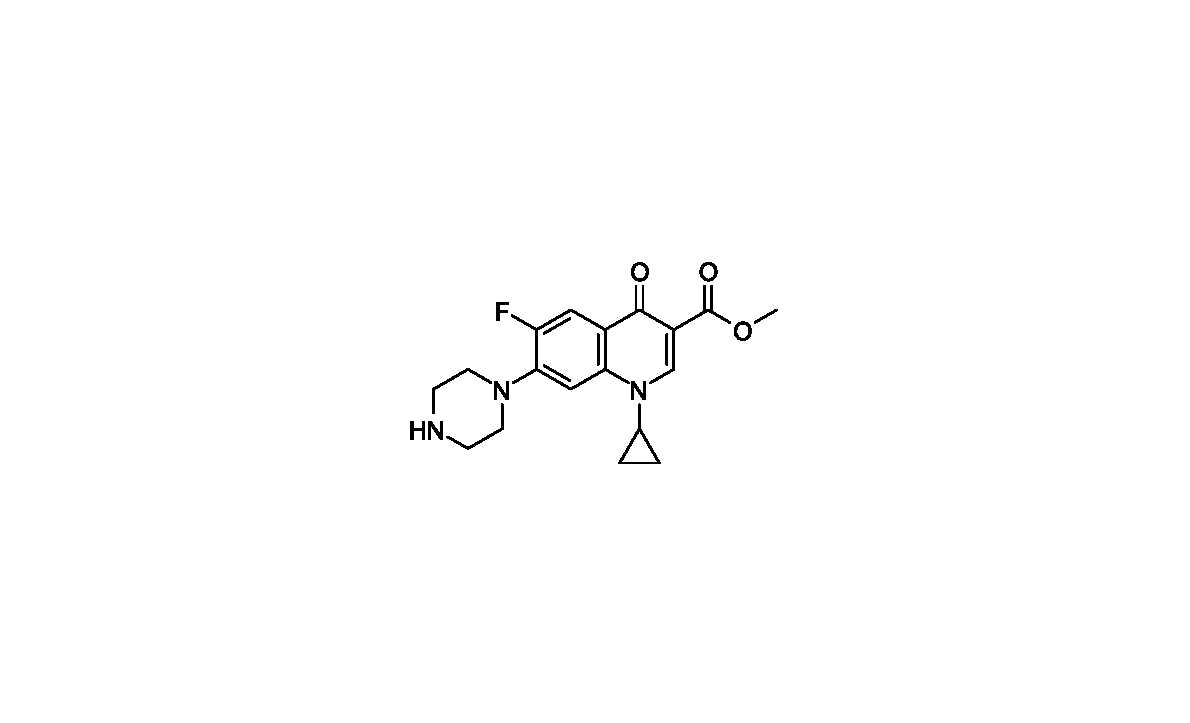
\includegraphics[scale=1]{CipMe.eps}
	\end{center}
\end{scheme}

Ciprofloxacin \compound{cmpd:Cip} (10.0 g, 30 mmol, 1 eq.) and \textit{p}-toluenesulfonic acid (8.60 mg, 44.5 mmol, 1.5 eq.) were refluxed in methanol (500 ml) for 72 h. The mixture was cooled to room temperature and \ce{NaHCO3} (sat., aq., 100 ml) and water (300 ml) were added. The product was extracted with \ce{CH2Cl2} (2$\times$400 ml). The combined organic fractions were dried over \ce{MgSO4} and evaporated under reduced pressure. \compound{cmpd:CipMe} was obtained as a white amorphous solid (9.16 g, 26.5 mmol, 83.3 \%).
\\[1\baselineskip]
\noindent{\textbf{TLC} \textit{R$_f$} = 0.13 (5 \% MeOH/\ce{CH2Cl2})}
\\[1\baselineskip]
%\noindent{\textbf{mp} \textit{T} / $^{\circ}$C = ?? (??)}
%\\[1\baselineskip]
\noindent{\textbf{IR} (neat) $\nu_{max}$ / cm$^{-1}$ = 
	2947.9 (C-H),
	2834.9 (C-H),
	1720.9 (ester C=O),
	1616.8 (quinolone C=O)}
\\[1\baselineskip]
\noindent{\textbf{$^{1}$H NMR} (400 MHz, MeOD) $\delta$ / ppm =
	8.55 (s, 1 H, \textit{ortho} to C(=O)OCH$_3$), 
	7.71 (d, \textit{J} = 13.5 Hz, 1 H, \textit{ortho} to F), 
	7.41 (d, \textit{J} = 7.2 Hz, 1 H, \textit{meta} to F), 
	3.83 (s, 3 H, C\underline{H}$_3$), 
	3.62 (tt, \textit{J} = 7.4, 3.5 Hz, 1 H, NC\underline{H}(CH$_2$)$_2$), 
	3.24 - 3.29 (m, 4 H, HN(CH$_2$C\underline{H}$_2$)CH$_2$C\underline{H}$_2$), 
	3.02 - 3.10 (m, 4 H, HN(C\underline{H}$_2$)C\underline{H}$_2$), 
	1.31 - 1.38 (m, 2 H, NCH(C\underline{H}H)$_2$), 
	1.12 - 1.20 (m, 2 H, NCH(CH\underline{H})$_2$)}
\\[1\baselineskip]
\noindent{\textbf{$^{13}$C NMR} (101 MHz, MeOD) $\delta$ / ppm =
	175.2 (\underline{C}(=O)CC(=O)OCH$_3$), 
	166.8 (\underline{C}(=O)OCH$_3$), 
	154.9 (d, \textit{J} = 248.0 Hz, \textit{ipso} to F), 
	150.1 (\underline{C}=CC(=O)OCH$_3$), 
	146.6 (d, \textit{J} = 10.4 Hz, \textit{ipso} to piperazine), 
	139.9 (\textit{para} to F), 
	123.3 (d, \textit{J} = 6.9 Hz, \textit{para} to piperazine), 
	113.0 (d, \textit{J} = 23.4 Hz, \textit{ortho} to C=O and \textit{ortho} to F), 
	110.1 (\underline{C}C(=O)OCH$_3$), 
	107.1 (d, \textit{J} = 3.5 Hz, \textit{meta} to C=O and \textit{meta} to F), 
	52.3 (\underline{C}H$_3$), 
	51.7 (HN(CH$_2$\underline{C}H$_2$)CH$_2$CH$_2$),
	51.6 (HN(CH$_2$CH$_2$)CH$_2$\underline{C}H$_2$), 
	46.5 (HN(\underline{C}H$_2$)\underline{C}H$_2$), 
	36.4 (N\underline{C}H(CH$_2$)$_2$), 
	8.7 (NCH(\underline{C}H$_2$)$_2$)}
\\[1\baselineskip]
\noindent{\textbf{$^{19}$F NMR} (376.45 MHz, MeOD) $\delta$ / ppm = 
	-124.8 (s, ciprofloxacin F)}
\\[1\baselineskip]
\noindent{\textbf{HRMS} (ESI$^+$) \textit{m}/\textit{z} / Da = 346.1569, [M+H]$^+$ found, [\ce{C18H21FN3O3}]$^+$ requires 346.1567}
\\[1\baselineskip]
The data are consistent with the literature\cite{Sachin2010}.

\subsection{4\hyp{}Bromo\hyp{}\textit{N}\hyp{}(2\hyp{}oxotetrahydrothiophen\hyp{}3\hyp{}yl)butanamide \compound{cmpd:SHL4Br}}

%%LMO\hyp{}2\hyp{}013 (done, pureish), LMO\hyp{}2\hyp{}014 (big, done)

\begin{scheme}[H]
	\begin{center}
		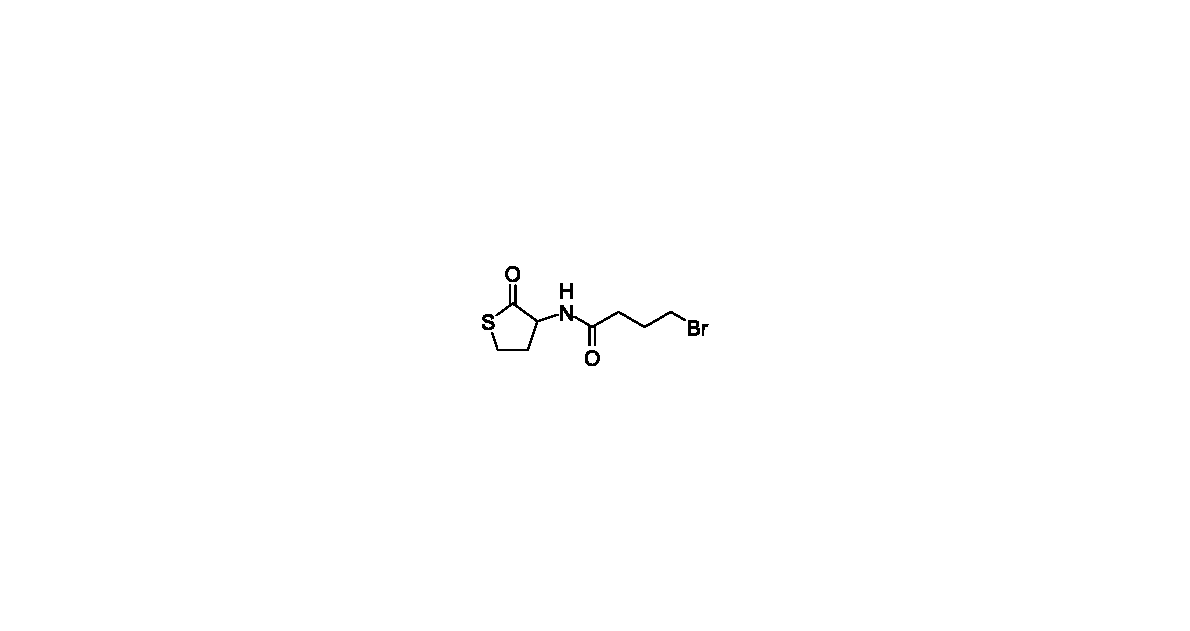
\includegraphics[scale=1]{SHL4Br.eps}
	\end{center}
\end{scheme}

3-Aminodihydrothiophen-2(3\textit{H})-one hydrochloride \compound{cmpd:SHLHCl} (15.0 g, 97.6 mmol, 1 eq.) and \ce{NaHCO3} (16.4 g, 195 mmol, 2 eq.) were added to \ce{CH2Cl2} (150 ml) and water (150 ml). 4-Bromobutyryl chloride \compound{cmpd:Cl4Br} (11.3 ml, 107 mmol, 1.1 eq.) was added dropwise over 45 min at 0 $^{\circ}$C and the mixture was stirred for a further 1 h. The organic layer was separated and the aqueous layer was extracted with a second portion of \ce{CH2Cl2} (150 ml). The combined organic layers were dried over \ce{MgSO4} and evaporated under reduced pressure. \compound{cmpd:SHL4Br} was obtained as a white, amorphous solid (22.7 g, 85.8 mmol, 87.9 \%).
\\[1\baselineskip]
\noindent{\textbf{TLC} \textit{R$_f$} = 0.19 (50 \% EtOAc/PE)}
\\[1\baselineskip]
%\noindent{\textbf{mp} \textit{T} / $^{\circ}$C = ?? (??)}
%\\[1\baselineskip]
\noindent{\textbf{IR} (neat) $\nu_{max}$ / cm$^{-1}$ = 
	3265.9 (amide N-H),
	3063.2 (amide N-H),
	1694.3 (thiolactone C=O),
	1650.5 (amide C=O)}
\\[1\baselineskip]
%\todo{Orientations are not unambiguous without noesy.}
\noindent{\textbf{$^{1}$H NMR} (400 MHz, \ce{CDCl3}) $\delta$ / ppm = 
	6.08 (d, \textit{J} = 6.1 Hz, 1 H, N\underline{H}), 
	4.54 (dt, \textit{J} = 12.9, 6.5 Hz, 1 H, C\underline{H}NH), 
	3.49 (t, \textit{J} = 6.4 Hz, 2 H, C\underline{H}$_2$Br), 
	3.37 (ddd, \textit{J} = 12.2, 11.5, 5.3 Hz, 1 H, SC\underline{H}H), 
	3.26 (ddd, \textit{J} = 11.5, 6.9, 1.3 Hz, 1 H, SCH\underline{H}), 
	2.91 (dddd, \textit{J} = 12.5, 6.7, 5.3, 1.3 Hz, 1 H, SCH$_2$C\underline{H}H), 
	2.45 (t, \textit{J} = 7.4 Hz, 1 H, C(=O)C\underline{H}H), 
	2.45 (t, \textit{J} = 6.8 Hz, 1 H, C(=O)CH\underline{H}), 
	2.20 (quin, \textit{J} = 6.7 Hz, 1 H, C(=O)CH$_2$C\underline{H}$_2$), 
	1.96 (dddd, \textit{J} = 12.7, 12.5, 12.2, 7.0 Hz, 1 H, SCH$_2$CH\underline{H})}
\\[1\baselineskip]
\noindent{\textbf{$^{13}$C NMR} (101 MHz, \ce{CDCl3}) $\delta$ / ppm = 
	205.4 (S\underline{C}(=O)), 
	172.1 (NH\underline{C}(=O)), 
	59.4 (\underline{C}HNH), 
	34.1 (C(=O)\underline{C}H$_2$), 
	33.1 (\underline{C}H$_2$Br), 
	31.8 (SCH$_2$\underline{C}H$_2$), 
	28.0 (C(=O)CH$_2$\underline{C}H$_2$), 
	27.5 (S\underline{C}H$_2$)}
\\[1\baselineskip]
\noindent{\textbf{HRMS} (ESI$^+$) The compound does not ionise.}
\\[1\baselineskip]
The compound has been synthesised previously\cite{Ganguly2011,Iyer2012} but characterisation was not published.



\subsection{Methyl 1\hyp{}cyclopropyl\hyp{}6\hyp{}fluoro\hyp{}4\hyp{}oxo\hyp{}7\hyp{}(4\hyp{}(4\hyp{}oxo\hyp{}4\hyp{}((2\hyp{}oxotetrahydrothiophen\hyp{}3\hyp{}yl)amino)butyl)pip\allowbreak erazin\hyp{}1\hyp{}yl)\hyp{}1,4\hyp{}dihydroquinoline\hyp{}3\hyp{}carboxylate \compound{cmpd:SHL4CipMe}}

%%LMO\hyp{}2\hyp{}017 (done, poor yield), LMO\hyp{}2\hyp{}021 (big, done, poor yield)

\begin{scheme}[H]
	\begin{center}
		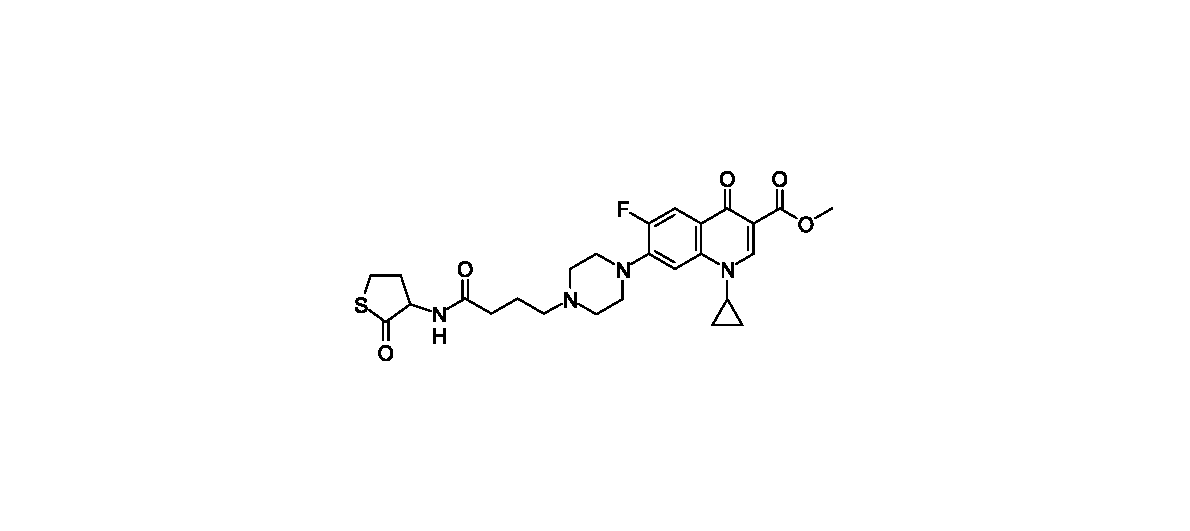
\includegraphics[scale=1]{SHL4CipMe.eps}
	\end{center}
\end{scheme}

Methyl 1\hyp{}cyclopropyl\hyp{}6\hyp{}fluoro\hyp{}4\hyp{}oxo\hyp{}7\hyp{}(piperazin\hyp{}1\hyp{}yl)\hyp{}1,4\hyp{}dihydroquinoline\hyp{}3\hyp{}carboxylate \compound{cmpd:CipMe} (50 mg, 0.145 mmol, 1 eq.),
4\hyp{}bromo\hyp{}\textit{N}\hyp{}(2\hyp{}oxotetrahydrothiophen\hyp{}3\hyp{}yl)butanamide \compound{cmpd:SHL4Br} (34.5 mg, 0.145 mmol, 1 eq.)
and \ce{K2CO3} (20 mg, 0.145 mmol, 1 eq.) were stirred in acetonitrile (2 ml) at 50 $^{\circ}$C under argon. After 24 h a further portion of \compound{cmpd:SHL4Br} (34.5 mg, 0.145 mmol, 1 eq.) was added. After another 24 h a further portion was added (69.0 mg, 0.290 mmol, 2 eq.). After another 24 h the temperature was raised so the mixture was at reflux. After a final 24 h the precipitate was filtered off and the filtrate was purified by column chromatography (\ce{SiO2}, 5-10 \% MeOH/\ce{CH2Cl2}) followed by preparatory HPLC (5-95 \% acetonitrile/water over 20 min). \compound{cmpd:SHL4CipMe} was obtained as a cream-coloured amorphous solid (9.4 mg, 0.018 mmol, 12.2 \%).
\\[1\baselineskip]
\noindent{\textbf{TLC} \textit{R$_f$} = 0.47 (10 \% MeOH/\ce{CH2Cl2})}
\\[1\baselineskip]
%\noindent{\textbf{mp} \textit{T} / $^{\circ}$C = ?? (??)}
%\\[1\baselineskip]
\noindent{\textbf{IR} (neat) $\nu_{max}$ / cm$^{-1}$ = 
	2944.2 (C-H),
	2832.4 (C-H),
	1722.4 (ester C=O),
	1700.4 (thiolactone C=O),
	1669.6 (amide C=O),
	1617.3 (quinolone C=O)}
\\[1\baselineskip]
\noindent{\textbf{$^{1}$H NMR} (500 MHz, MeOD) $\delta$ / ppm = 
	8.53 (s, 1 H, \textit{ortho} to C(=O)OCH$_3$), 
	7.68 (d, J=13.4 Hz, 1 H, \textit{ortho} to F), 
	7.41 (d, J=7.3 Hz, 1 H, \textit{meta} to F), 
	4.67 (dd, J=12.9, 6.9 Hz, 1 H, C\underline{H}NH), 
	3.83 (s, 3 H, OC\underline{H}$_3$), 
	3.61 (tt, J=6.9, 4.1 Hz, 1 H, NC\underline{H}(CH$_2$)$_2$), 
	3.39 - 3.49 (m, 5 H, SC\underline{H}H), 
	3.26 - 3.33 (m, 1 H, SCH\underline{H} and CH$_2$CH$_2$CH$_2$N(CH$_2$C\underline{H}$_2$)CH$_2$C\underline{H}$_2$), 
	2.93 - 3.03 (m, 4 H, CH$_2$CH$_2$CH$_2$N(C\underline{H}$_2$)C\underline{H}$_2$), 
	2.79 (br. t, J=7.2, 7.2 Hz, 2 H, C(=O)CH$_2$CH$_2$C\underline{H}$_2$), 
	2.59 (dddd, J=12.4, 6.9, 5.4, 1.4 Hz, 1 H, SCH$_2$C\underline{H}H), 
	2.39 (t, J=7.20 Hz, 1 H, C(=O)C\underline{H}H), 
	2.38 (t, J=6.94 Hz, 1 H, C(=O)CH\underline{H}), 
	2.18 (qd, J=12.4, 7.0 Hz, 1 H, SCH$_2$CH\underline{H}), 
	1.97 (quin, J=7.2 Hz, 2 H, C(=O)CH$_2$C\underline{H}$_2$), 
	1.32 - 1.37 (m, 2 H, NCH(C\underline{H}H)$_2$), 
	1.13 - 1.19 (m, 2 H, NCH(CH\underline{H})$_2$)}
\\[1\baselineskip]
\noindent{\textbf{$^{13}$C NMR} (126 MHz, MeOD) $\delta$ / ppm = 
	207.0 (S\underline{C}(=O)), 
	175.7 (NH\underline{C}(=O)), 
	175.1 (\underline{C}(=O)CC(=O)OCH$_3$), 
	166.6 (\underline{C}(=O)OCH$_3$), 
	154.7 (d, J=249.0 Hz, \textit{ipso} to F), 
	150.2 (s, \underline{C}H=CC(=O)OCH$_3$), 
	145.6 (d, J=10.6 Hz, \textit{ipso} to piperazine), 
	139.8 (\textit{para} to F), 
	123.5 (d, J=6.9 Hz, \textit{para} to piperazine), 
	113.1 (d, J=23.6 Hz, \textit{ortho} to C=O and \textit{ortho} to F), 
	110.0 (\underline{C}C(=O)OCH$_3$), 
	107.4 (\textit{meta} to C=O and \textit{meta} to F), 
	60.2 (\underline{C}HNH), 
	58.5 (C(=O)CH$_2$CH$_2$\underline{C}H$_2$), 
	53.8 (CH$_2$CH$_2$CH$_2$N(\underline{C}H$_2$)\underline{C}H$_2$), 
	52.3 (O\underline{C}H$_3$), 
	50.1 (CH$_2$CH$_2$CH$_2$N(CH$_2$\underline{C}H$_2$)CH$_2$CH$_2$), 
	50.0 (CH$_2$CH$_2$CH$_2$N(CH$_2$CH$_2$)CH$_2$\underline{C}H$_2$), 
	36.5 (N\underline{C}H(CH$_2$)$_2$), 
	34.5 (C(=O)\underline{C}H$_2$), 
	31.7 (SCH$_2$\underline{C}H$_2$), 
	28.1 (S\underline{C}H$_2$), 
	22.9 (C(=O)CH$_2$\underline{C}H$_2$CH$_2$), 
	8.7 (NCH(\underline{C}H$_2$)$_2$)}
\\[1\baselineskip]
\noindent{\textbf{$^{19}$F NMR} (376.45 MHz, MeOD) $\delta$ / ppm = 
	-125.4 (s, ciprofloxacin F)}
\\[1\baselineskip]
\noindent{\textbf{HRMS} (ESI$^+$) \textit{m}/\textit{z} / Da = 531.2083, [M+H]$^+$ found, [\ce{C26H32FN4O5S}]$^+$ requires 531.2077}
%High-resolution
%mass spectrometry C26
%H32 O5 N4 F1
%32\textit{S}1 531.20667
%(error +- 0.992 ppm).
\\[1\baselineskip]
The compound has been synthesised previously\cite{Ganguly2011,Iyer2012}. Only HRMS characterisation was published, and this agrees with the result above.
%
%\subsection{1\hyp{}cyclopropyl\hyp{}6\hyp{}fluoro\hyp{}4\hyp{}oxo\hyp{}7\hyp{}(4\hyp{}(4\hyp{}oxo\hyp{}4\hyp{}((2\hyp{}oxotetrahydrothiophen\hyp{}3\hyp{}yl)am\hyp{}ino)butyl)piperazin\hyp{}1\hyp{}yl)\hyp{}1,4\hyp{}dihydroquinoline\hyp{}3\hyp{}carboxylic acid \compound{cmpd:SHL4Cip}}
%
%%%LMO\hyp{}2\hyp{}025 (hydrolyses lactone), LMO\hyp{}2\hyp{}026 (??)
%
%\begin{scheme}[H]
%	\begin{center}
%		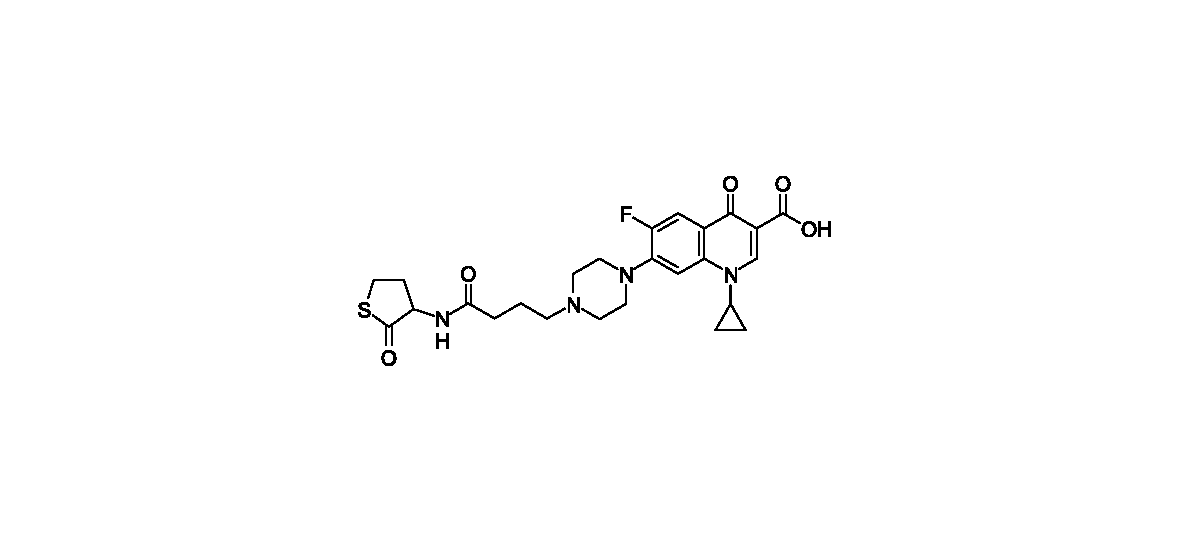
\includegraphics[scale=1]{SHL4Cip.eps}
%	\end{center}
%\end{scheme}

\subsection{4\hyp{}Azido\hyp{}\textit{N}\hyp{}(2\hyp{}oxotetrahydrothiophen\hyp{}3\hyp{}yl)butanamide \compound{cmpd:SHL4N3}}

%%LMO\hyp{}2\hyp{}018 (done, DMF), LMO\hyp{}2\hyp{}019 (done, MeCN), LMO\hyp{}2\hyp{} (done, big, MeCN)

\begin{scheme}[H]
	\begin{center}
		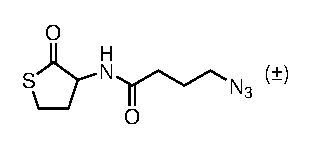
\includegraphics[scale=1]{SHL4N3.eps}
	\end{center}
\end{scheme}

4\hyp{}Bromo\hyp{}\textit{N}\hyp{}(2\hyp{}oxotetrahydrothiophen\hyp{}3\hyp{}yl)butanamide \compound{cmpd:SHL4Br} (6.00 g, 27.0 mmol, 1 eq.) and \ce{NaN3} (3.51 g, 54.1 mmol, 2 eq.) were refluxed in acetonitrile (120 ml) for 1.5 h. The solvent was evaporated under reduced pressure and the residue was partitioned between water (150 ml) and \ce{CH2Cl2} (150 ml). The aqueous layer was extracted twice more with \ce{CH2Cl2} (2$\times$150 ml) and the combined organic fractions were dried with \ce{MgSO4} and evaporated under reduced pressure. \compound{cmpd:SHL4N3} was obtained as a yellow, sticky solid (4.60 g, 20.1 mmol, 89.3 \%).
\\[1\baselineskip]
\noindent{\textbf{TLC} \textit{R$_f$} = 0.19 (50 \% EtOAc/PE)}
\\[1\baselineskip]
%\noindent{\textbf{mp} \textit{T} / $^{\circ}$C = ?? (??)}
%\\[1\baselineskip]
\noindent{\textbf{IR} (neat) $\nu_{max}$ / cm$^{-1}$ = 
	3285.6 (N-H),
	2963.9 (C-H),
	2100.2 (azide),
	1697.4 (thiolactone C=O),
	1647.4 (amide C=O)}
\\[1\baselineskip]
\noindent{\textbf{$^{1}$H NMR} (400 MHz, \ce{CDCl3}) $\delta$ / ppm = 
	6.71 (d, \textit{J} = 7.3 Hz, 1 H, N\underline{H}), 
	4.54 (dt, \textit{J} = 13.0, 7.0 Hz, 1 H, C\underline{H}NH), 
	3.30 (t, \textit{J} = 6.7 Hz, 2 H, C\underline{H}$_2$N$_3$), 
	3.31 (td, \textit{J} = 11.7, 5.3 Hz, 1 H, 1 H, SC\underline{H}H), 
	3.19 (ddd, \textit{J} = 11.3, 7.0, 1.2 Hz, 1 H, SCH\underline{H}), 
	2.70 (dddd, \textit{J} = 12.4, 6.8, 5.3, 1.2 Hz, 1 H, SCH$_2$C\underline{H}H), 
	2.29 (t, \textit{J} = 7.5 Hz, 1 H, C(=O)C\underline{H}H), 
	2.28 (t, \textit{J} = 7.1 Hz, 1 H, C(=O)CH\underline{H}), 
	1.97 (qd, \textit{J} = 12.4, 7.0 Hz, 1 H, SCH$_2$CH\underline{H}), 
	1.85 (quin, \textit{J} = 6.9 Hz, 2 H, C(=O)CH$_2$C\underline{H}$_2$)}
\\[1\baselineskip]
\noindent{\textbf{$^{13}$C NMR} (101 MHz, \ce{CDCl3}) $\delta$ / ppm = 
	205.4 (S\underline{C}(=O)), 
	172.3 (NH\underline{C}(=O)), 
	59.4 (\underline{C}HNH), 
	50.6 (\underline{C}H$_2$N$_3$), 
	32.8 (C(=O)\underline{C}H$_2$), 
	31.8 (SCH$_2$\underline{C}H$_2$), 
	27.5 (S\underline{C}H$_2$), 
	24.6 (C(=O)CH$_2$\underline{C}H$_2$)}
\\[1\baselineskip]
\noindent{\textbf{HRMS} (ESI$^+$) \textit{m}/\textit{z} / Da = 251.0565, [M+Na]$^+$ found, [\ce{C8H12N4NaO2S}]$^+$ requires 251.0573}
\\[1\baselineskip]
The compound has not been reported previously.

\subsection{1\hyp{}Cyclopropyl\hyp{}6\hyp{}fluoro\hyp{}4\hyp{}oxo\hyp{}7\hyp{}(4\hyp{}(4\hyp{}(1\hyp{}(4\hyp{}oxo\hyp{}4\hyp{}((2\hyp{}oxotetrahydrothiophen\hyp{}3\hyp{}yl)amino)butyl)\hyp{}1\textit{H}\hyp{}1,2,3\hyp{}triazol\hyp{}4\hyp{}yl)butyl)piperazin\hyp{}1\hyp{}yl)\hyp{}1,4\hyp{}dihydroquin\allowbreak o\allowbreak l\allowbreak ine\hyp{}3\hyp{}carboxylic acid \compound{cmpd:SHL4T4Cip}}

%%LMO\hyp{}2\hyp{}022 (CuI, stalled but then went?)

\begin{scheme}[H]
	\begin{center}
		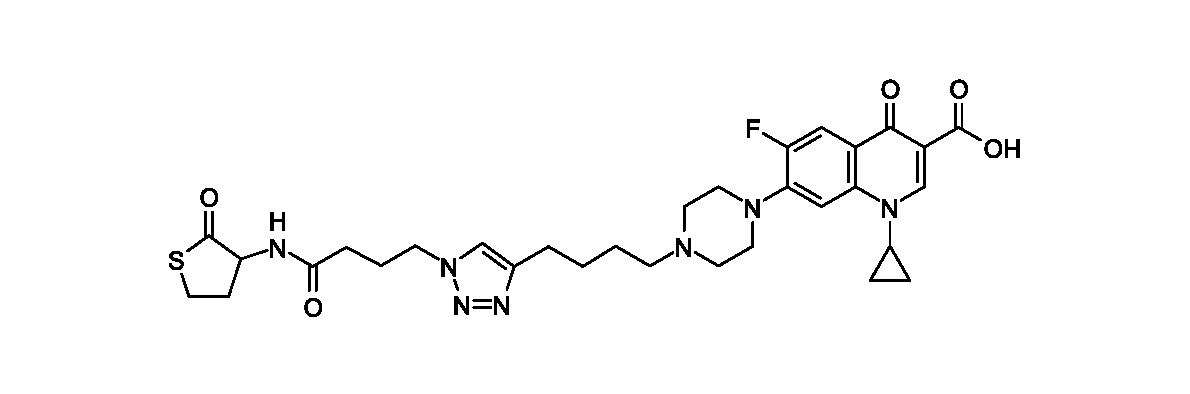
\includegraphics[scale=1]{SHL4T4Cip.eps}
	\end{center}
\end{scheme}

1-Cyclopropyl-6-fluoro-7-(4-(hex-5-yn-1-yl)piperazin-1-yl)-4-oxo-1,4\hyp{}dihydro\-quinoline-3-carboxylic acid \compound{cmpd:Y4Cip} (15 mg, 36.7 $\mu$mol, 1 eq.) and 
4\hyp{}azido\hyp{}\textit{N}\hyp{}(2\hyp{}oxotetrahydrothiophen\hyp{}3\hyp{}yl)butanamide \compound{cmpd:SHL4N3} (12.5 mg, 55.1 $\mu$mol, 1.5 eq.) 
were dissolved in 1:9:10 water/\textit{t}-BuOH/DMSO (3 ml), and the mixture was degassed by bubbling \ce{N2} through it. 
A solution of \ce{CuSO4} and THPTA (182 $\mu$l, 18.2 $\mu$mol, 0.5 eq. 100 mM, aq.) was added, followed by a solution of sodium ascorbate (367 $\mu$l, 36.7 $\mu$mol, 1 eq., 100 mM, aq.). 
The mixture was stirred at r.t. under argon for 4 d. Water (10 ml) and 10 \% \textit{i}-PrOH/\ce{CHCl3} (10 ml) were added, the organic layer was separated and the aqueous layer was extracted again with 10 \% \textit{i}-PrOH/\ce{CHCl3} (2$\times$10 ml). The combined organic layers were dried with \ce{MgSO4} and evaporated under reduced pressure. The residue was purified by preparatory HPLC (5-95 \% acetonitrile/water over 20 min). 
The combined pure fractions were evaporated under reduced pressure and then partitioned between \ce{NaHCO3} (aq., sat., 50 ml) and 10 \% \textit{i}-PrOH/\ce{CHCl3} (50 ml). The organic layer was dried with \ce{MgSO4} and evaporated under reduced pressure.
\compound{cmpd:SHL4T4Cip} was obtained as a white amorphous solid (16.5 mg, 25.9 $\mu$mol, 70.6 \%).
\\[1\baselineskip]
%\noindent{\textbf{TLC} \textit{R$_f$} = ?? (??)}
%\\[1\baselineskip]
%\noindent{\textbf{mp} \textit{T} / $^{\circ}$C = ?? (??)}
%\\[1\baselineskip]
\noindent{\textbf{IR} (neat) $\nu_{max}$ / cm$^{-1}$ = 
	2918.8 (C-H),
	1712.7 (carboxylic acid C=O and thiolactone C=O),
	1657.6 (amide C=O),
	1626.8 (quinolone C=O),
	1616.2 (triazole)}
\\[1\baselineskip]
\noindent{\textbf{$^{1}$H NMR} (500 MHz, DMSO d$_6$) $\delta$ / ppm = 
	15.23 (br s, 1 H, C(=O)O\underline{H}), 
	8.66 (s, 1 H, \textit{ortho} to C(=O)OH), 
	8.23 (d, J=8.5 Hz, 1 H, N\underline{H}), 
	7.90 (d, J=13.4 Hz, 1 H, \textit{ortho} to F), 
	7.84 (s, 1 H, C\underline{H}=CCH$_2$), 
	7.56 (d, J=7.5 Hz, 1 H, \textit{meta} to F), 
	4.59 (ddd, J=12.7, 8.4, 6.8 Hz, 1 H, C\underline{H}NH), 
	4.31 (t, J=7.0 Hz, 2 H, C\underline{H}$_2$NCH=C), 
	3.80 - 3.86 (6.9, 4.0 Hz, 1 H, NC\underline{H}(CH$_2$)$_2$), 
	3.34 - 3.37 (m, 1 H, SC\underline{H}H), 
	3.32 (br t, J=4.1 Hz, 4 H, CH$_2$CH$_2$CH$_2$N(CH$_2$C\underline{H}$_2$)CH$_2$C\underline{H}$_2$), 
	3.27 (ddd, J=11.1, 6.9, 1.4 Hz, 1 H, SCH\underline{H}), 
	2.64 (t, J=7.6 Hz, 2 H, CH=CC\underline{H}$_2$), 
	2.57 (br t, J=4.7 Hz, 4 H, CH$_2$CH$_2$CH$_2$N(C\underline{H}$_2$)C\underline{H}$_2$), 
	2.34 - 2.44 (m, 3 H, SCH$_2$C\underline{H}H and CH=CCH$_2$CH$_2$CH$_2$C\underline{H}$_2$), 
	2.12 (t, J=7.9 Hz, 1 H, C(=O)C\underline{H}H), 
	2.12 (t, J=7.0 Hz, 1 H, C(=O)CH\underline{H}), 
	2.04 (m, 3 H, SCH$_2$CH\underline{H} and C(=O)CH$_2$C\underline{H}$_2$), 
	1.64 (quin, J=7.5 Hz, 2 H, CH=CCH$_2$C\underline{H}$_2$), 
	1.51 (quin, J=7.5 Hz, 2 H, CH=CCH$_2$CH$_2$C\underline{H}$_2$), 
	1.28 - 1.34 (m, 2 H, NCH(C\underline{H}H)$_2$), 
	1.15 - 1.20 (m, 2 H, NCH(CH\underline{H})$_2$)}
\\[1\baselineskip]
\noindent{\textbf{$^{13}$C NMR} (126 MHz, DMSO d$_6$) $\delta$ / ppm = 
	205.6 (S\underline{C}(=O)), 
	176.4 (\underline{C}(=O)CC(=O)OH), 
	171.4 (NH\underline{C}(=O)), 
	166.0 (\underline{C}(=O)OH), 
	153.1 (d, J=249.3 Hz, \textit{ortho} to F), 
	148.0 (\underline{C}H=CC(=O)OH), 
	146.9 (CH=\underline{C}CH$_2$), 
	145.3 (d, J=10.1 Hz, \textit{ipso} to piperazine), 
	139.2 (\textit{para} to F), 
	121.8 (\underline{C}H=CCH$_2$), 
	118.6 (d, J=7.7 Hz, \textit{para} to piperazine), 
	111.0 (d, J=23.3 Hz, \textit{ortho} to C=O and \textit{ortho} to F), 
	106.7 (\underline{C}C(=O)OH), 
	106.4 (d, J=2.9 Hz, \textit{meta} to C=O and \textit{meta} to F), 
	58.2 (SC(=O)\underline{C}HNH), 
	57.4 (CH=CCH$_2$CH$_2$CH$_2$\underline{C}H$_2$N), 
	52.4 (CH$_2$CH$_2$CH$_2$N(\underline{C}H$_2$)\underline{C}H$_2$), 
	49.5 (CH$_2$CH$_2$CH$_2$N(CH$_2$\underline{C}H$_2$)CH$_2$CH$_2$), 
	49.5 (CH$_2$CH$_2$CH$_2$N(CH$_2$CH$_2$)CH$_2$\underline{C}H$_2$), 
	48.6 (\underline{C}H$_2$NCH=C), 
	35.9 (N\underline{C}H(CH$_2$)$_2$), 
	31.9 (NHC(=O)\underline{C}H$_2$), 
	30.1 (\underline{C}H$_2$CHNH), 
	26.9 (CH=CCH$_2$\underline{C}H$_2$), 
	26.8 (S\underline{C}H$_2$), 
	25.9 (NHC(=O)\allowbreak CH$_2$\underline{C}H$_2$), 
	25.8 (CH=CCH$_2$CH$_2$\underline{C}H$_2$), 
	25.0 (CH=C\underline{C}H$_2$), 
	7.6 (NCH(\underline{C}H$_2$)$_2$)}
\\[1\baselineskip]
\noindent{\textbf{$^{19}$F NMR} (376.45 MHz, MeOD) $\delta$ / ppm = 
	-124.9 (s, ciprofloxacin F)}
\\[1\baselineskip]
\noindent{\textbf{HRMS} (ESI$^+$) \textit{m}/\textit{z} / Da = 640.2739, [M+H]$^+$ found, [\ce{C31H39FN7O5S}]$^+$ requires 640. 2712}


\subsection{1\hyp{}Cyclopropyl\hyp{}6\hyp{}fluoro\hyp{}4\hyp{}oxo\hyp{}7\hyp{}(4\hyp{}((((4\hyp{}(1\hyp{}(4\hyp{}oxo\hyp{}4\hyp{}((2\hyp{}oxotetrahydrothioph\hfill\allowbreak en\hyp{}3\hyp{}yl)amino)butyl)\hyp{}1\textit{H}\hyp{}1,2,3\hyp{}triazol\hyp{}4\hyp{}yl)butanoyl)oxy)methoxy)carbonyl)\hfill\allowbreak pip\allowbreak e\allowbreak razin\hyp{}1\hyp{}yl)\hyp{}1,4\hyp{}dihydroquinoline\hyp{}3\hyp{}carboxylic acid \compound{cmpd:SHL4THCip}}


%%LMO\hyp{}2\hyp{}023 (partially done?? - DONE. Think was wrongly labelled as the methyl version for NMR)

\begin{scheme}[H]
	\begin{center}
		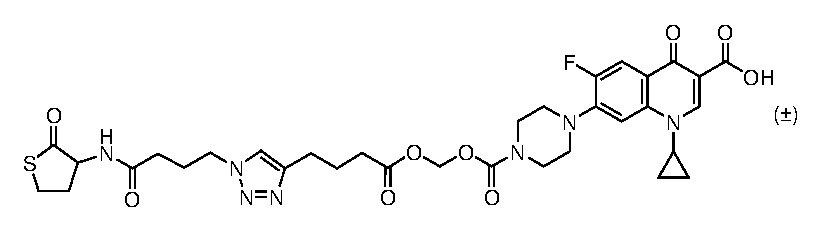
\includegraphics[scale=1]{SHL4THCip.eps}
	\end{center}
\end{scheme}

1-Cyclopropyl-6-fluoro-7-(4-(((hex-5-ynoyloxy)methoxy)carbonyl)piperazin-1-yl)-4-oxo-1,4-dihydroquinoline\hyp{}3-\hfill\allowbreak carboxylic acid \compound{cmpd:Y4OHOCip} (203 mg, 0.407 mmol, 1 eq.), 4\hyp{}azido\hyp{}\textit{N}\hyp{}(2\hyp{}oxotetrahydrothiophen\hyp{}3\hyp{}yl)butanamide \compound{cmpd:SHL4N3} (92.8 mg, 0.407 mmol, 1 eq.), CuI (40 mg, 0.190 mmol, 0.5 eq.) and DIPEA (0.356 ml, 0.264 mg, 2.04 mmol, 5 eq.) were stirred in \ce{CH2Cl2} (18.6 ml) at r.t. under Ar for 3 h. The mixture was fitered and the filtrate was dry-loaded onto \ce{SiO2} and purified by column chromatography (\ce{SiO2}, 5-10 \% MeOH/\ce{CH2Cl2}). \compound{cmpd:SHL4THCip} was obtained as pale brown/yellow amorphous solid (14.7 mg, 20.2 $\mu$mol, 5.0 \%).
\\[1\baselineskip]
\noindent{\textbf{TLC} \textit{R$_f$} = 0.40 (5 \% \ce{CH2Cl2}/MeOH)}
\\[1\baselineskip]
%\noindent{\textbf{mp} \textit{T} / $^{\circ}$C = ?? (??)}
%\\[1\baselineskip]
\noindent{\textbf{IR} (neat) $\nu_{max}$ / cm$^{-1}$ = 
	3054.9 (C-H),
	1715.8 (carboxylic acid C=O and ester C=O),
	1696.2 (carbamate C=O and thiolactone C=O),
	1651.2 (amide C=O),
	1629.2 (quinolone C=O)}
	%no triazole
\\[1\baselineskip]
\noindent{\textbf{$^{1}$H NMR} (400 MHz, DMSO d$_6$) $\delta$ / ppm = 
	15.16 (br s, 1 H, C(=O)O\underline{H}), 
	8.65 (s, 1 H, \textit{ortho} to C(=O)OH), 
	8.21 (d, \textit{J} = 8.5 Hz, 1 H, N\underline{H}), 
	7.89 (d, \textit{J} = 13.1 Hz, 1 H, \textit{ortho} to F), 
	7.85 (s, 1 H, C\underline{H}=CCH$_2$), 
	7.57 (d, \textit{J} = 7.4 Hz, 1 H, \textit{meta} to F), 
	5.74 (s, 1 H, OC\underline{H}$_2$O), 
	4.58 (ddd, \textit{J} = 12.6, 8.1, 7.2 Hz, 1 H, C\underline{H}NH), 
	4.30 (t, \textit{J} = 6.9 Hz, 2 H, C(=O)CH$_2$CH$_2$C\underline{H}$_2$N), 
	3.80 (tt, \textit{J} = 6.9, 3.6 Hz, 1 H, NC\underline{H}(CH$_2$)$_2$), 
	3.62 (br t, \textit{J} = 5.2, 5.2 Hz, 4 H, C(=O)N(C\underline{H}$_2$)C\underline{H}$_2$), 
	3.38 (td, \textit{J} = 11.4, 5.5 Hz, 1 H, SC\underline{H}H), 
	3.34 (br. s, 4 H, C(=O)N(CH$_2$C\underline{H}$_2$)CH$_2$C\underline{H}$_2$), 
	3.27 (ddd, \textit{J} = 11.0, 6.9, 1.6 Hz, 1 H, SCH\underline{H}), 
	2.64 (t, \textit{J} = 7.6 Hz, 2 H, CH=CC\underline{H}$_2$), 
	2.44 (t, \textit{J} = 7.5 Hz, 2 H, C\underline{H}$_2$C(=O)O), 
	2.40 (dddd, \textit{J} = 12.3, 6.8, 5.4, 1.4 Hz, 1 H, SCH$_2$C\underline{H}H), 
	2.12 (t, \textit{J} = 7.8 Hz, 1 H, NHC(=O)C\underline{H}H), 
	2.12 (t, \textit{J} = 6.8 Hz, 1 H, NHC(=O)CH\underline{H}), 
	1.98 - 2.07 (m, 3 H, SCH$_2$C\underline{H}H and NHC(=O)CH$_2$C\underline{H}$_2$), 
	1.86 (quin, \textit{J} = 7.5 Hz, 2 H, CH=CCH$_2$C\underline{H}$_2$), 
	1.29 - 1.36 (m, 2 H, NCH(C\underline{H}H)$_2$), 
	1.14 - 1.21 (m, 2 H, NCH(CH\underline{H})$_2$)}
\\[1\baselineskip]
\noindent{\textbf{$^{13}$C NMR} (101 MHz, DMSO d$_6$) $\delta$ / ppm = 
	205.5 (S\underline{C}(=O)), 
	176.4 (\underline{C}(=O)CC(=O)OH), 
	171.8 (\underline{C}(=O)OCH$_2$O), 
	171.3 (NH\underline{C}(=O)), 
	165.9 (\underline{C}(=O)OH), 
	152.8 (d, \textit{J} = 249.7 Hz, \textit{ipso} to F), 
	152.9 (O\underline{C}(=O)N), 
	148.1 (\underline{C}H=CC(=O)\allowbreak OH), 
	146.0 (CH=\underline{C}CH$_2$), 
	144.9 (d, \textit{J} = 9.6 Hz, \textit{ipso} to piperazine), 
	139.1 (\textit{para} to F), 
	122.0 (\underline{C}H=CCH$_2$), 
	118.9 (d, \textit{J} = 7.5 Hz, \textit{para} to piperazine), 
	111.0 (d, \textit{J} = 23.5 Hz, \textit{ortho} to C=O and \textit{ortho} to F), 
	106.8 (\underline{C}C(=O)OH, and \textit{meta} to C=O and \textit{meta} to F), 
	80.3 (O\underline{C}H$_2$O), 
	58.2 (\underline{C}HNH), 
	49.1 (C(=O)N(CH$_2$\underline{C}H$_2$)CH$_2$CH$_2$), 
	49.1 (C(=O)N(CH$_2$CH$_2$)CH$_2$\underline{C}H$_2$), 
	48.6 (C(=O)CH$_2$CH$_2$\underline{C}H$_2$N), 
	43.4 (N(\underline{C}H$_2$)CH$_2$), 
	43.0 (N(CH$_2$)\underline{C}H$_2$), 
	35.9 (N\underline{C}H\allowbreak (CH$_2$)$_2$), 
	32.7 (CH=CCH$_2$CH$_2$\underline{C}H$_2$C(=O)), 
	31.8 (NH\underline{C}(=O)\underline{C}H$_2$), 
	30.1 (SCH$_2$\underline{C}H$_2$), 
	26.8 (S\underline{C}H$_2$), 
	25.8 (C(=O)\allowbreak CH$_2$\underline{C}H$_2$CH$_2$N), 
	24.2 (CH=C\underline{C}H$_2$CH$_2$CH$_2$C(=O)), 
	24.0 (CH=CCH$_2$\underline{C}H$_2$CH$_2$C(=O)), 
	7.6 (NCH(\underline{C}H$_2$)$_2$)}
\\[1\baselineskip]
%\noindent{\textbf{$^{19}$F NMR} (376.45 MHz, DMSO d$_6$) $\delta$ / ppm = ??}\todo{no F}
%\\[1\baselineskip]
\noindent{\textbf{HRMS} (ESI$^+$) \textit{m}/\textit{z} / Da = 728.2502, [M+H]$^+$ found, [\ce{C33H39FN7O9S}]$^+$ requires 728.2503}
\\[1\baselineskip]
The compound has not been reported previously.

%\subsection{1\hyp{}Cyclopropyl\hyp{}6\hyp{}fluoro\hyp{}4\hyp{}oxo\hyp{}7\hyp{}(4\hyp{}((1\hyp{}((4\hyp{}(1\hyp{}(4\hyp{}oxo\hyp{}4\hyp{}((2\hyp{}oxotetrahydrothioph\hyp{}en\hyp{}3\hyp{}yl)amino)butyl)\hyp{}1H\hyp{}1,2,3\hyp{}triazol\hyp{}4\hyp{}yl)butanoyl)oxy)ethoxy)carbonyl)pip\hyp{}erazin\hyp{}1\hyp{}yl)\hyp{}1,4\hyp{}dihydroquinoline\hyp{}3\hyp{}carboxylic acid \compound{cmpd:SHL4TMeCip}}
%
%%%LMO\hyp{}2\hyp{}024 (partially done?), LMO\hyp{}2\hyp{}027 (too little to tell)
%
%\begin{scheme}[H]
%	\begin{center}
%		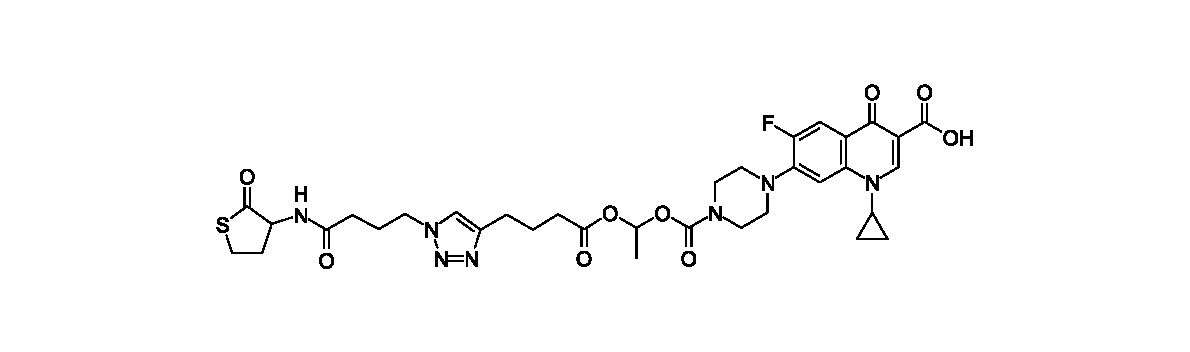
\includegraphics[scale=1]{SHL4TMeCip.eps}
%	\end{center}
%\end{scheme}
%
%Method??
%white amorphous solid
%1.2 mg, 1.6 $\mu$mol
%\\[1\baselineskip]
%\noindent{\textbf{TLC} \textit{R$_f$} = 0.33 (10 \% MeOH/\ce{CH2Cl2})}
%\\[1\baselineskip]
%%\noindent{\textbf{mp} \textit{T} / $^{\circ}$C = ?? (??)}
%%\\[1\baselineskip]
%\noindent{\textbf{IR} (neat) $\nu_{max}$ / cm$^{-1}$ = ??} 
%\\[1\baselineskip]
%\noindent{\textbf{$^{1}$H NMR} (400 MHz, MeOD) $\delta$ / ppm = ??}
%\\[1\baselineskip]
%\noindent{\textbf{$^{13}$C NMR} (101 MHz, MeOD) $\delta$ / ppm = ??}
%\\[1\baselineskip]
%\noindent{\textbf{$^{19}$F NMR} (376.45 MHz, MeOD) $\delta$ / ppm = ??}
%\\[1\baselineskip]
%\noindent{\textbf{HRMS} (ESI$^+$) \textit{m}/\textit{z} / Da = 742.2670, [M+H]$^+$ found, [\ce{C34H41FN7O9S}]$^+$ requires 742.2671}

\subsection{4\hyp{}Bromo\hyp{}\textit{N}\hyp{}(2\hyp{}methoxyphenyl)butanamide \compound{cmpd:2MeOA4Br}}

%%LMO\hyp{}2\hyp{}028 (done)

\begin{scheme}[H]
	\begin{center}
		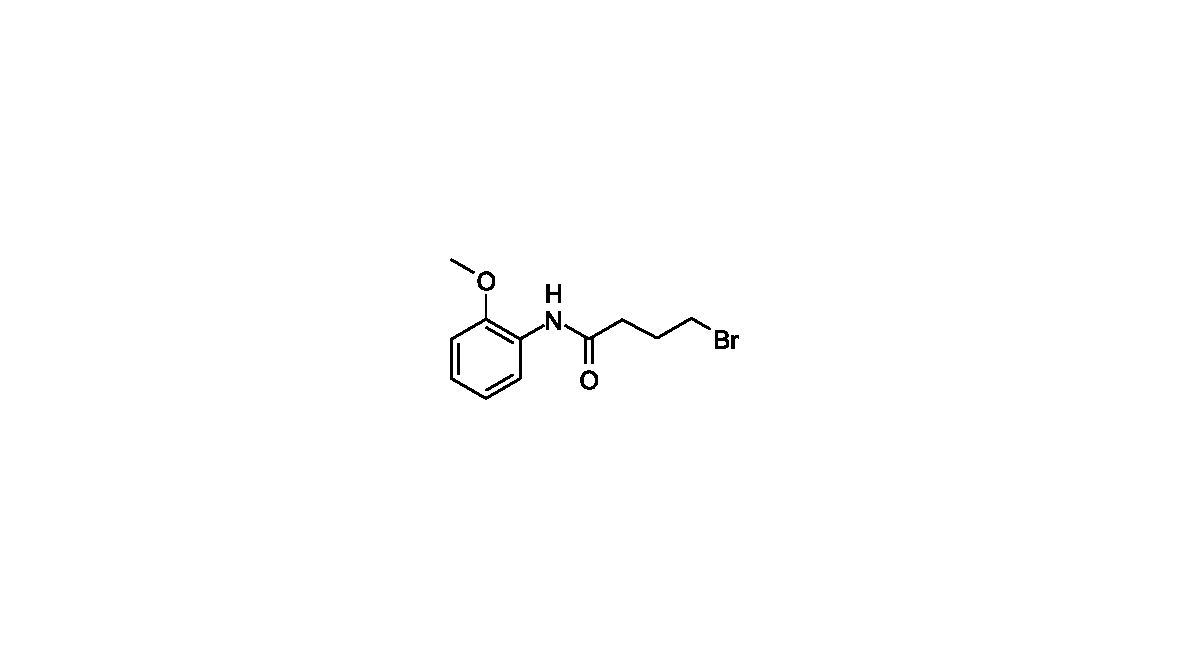
\includegraphics[scale=1]{2MeOA4Br.eps}
	\end{center}
\end{scheme}

2-Methoxyaniline \compound{cmpd:2MeOA} (9.12 ml, 10.0 g, 81.2 mmol, 1 eq.) and \ce{NaHCO3} (8.19 g, 97.4 mmol, 1.2 eq.) were dissolved in water (100 ml) and \ce{CH2Cl2} (100 ml). The mixture was cooled to 0 $^\circ$C and 4-bromobutyryl chloride \compound{cmpd:Cl4Br} (9.40 ml, 15.1 g, 81.2 mmol, 1 eq.) was added dropwise over 15 min. The mixture was stirred at 0 $^\circ$C for 1.5 h, then the aqueous layer was removed. The organic layer was dried with \ce{MgSO4} and purified by column chromatography (\ce{SiO2}, 5-25 \% EtOAc/P.E.). The combined pure fractions were dried with \ce{MgSO4} and evaporated under reduced pressure. \compound{cmpd:2MeOA4Br} was obtained as an initially colourless liquid which slowly turned blue then black if left out on the bench (11.0 g, 40.6 mmol, 50.0 \%).
\\[1\baselineskip]
\noindent{\textbf{TLC} \textit{R$_f$} = 0.16 (10 \% EtOAc/P.E.)}
\\[1\baselineskip]
\noindent{\textbf{IR} (neat) $\nu_{max}$ / cm$^{-1}$ = 
	3410.2 (N-H),
	3313.4 (N-H),
	2961.6 (C-H),
	2939.5 (C-H),
	2902.5 (C-H),
	%1770.9
	1676.4 (amide C=O)}
\\[1\baselineskip]
\noindent{\textbf{$^{1}$H NMR} (400 MHz, \ce{CDCl3} d$_1$) $\delta$ / ppm = 
	8.32 (dd, \textit{J} = 8.0, 1.7 Hz, 1 H, \textit{ortho} to NH), 
	7.85 (br s, 1 H, N\underline{H}), 
	7.02 (td, \textit{J} = 7.9, 1.7 Hz, 1 H, \textit{para} to NH), 
	6.93 (td, \textit{J} = 7.7, 1.4 Hz, 1 H, \textit{para} to OCH$_3$), 
	6.85 (dd, \textit{J} = 8.1, 1.5 Hz, 1 H, \textit{ortho} to OCH$_3$), 
	3.85 (s, 3 H, C\underline{H}$_3$), 
	3.50 (t, \textit{J} = 6.4 Hz, 2 H, C\underline{H}$_2$Br), 
	2.56 (t, \textit{J} = 7.1 Hz, 2 H, C(=O)C\underline{H}$_2$), 
	2.25 (quin, \textit{J} = 6.7 Hz, 2 H, C(=O)CH$_2$C\underline{H}$_2$)}
\\[1\baselineskip]
\noindent{\textbf{$^{13}$C NMR} (101 MHz, \ce{CDCl3} d$_1$) $\delta$ / ppm = 
	169.4 (\underline{C}(=O)), 
	147.6 (\textit{ipso} to OCH$_3$), 
	127.2 (\textit{ipso} to NH), 
	123.5 (\textit{para} to NH), 
	120.7 (\textit{para} to OCH$_3$), 
	119.6 (\textit{ortho} to NH and \textit{meta} to OCH$_3$), 
	109.8 (\textit{ortho} to OCH$_3$ and \textit{meta} to NH), 
	55.5 (\underline{C}H$_3$), 
	35.4 (C(=O)\underline{C}H$_2$), 
	33.1 (\underline{C}H$_2$Br), 
	27.9 (C(=O)CH$_2$\underline{C}H$_2$)}
\\[1\baselineskip]
\noindent{\textbf{HRMS} (ESI$^+$) \textit{m}/\textit{z} / Da = 272.0287, [M+H]$^+$ found, [\ce{C11H15BrNO2}]$^+$ requires 272.0286}
\\[1\baselineskip]
The compound has not been reported previously.



\subsection{Methyl 1\hyp{}cyclopropyl\hyp{}6\hyp{}fluoro\hyp{}7\hyp{}(4\hyp{}(4\hyp{}((2\hyp{}methoxyphenyl)amino)\hyp{}4\hyp{}oxobutyl)\allowbreak piperazin\hyp{}1\hyp{}yl)\hyp{}4\hyp{}oxo\hyp{}1,4\hyp{}dihydroquinoline\hyp{}3\hyp{}carboxylate \compound{cmpd:2MeOA4CipMe}}

%%LMO\hyp{}2\hyp{}030 (messy, possible mess up on amounts? Too much CipMe?), LMO\hyp{}2\hyp{}035 (forgot base until late, not sure if worked?), LMO\hyp{}2\hyp{}037 (??? didn't write down), LMO\hyp{}2\hyp{}038 (done but purification fail), LMO\hyp{}2\hyp{}039 (done?)

\begin{scheme}[H]
	\begin{center}
		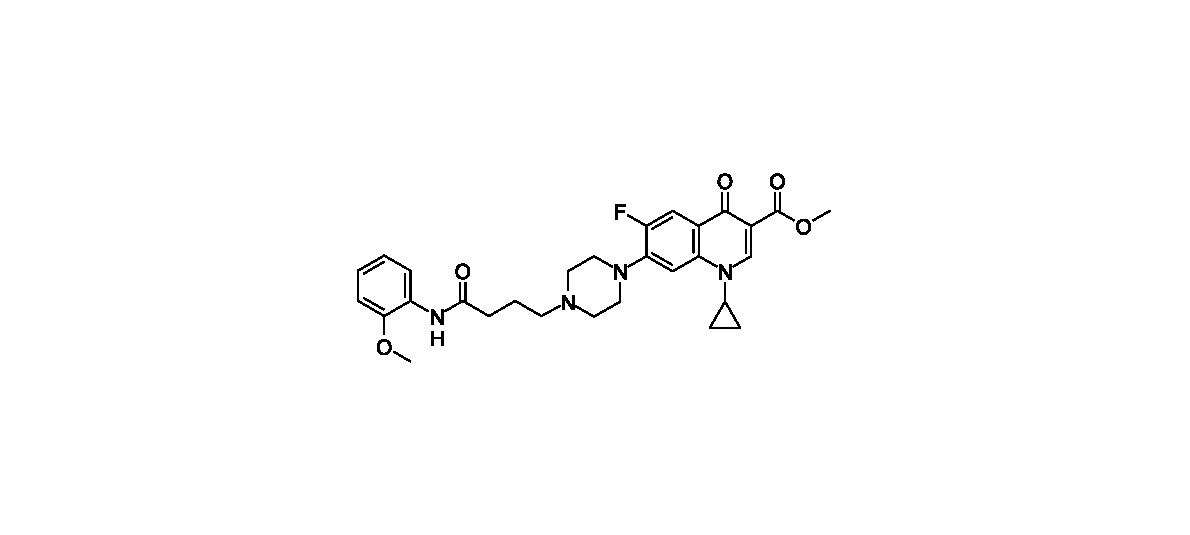
\includegraphics[scale=1]{2MeOA4CipMe.eps}
	\end{center}
\end{scheme}

Methyl 1\hyp{}cyclopropyl\hyp{}6\hyp{}fluoro\hyp{}4\hyp{}oxo\hyp{}7\hyp{}(piperazin\hyp{}1\hyp{}yl)\hyp{}1,4\hyp{}dihydroquinoline\hyp{}3\hyp{}carboxylate \compound{cmpd:CipMe} (500 mg, 1.45 mmol, 1 eq.), 4\hyp{}bromo\hyp{}\textit{N}\hyp{}(2\hyp{}methoxyphenyl)butanamide \compound{cmpd:2MeOA4Br} (788 mg, 2.90 mmol, 2 eq.), DIPEA (1.28 ml, 950 mg, 7.35 mmol, 5 eq.), \ce{NaI} (275 mg, 1.83 mmol, 1.3 eq.) and acetonitrile (10 ml) were stirred in a microwave reactor at 100 $^{\circ}$C for 4 h. The mixture was dry-loaded onto \ce{SiO2} and purified by column chromatography (\ce{SiO2}, 4 \% MeOH/\ce{CH2Cl2}). The combined pure fractions were dried with \ce{MgSO4} and evaporated under reduced pressure. \compound{cmpd:2MeOA4CipMe} was obtained as a bright pink glass (79.7 mg, 0.149 mmol, 10.2 \%).
\\[1\baselineskip]
\noindent{\textbf{TLC} \textit{R$_f$} = 0.40 (10 \% MeOH/\ce{CH2Cl2})}
\\[1\baselineskip]
\noindent{\textbf{IR} (neat) $\nu_{max}$ / cm$^{-1}$ = 
	2947.1 (C-H),
	2833.7 (C-H),
	1718.9 (ester C=O),
	1685.3 (amide C=O),
	1617.3 (quinolone C=O)}
\\[1\baselineskip]
\noindent{\textbf{$^{1}$H NMR} (400 MHz, \ce{CDCl3} d$_1$) $\delta$ / ppm = 
	8.48 (s, 1 H, \textit{ortho} to C(=O)OCH$_3$), 
	8.36 (d, \textit{J} = 7.9 Hz, 1 H, \textit{ortho} to NH), 
	7.87 - 7.99 (m, 2 H, \textit{ortho} to F and N\underline{H}), 
	7.19 (d, \textit{J} = 6.5 Hz, 1 H, \textit{meta} to F), 
	7.01 (t, \textit{J} = 7.5 Hz, 1 H, \textit{para} to NH), 
	6.93 (t, \textit{J} = 7.7 Hz, 1 H, \textit{para} to OCH$_3$), 
	6.85 (d, \textit{J} = 7.9 Hz, 1 H, \textit{ortho} to OCH$_3$), 
	3.88 (s, 3 H, C(=O)OC\underline{H}$_3$), 
	3.85 (s, 3 H, aromatic OC\underline{H}$_3$), 
	3.41 (tt, \textit{J} = 6.9, 4.0 Hz, 1 H, NC\underline{H}(CH$_2$)$_2$), 
	3.25 (br t, \textit{J} = 5.0, 5.0 Hz, 4 H, C(=O)CH$_2$CH$_2$CH$_2$N(CH$_2$C\underline{H}$_2$)CH$_2$C\underline{H}$_2$), 
	2.67 (br t, \textit{J} = 5.0, 5.0 Hz, 4 H, C(=O)CH$_2$CH$_2$CH$_2$N(C\underline{H}$_2$)C\underline{H}$_2$), 
	2.53 (t, \textit{J} = 7.0 Hz, 2 H, C(=O)CH$_2$CH$_2$C\underline{H}$_2$N), 
	2.47 (t, \textit{J} = 7.1 Hz, 2 H, C(=O)C\underline{H}$_2$CH$_2$CH$_2$N), 
	1.97 (quin, \textit{J} = 6.8 Hz, 2 H, C(=O)CH$_2$C\underline{H}$_2$CH$_2$N), 
	1.25 - 1.33 (m, 2 H, NCH(C\underline{H}H)$_2$), 
	1.07 - 1.14 (m, 2 H, NCH(CH\underline{H})$_2$)}
\\[1\baselineskip]
\noindent{\textbf{$^{13}$C NMR} (101 MHz, \ce{CDCl3} d$_1$) $\delta$ / ppm = 
	172.9 (\underline{C}(=O)CC(=O)OCH$_3$), 
	170.8 (NH\underline{C}(=O)), 
	166.2 (\underline{C}(=O)O\allowbreak CH$_3$), 
	153.3 (d, \textit{J} = 248.0 Hz, \textit{ipso} to F), 
	148.2 (\underline{C}=CC(=O)OCH$_3$), 
	147.6 (\textit{ipso} to OCH$_3$), 
	144.4 (d, \textit{J} = 10.4 Hz, \textit{ipso} to piperazine), 
	137.9 (\textit{para} to F), 
	127.6 (\textit{ipso} to NH), 
	123.4 (\textit{para} to NH), 
	122.7 (d, \textit{J} = 7.8 Hz, \textit{para} to piperazine), 
	121.0 (\textit{para} to OCH$_3$), 
	119.7 (\textit{ortho} to NH and \textit{meta} to OCH$_3$), 
	113.0 (d, \textit{J} = 22.5 Hz, \textit{ortho} to C=O and \textit{ortho} to F), 
	109.8 (\textit{ortho} to OCH$_3$ and \textit{meta} to NH, and \underline{C}C(=O)OCH$_3$), 
	104.7 (\textit{meta} to C=O and \textit{meta} to F), 
	57.2 (CH$_2$CH$_2$\underline{C}H$_2$N), 
	55.6 (aromatic O\underline{C}H$_3$), 
	52.7 (CH$_2$CH$_2$CH$_2$N(\underline{C}H$_2$)\underline{C}H$_2$), 
	51.9 (C(=O)O\underline{C}H$_3$), 
	49.8 (CH$_2$CH$_2$CH$_2$N(CH$_2$\underline{C}H$_2$)CH$_2$CH$_2$), 
	49.8 (CH$_2$CH$_2$CH$_2$N(CH$_2$CH$_2$)CH$_2$\underline{C}H$_2$), 
	35.5 (\underline{C}H$_2$\allowbreak CH$_2$CH$_2$N), 
	34.5 (N\underline{C}H(CH$_2$)$_2$), 
	22.3 (CH$_2$\underline{C}H$_2$CH$_2$N), 
	8.0 (NCH(\underline{C}H$_2$)$_2$)}
\\[1\baselineskip]
%\noindent{\textbf{$^{19}$F NMR} (376.45 MHz, \ce{CDCl3} d$_1$) $\delta$ / ppm = ??\todo{Check for F}}
%\\[1\baselineskip]
\noindent{\textbf{HRMS} (ESI$^+$) \textit{m}/\textit{z} / Da = 537.2523, [M+H]$^+$ found, [\ce{C29H34FN4O5}]$^+$ requires 537.2513}
\\[1\baselineskip]
The compound has not been reported previously.

\subsection{4\hyp{}Azido\hyp{}\textit{N}\hyp{}(2\hyp{}methoxyphenyl)butanamide \compound{cmpd:2MeOA4N3}}

%%LMO\hyp{}2\hyp{}032 (done), LMO\hyp{}2\hyp{}033 (big, done)
%2016-03-29 13.25.58.jpg

\begin{scheme}[H]
	\begin{center}
		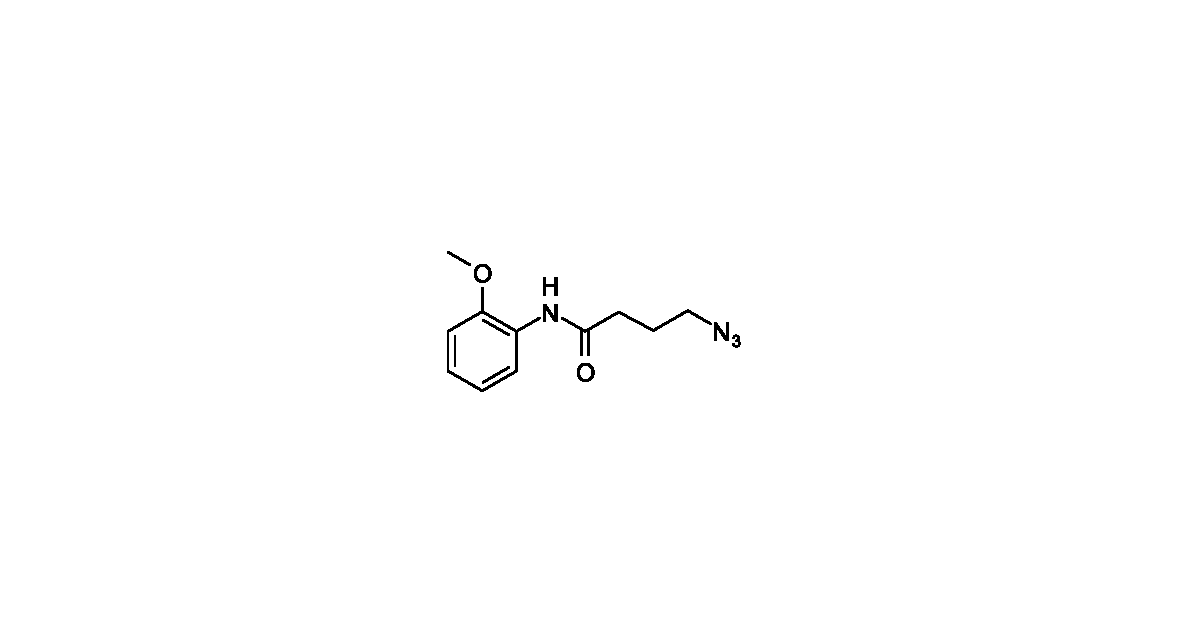
\includegraphics[scale=1]{2MeOA4N3.eps}
	\end{center}
\end{scheme}

4\hyp{}Bromo\hyp{}\textit{N}\hyp{}(2\hyp{}methoxyphenyl)butanamide \compound{cmpd:2MeOA4Br} (2.05 g, 7.51 mmol, 1 eq.) and \ce{NaN3} (1.17 g, 18.0 mmol, 2.4 eq.) were refluxed in acetonitrile (100 ml) for 2 h. The mixture was cooled and filtered, and the fitrate was dry-loaded onto \ce{SiO2} and purified by column chromatography using a Combiflash (\ce{SiO2}, 8-14 \% then hold at 14 \% EtOAc/P.E.). \compound{cmpd:2MeOA4N3} was obtained as an initially colourless liquid which slowly turned blue then black if left out on the bench (0.469 g, 2.00 mmol, 26.7 \%).
\\[1\baselineskip]
\noindent{\textbf{TLC} \textit{R$_f$} = 0.20 (25 \% EtOAc/P.E.)}
\\[1\baselineskip]
\noindent{\textbf{IR} (neat) $\nu_{max}$ / cm$^{-1}$ = 
	3419.7 (N-H),
	3329.6 (N-H),
	2094.8 (azide),
	1672.3 (amide C=O)}
\\[1\baselineskip]
\noindent{\textbf{$^{1}$H NMR} (400 MHz, \ce{CDCl3} d$_1$) $\delta$ / ppm = 
	8.32 (dd, \textit{J} = 7.9, 1.0 Hz, 1 H, \textit{ortho} to NH), 
	7.86 (br s, 1 H, N\underline{H}), 
	7.00 (td, \textit{J} = 7.5, 1.5 Hz, 1 H, \textit{para} to NH), 
	6.90 (td, \textit{J} = 7.7, 1.1 Hz, 1 H, \textit{para} to OCH$_3$), 
	6.83 (dd, \textit{J} = 8.1, 1.4 Hz, 1 H, \textit{ortho} to OCH$_3$), 
	3.81 (s, 3 H, C\underline{H}$_3$), 
	3.33 (t, \textit{J} = 6.7 Hz, 2 H, C\underline{H}$_2$Br), 
	2.42 (t, \textit{J} = 7.2 Hz, 2 H, C(=O)C\underline{H}$_2$), 
	1.94 (quin, \textit{J} = 6.9 Hz, 2 H, C(=O)CH$_2$C\underline{H}$_2$)}
\\[1\baselineskip]
\noindent{\textbf{$^{13}$C NMR} (101 MHz, \ce{CDCl3} d$_1$) $\delta$ / ppm = 
	169.5 (\underline{C}(=O)), 
	147.6 (\textit{ipso} to OCH$_3$), 
	127.1 (\textit{ipso} to NH), 
	123.4 (\textit{para} to NH), 
	120.5 (\textit{para} to OCH$_3$), 
	119.5 (\textit{ortho} to NH and \textit{meta} to OCH$_3$), 
	109.6 (\textit{ortho} to OCH$_3$ and \textit{meta} to NH), 
	55.2 (\underline{C}H$_3$), 
	50.3 (\underline{C}H$_2$N$_3$), 
	33.9 (C(=O)\underline{C}H$_2$), 
	24.3 (C(=O)CH$_2$\underline{C}H$_2$)}
\\[1\baselineskip]
\noindent{\textbf{HRMS} (ESI$^+$) \textit{m}/\textit{z} / Da = 257.1010, [M+H]$^+$ found, [\ce{C11H14N4NaO2}]$^+$ requires 257.1014}
\\[1\baselineskip]
The data are consistent with the literature\cite{Srinivasan2009}.

%(B4-4C). 4-Azido-N-(2-methoxy-phenyl)-butyramide.
%H- NMR (500 MHz, DMSO-d6) d 9.06 (s, 1H), 7.88–7.86 (m, 1H),
%7.03–6.97 (m, 2H), 6.86–6.83 (t, 1H), 3.8 (s, 3H), 3.35–3.32 (t, J = 6.92 Hz, 2H), 2.46–2.41 (m, 2H), 1.80–1.77 (m, 2H).
%C-NMR (125 MHz, DMSO-d6) d 170.41, 149.64, 127.23, 124.26, 122.13,
%120.09, 111.06, 55.55, 50.25, 32.94, 24.38. (B7-4C).

\subsection{1\hyp{}Cyclopropyl\hyp{}6\hyp{}fluoro\hyp{}7\hyp{}(4\hyp{}(4\hyp{}(1\hyp{}(4\hyp{}((2\hyp{}methoxyphenyl)amino)\hyp{}4\hyp{}oxobutyl)\hyp{}1\textit{H}\hyp{}1,2,3\hyp{}triazol\hyp{}4\hyp{}yl)\allowbreak butyl)piperazin\hyp{}1\hyp{}yl)\hyp{}4\hyp{}oxo\hyp{}1,4\hyp{}dihydroquinoline\hyp{}3\hyp{}car\allowbreak b\allowbreak oxylic acid \compound{cmpd:2MeOA4T4Cip}}

%%LMO\hyp{}2\hyp{}036 (done)
%2016-04-05

\begin{scheme}[H]
	\begin{center}
		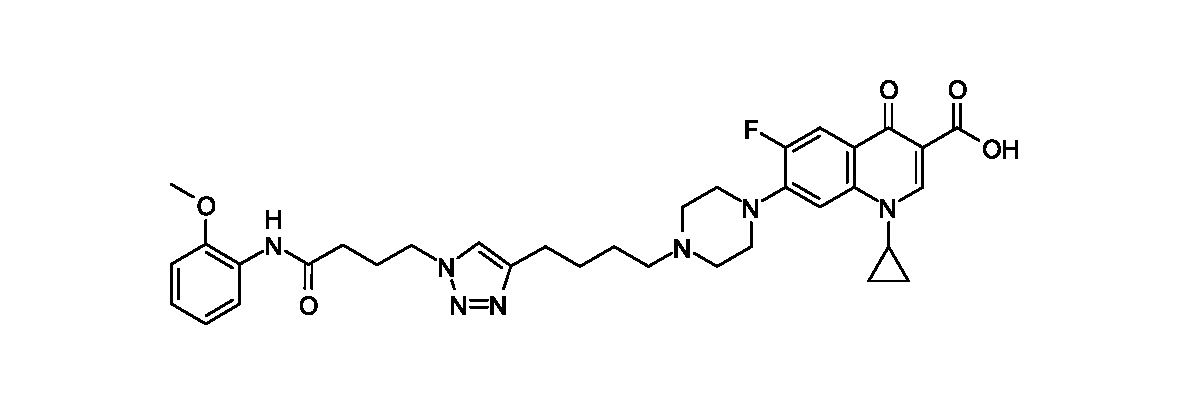
\includegraphics[scale=1]{2MeOA4T4Cip.eps}
	\end{center}
\end{scheme}

1-Cyclopropyl-6-fluoro-7-(4-(hex-5-yn-1-yl)piperazin-1-yl)-4-oxo-1,4\hyp{}dihydro\-quinoline-3-carboxylic acid \compound{cmpd:Y4Cip} (24.1 mg, 58.6 $\mu$mol, 1 eq.) and 4\hyp{}azido\hyp{}\textit{N}\hyp{}(2\hyp{}methoxyphenyl)butanamide \compound{cmpd:2MeOA4N3} (13.7 mg, 58.5 $\mu$mol, 1 eq.) were dissolved in water (3 ml), \textit{t}-BuOH (9 ml) and \ce{CH2Cl2} (9 ml), and the mixture was degassed by bubbling through \ce{N2}. A solution of \ce{CuSO4} and THPTA (117 $\mu$l, 5.85 $\mu$mol, 0.1 eq., 50 mM, aq.) was added, followed by a solution of sodium ascorbate (234 $\mu$l, 11.7 $\mu$mol, 0.2 eq., 50 mM, aq.). The mixture was stirred at room temperature under argon for 16 h. Water (25 ml), \ce{CH2Cl2} (25 ml) and MeOH (5 ml) were added and the organic layer was separated off, dry-loaded onto \ce{SiO2} and purified by column chromatography using a Combiflash (\ce{SiO2}, 3-23 \% MeOH/\ce{CH2Cl2}). The combined pure fractions were dried with \ce{MgSO4} and evaporated under reduced pressure. \compound{cmpd:2MeOA4T4Cip} was obtained as a clear glass (14.7 mg, 22.8 $\mu$mol, 39.0 \%).
\\[1\baselineskip]
\noindent{\textbf{TLC} \textit{R$_f$} = 0.28 (10 \% MeOH/\ce{CH2Cl2})}
\\[1\baselineskip]
%\noindent{\textbf{mp} \textit{T} / $^{\circ}$C = ?? (??)}
%\\[1\baselineskip]
\noindent{\textbf{IR} (neat) $\nu_{max}$ / cm$^{-1}$ = 
	2926.5 (C-H),
	2846.6 (C-H),
	1723.4 (carboxylic acid C=O),
	1682.0 (amide C=O),
	1625.8 (quinolone C=O),
	1612.8 (triazole)}
\\[1\baselineskip]
\noindent{\textbf{$^{1}$H NMR} (400 MHz, \ce{CDCl3}) $\delta$ / ppm = 
	15.05 (br s, 1 H, C(=O)O\underline{H}), 
	8.76 (s, 1 H, \textit{ortho} to C(=O)OH), 
	8.31 (dd, \textit{J} = 8.0, 1.7 Hz, 1 H, \textit{ortho} to NH), 
	8.00 (d, \textit{J} = 13.0 Hz, 1 H, \textit{ortho} to F), 
	7.83 (br s, 1 H, N\underline{H}), 
	7.37 (s, 1 H, C\underline{H}=CCH$_2$), 
	7.35 (d, \textit{J} = 7.2 Hz, 1 H, \textit{meta} to F), 
	7.04 (td, \textit{J} = 7.7, 1.7 Hz, 1 H, \textit{para} to NH), 
	6.95 (td, \textit{J} = 7.8, 1.5 Hz, 1 H, \textit{para} to OCH$_3$), 
	6.88 (dd, \textit{J} = 8.1, 1.4 Hz, 1 H, \textit{ortho} to OCH$_3$), 
	4.47 (t, \textit{J} = 6.7 Hz, 2 H, C(=O)CH$_2$CH$_2$C\underline{H}$_2$N), 
	3.88 (s, 3 H, C\underline{H}$_3$), 
	3.54 (tt, \textit{J} = 6.9, 4.0 Hz, 1 H, NC\underline{H}(CH$_2$)$_2$), 
	3.35 (br t, \textit{J} = 4.7 Hz, 4 H, CH=CCH$_2$CH$_2$CH$_2$CH$_2$N(CH$_2$C\underline{H}$_2$)CH$_2$C\underline{H}$_2$), 
	2.76 (t, \textit{J} = 7.5 Hz, 2 H, CH=C\underline{C}H$_2$), 
	2.66 (t, \textit{J} = 4.7 Hz, 4 H, CH=CCH$_2$CH$_2$CH$_2$CH$_2$N(C\underline{H}$_2$)C\underline{H}$_2$), 
	2.47 (t, \textit{J} = 7.3 Hz, 2 H, CH=CCH$_2$CH$_2$CH$_2$C\underline{H}$_2$N), 
	2.44 (t, \textit{J} = 6.8 Hz, 2 H, C(=O)C\underline{H}$_2$CH$_2$CH$_2$N), 
	2.32 (quin, \textit{J} = 6.7 Hz, 2 H, C(=O)CH$_2$C\underline{H}$_2$CH$_2$N), 
	1.75 (quin, \textit{J} = 7.6 Hz, 2 H, CH=CCH$_2$C\underline{H}$_2$CH$_2$CH$_2$N), 
	1.61 (quin, \textit{J} = 7.5 Hz, 2 H, CH=CCH$_2$CH$_2$C\underline{H}$_2$CH$_2$N), 
	1.35 - 1.42 (m, 2 H, NCH(C\underline{H}H)$_2$), 
	1.17 - 1.22 (m, 2 H, NCH(CH\underline{H})$_2$)}
\\[1\baselineskip]
\noindent{\textbf{$^{13}$C NMR} (101 MHz, \ce{CDCl3}) $\delta$ / ppm = 
	177.1 (\underline{C}(=O)CC(=O)OH), 
	169.5 (NH\underline{C}(=O)), 
	167.0 (\underline{C}(=O)OH), 
	153.7 (d, \textit{J} = 251.4 Hz, \textit{ipso} to F), 
	148.1 (CH=\underline{C}CH$_2$), 
	147.8 (\textit{ipso} to OCH$_3$), 
	147.3 (\underline{C}=CC(=O)OH), 
	145.9 (d, \textit{J} = 10.4 Hz, \textit{ipso} to piperazine), 
	139.1 (\textit{para} to F), 
	127.3 (\textit{ipso} to NH), 
	123.9 (\textit{para} to NH), 
	121.0 (\textit{para} to OCH$_3$), 
	120.9 (\underline{C}H=CCH$_2$), 
	119.7 (\textit{para} to piperazine, and \textit{ortho} to NH and \textit{meta} to OCH$_3$), 
	112.4 (d, \textit{J} = 23.4 Hz, \textit{ortho} to C=O and \textit{ortho} to F), 
	109.9 (\textit{ortho} to OCH$_3$ and \textit{meta} to NH), 
	108.1 (\underline{C}C(=O)OH), 
	104.7 (\textit{meta} to C=O and \textit{meta} to F), 
	58.1 (CH=CCH$_2$CH$_2$CH$_2$\underline{C}H$_2$N), 
	55.6 (\underline{C}H$_3$), 
	52.8 (CH=CCH$_2$CH$_2$CH$_2$CH$_2$N(\underline{C}H$_2$)\underline{C}H$_2$), 
	49.8 (CH=CCH$_2$CH$_2$CH$_2$CH$_2$N(CH$_2$\underline{C}H$_2$)CH$_2$CH$_2$), 
	49.8 (CH=CCH$_2$CH$_2$CH$_2$CH$_2$N(CH$_2$CH$_2$)CH$_2$\underline{C}H$_2$), 
	49.1 (C(=O)CH$_2$CH$_2$\underline{C}H$_2$N), 
	35.2 (N\underline{C}H(CH$_2$)$_2$), 
	33.8 (C(=O)\underline{C}H$_2$CH$_2$CH$_2$N), 
	27.3 (CH=CCH$_2$\underline{C}H$_2$CH$_2$CH$_2$N), 
	26.4 (CH=CCH$_2$CH$_2$\underline{C}H$_2$CH$_2$N), 
	26.0 (C(=O)CH$_2$\underline{C}H$_2$CH$_2$N), 
	25.5 (CH=C\underline{C}H$_2$CH$_2$CH$_2$CH$_2$N), 
	8.2 (NCH\allowbreak (\underline{C}H$_2$)$_2$)}
\\[1\baselineskip]
\noindent{\textbf{$^{19}$F NMR} (376.45 MHz, \ce{CDCl3}) $\delta$ / ppm = 
	-120.7 (s, ciprofloxacin F)}
\\[1\baselineskip]
\noindent{\textbf{HRMS} (ESI$^+$) \textit{m}/\textit{z} / Da = 646.3132, [M+H]$^+$ found, [\ce{C34H41FN7O5}]$^+$ requires 646.3153}
\\[1\baselineskip]
The compound has not been reported previously.

\subsection{4\hyp{}Bromo\hyp{}\textit{N}\hyp{}(3\hyp{}methoxyphenyl)butanamide \compound{cmpd:3MeOA4Br}}

%%LMO\hyp{}2\hyp{}029 (done)
%2016-04-13

\begin{scheme}[H]
	\begin{center}
		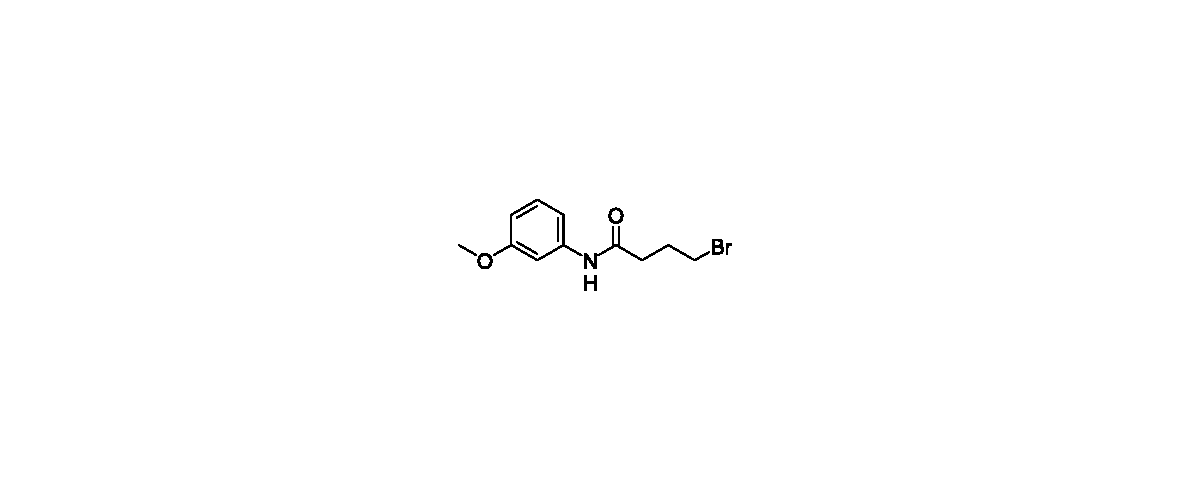
\includegraphics[scale=1]{3MeOA4Br.eps}
	\end{center}
\end{scheme}

3-Methoxyaniline \compound{cmpd:3MeOA} (3.04 ml, 3.33 g, 27.1 mmol, 1 eq.) and \ce{NaHCO3} (2.73 g, 32.5 mmol, 1.2 eq.) were dissolved in water (30 ml) and \ce{CH2Cl2} (30 ml). The mixture was cooled to 0 $^\circ$C and 4-bromobutyryl chloride \compound{cmpd:Cl4Br} (3.13 ml, 5.03 g, 27.1 mmol, 1 eq.) was added dropwise over 5 min. The mixture was stirred at 0 $^\circ$C for 1 h, then the aqueous layer was removed. The organic layer was dry-loaded onto \ce{SiO2} and purified by column chromatography using a Combiflash (\ce{SiO2}, 0-100 \% EtOAc/P.E.). The combined pure fractions were dried with \ce{MgSO4} and evaporated under reduced pressure. \compound{cmpd:3MeOA4Br} was obtained as a pale pink amorphous solid (3.66 g, 13.5 mmol, 49.6 \%). %this is very contaminated now, by IR and mp... gone to p brown gooey crystals
\\[1\baselineskip]
\noindent{\textbf{TLC} \textit{R$_f$} = 0.18 (25 \% EtOAc/P.E.)}
\\[1\baselineskip]
%\noindent{\textbf{mp} \textit{T} / $^{\circ}$C = ?? (??)}
%\\[1\baselineskip]
\noindent{\textbf{IR} (neat) $\nu_{max}$ / cm$^{-1}$ = 
	1670.9 (amide C=O)}
\\[1\baselineskip]
\noindent{\textbf{$^{1}$H NMR} (400 MHz, \ce{CDCl3} d$_1$) $\delta$ / ppm = 
	8.45 (s, 1 H, N\underline{H}), 
	7.27 (t, \textit{J} = 2.2 Hz, 1 H, \textit{ortho} to OCH$_3$ and \textit{ortho} to NH), 
	7.14 (t, \textit{J} = 8.1 Hz, 1 H, \textit{meta} to OCH$_3$ and \textit{meta} to NH), 
	7.02 (d, \textit{J} = 8.3 Hz, 1 H, \textit{para} to OCH$_3$), 
	6.62 (dd, \textit{J} = 8.2, 2.1 Hz, 1 H, \textit{para} to NH), 
	3.71 (s, 3 H, C\underline{H}$_3$), 
	3.42 (t, \textit{J} = 6.5 Hz, 2 H, C\underline{H}$_2$Br), 
	2.51 (t, \textit{J} = 6.9 Hz, 2 H, C(=O)C\underline{H}$_2$), 
	2.19 (quin, \textit{J} = 6.8 Hz, 2 H, C(=O)CH$_2$C\underline{H}$_2$)}
\\[1\baselineskip]
\noindent{\textbf{$^{13}$C NMR} (101 MHz, \ce{CDCl3} d$_1$) $\delta$ / ppm = 
	170.3 (\underline{C}(=O)), 
	159.9 (\textit{ipso} to OCH$_3$), 
	139.0 (\textit{ipso} to NH), 
	129.5 (\textit{meta} to OCH$_3$ and \textit{meta} to NH), 
	112.1 (\textit{para} to OCH$_3$), 
	109.9 (\textit{para} to NH), 
	105.7 (\textit{ortho} to OCH$_3$ and \textit{ortho} to NH), 
	55.2 (\underline{C}H$_3$), 
	35.3 (C(=O)\underline{C}H$_2$), 
	33.2 (\underline{C}H$_2$Br), 
	28.0 (C(=O)CH$_2$\underline{C}H$_2$)}
\\[1\baselineskip]
\noindent{\textbf{HRMS} (ESI$^+$) The compound does not ionise.}
\\[1\baselineskip]
The compound has not been reported previously.







\subsection{Methyl 1\hyp{}cyclopropyl\hyp{}6\hyp{}fluoro\hyp{}7\hyp{}(4\hyp{}(4\hyp{}((3\hyp{}methoxyphenyl)amino)\hyp{}4\hyp{}oxobutyl)\allowbreak piperazin\hyp{}1\hyp{}yl)\hyp{}4\hyp{}oxo\hyp{}1,4\hyp{}dihydroquinoline\hyp{}3\hyp{}carboxylate \compound{cmpd:3MeOA4CipMe}}

%%LMO\hyp{}2\hyp{}041 (done)

\begin{scheme}[H]
	\begin{center}
		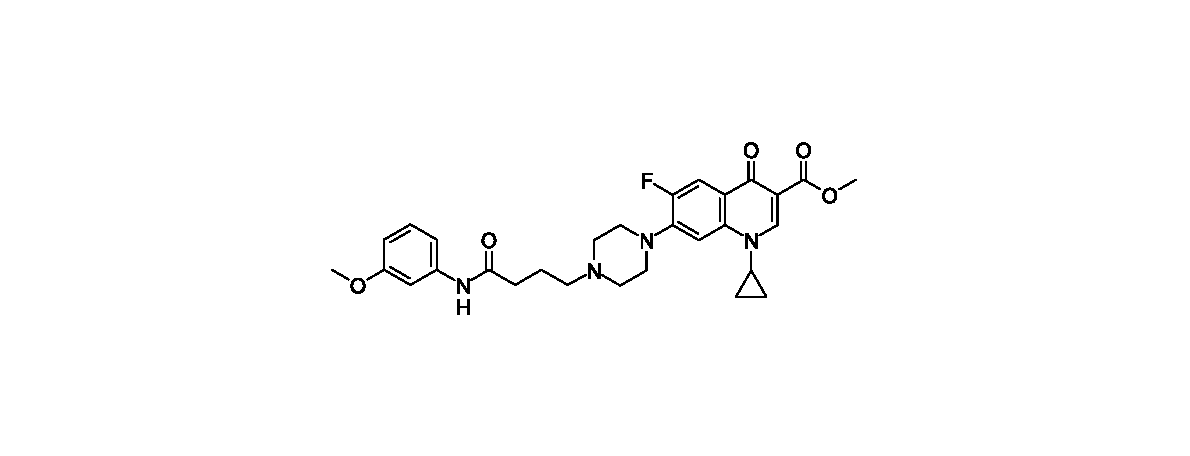
\includegraphics[scale=1]{3MeOA4CipMe.eps}
	\end{center}
\end{scheme}

Methyl 1\hyp{}cyclopropyl\hyp{}6\hyp{}fluoro\hyp{}4\hyp{}oxo\hyp{}7\hyp{}(piperazin\hyp{}1\hyp{}yl)\hyp{}1,4\hyp{}dihydroquinoline\hyp{}3\hyp{}carboxylate \compound{cmpd:CipMe} (500 mg, 1.45 mmol, 1 eq.), 4\hyp{}bromo\hyp{}\textit{N}\hyp{}(3\hyp{}methoxyphenyl)butanamide \compound{cmpd:3MeOA4Br} (788 mg, 2.90 mmol, 2 eq.), DIPEA (1.28 ml, 950 mg, 7.35 mmol, 5 eq.), \ce{NaI} (275 mg, 1.83 mmol, 1.3 eq.) and acetonitrile (10 ml) were stirred in a microwave reactor at 100 $^{\circ}$C for 4 h. The mixture was evaporated under reduced pressure and partitioned between \ce{CH2Cl2} (50 ml) and water (50 ml). The organic layer was separated off and the aqueous layer was extracted again with \ce{CH2Cl2} (50 ml). The combined organic layers were dried with \ce{MgSO4} and purified by column chromatography (\ce{SiO2}, 0-4 \% MeOH/\ce{CH2Cl2}). The combined pure fractions were dried with \ce{MgSO4} and evaporated under reduced pressure. \compound{cmpd:3MeOA4CipMe} was obtained as an off-white amorphous solid (81.7 mg, 0.152 mmol, 10.5 \%).
\\[1\baselineskip]
\noindent{\textbf{TLC} \textit{R$_f$} = 0.38 (10 \% MeOH/\ce{CH2Cl2})}
\\[1\baselineskip]
%\noindent{\textbf{mp} \textit{T} / $^{\circ}$C = ?? (??)}
%\\[1\baselineskip]
\noindent{\textbf{IR} (neat) $\nu_{max}$ / cm$^{-1}$ = 
	3270.8 (amide N-H)
	2943.8 (C-H),
	2817.0 (C-H),
	1729.5 (ester C=O),
	%1699.2 \todo{what is this??}
	1682.0 (amide C=O),
	1613.5 (quinolone C=O)}
\\[1\baselineskip]
\noindent{\textbf{$^{1}$H NMR} (400 MHz, \ce{CDCl3}) $\delta$ / ppm = 
	8.56 (s, 1 H, \textit{ortho} to C(=O)OCH$_3$), 
	8.06 (d, \textit{J} = 13.3 Hz, 1 H, \textit{ortho} to F), 
	8.02 (br s, 1 H, N\underline{H}), 
	7.34 (t, \textit{J} = 1.7 Hz, 1 H, \textit{ortho} to OCH$_3$ and \textit{ortho} to NH), 
	7.25 (d, \textit{J} = 7.0 Hz, 1 H, \textit{meta} to F), 
	7.20 (t, \textit{J} = 8.2 Hz, 1 H, \textit{meta} to OCH$_3$ and \textit{meta} to NH), 
	6.98 (dd, \textit{J} = 7.8, 1.7 Hz, 1 H, \textit{para} to OCH$_3$), 
	6.65 (dd, \textit{J} = 8.2, 2.1 Hz, 1 H, \textit{para} to NH), 
	3.93 (s, 3 H, C(=O)OC\underline{H}$_3$), 
	3.80 (s, 3 H, aromatic OC\underline{H}$_3$), 
	3.42 (tt, \textit{J} = 6.8, 3.7 Hz, 1 H, NC\underline{H}(CH$_2$)$_2$), 
	3.31 (br t, \textit{J} = 4.3, 4.3 Hz, 4 H, C(=O)CH$_2$CH$_2$CH$_2$N(CH$_2$C\underline{H}$_2$)CH$_2$C\underline{H}$_2$), 
	2.73 (br t, \textit{J} = 4.5, 4.5 Hz, 4 H, C(=O)CH$_2$CH$_2$CH$_2$N(C\underline{H}$_2$)C\underline{H}$_2$), 
	2.58 (t, \textit{J} = 6.5 Hz, 2 H, C(=O)CH$_2$CH$_2$C\underline{H}$_2$N), 
	2.48 (t, \textit{J} = 6.8 Hz, 2 H, C(=O)C\underline{H}$_2$CH$_2$CH$_2$N), 
	2.00 (quin, \textit{J} = 6.8 Hz, 2 H, C(=O)CH$_2$C\underline{H}$_2$CH$_2$N), 
	1.29 - 1.36 (m, 2 H, NCH(C\underline{H}H)$_2$), 
	1.11 - 1.17 (m, 2 H, NCH(CH\underline{H})$_2$)}
\\[1\baselineskip]
\noindent{\textbf{$^{13}$C NMR} (101 MHz, \ce{CDCl3}) $\delta$ / ppm = 
	173.1 (\underline{C}(=O)CC(=O)OCH$_3$), 
	170.9 (NH\underline{C}(=O)), 
	166.3 (\underline{C}(=O)O\allowbreak CH$_3$), 
	160.1 (\textit{ipso} to OCH$_3$), 
	153.3 (d, J=250.1 Hz, \textit{ipso} to F), 
	148.4 (\underline{C}=CC(=O)OCH$_3$), 
	144.1 (d, J=10.1 Hz, \textit{ipso} to piperazine), 
	139.4 (\textit{ipso} to NH), 
	138.0 (\textit{para} to F), 
	129.6 (\textit{meta} to NH and \textit{meta} to OCH$_3$), 
	123.3 (d, J=6.4 Hz, \textit{para} to piperazine), 
	113.4 (d, J=23.3 Hz, \textit{ortho} to C=O and \textit{ortho} to F), 
	111.8 (\textit{para} to OCH$_3$), 
	110.0 (\underline{C}C(=O)OCH$_3$), 
	109.8 (\textit{para} to NH), 
	105.5 (\textit{ortho} to OCH$_3$ and \textit{ortho} to NH), 
	105.0 (\textit{meta} to C=O and \textit{meta} to F), 
	57.0 (CH$_2$CH$_2$\underline{C}H$_2$N), 
	55.3 (aromatic O\underline{C}H$_3$), 
	52.6 (CH$_2$CH$_2$CH$_2$N(\underline{C}H$_2$)\underline{C}H$_2$), 
	52.1 (C(=O)O\underline{C}H$_3$), 
	49.2 (CH$_2$CH$_2$CH$_2$N(CH$_2$\underline{C}H$_2$)CH$_2$\underline{C}H$_2$), 
	35.2 (\underline{C}H$_2$CH$_2$CH$_2$N), 
	34.6 (N\underline{C}H(CH$_2$)$_2$), 
	21.7 (CH$_2$\underline{C}H$_2$CH$_2$N), 
	8.2 (NCH(\underline{C}H$_2$)$_2$)}
\\[1\baselineskip]
\noindent{\textbf{$^{19}$F NMR} (376.45 MHz, MeOD) $\delta$ / ppm = 	
	-123.5 (s, ciprofloxacin F)}
\\[1\baselineskip]
\noindent{\textbf{HRMS} (ESI$^+$) \textit{m}/\textit{z} / Da = 537.2500, [M+H]$^+$ found, [\ce{C29H34FN4O5}]$^+$ requires 537.2513}
\\[1\baselineskip]
The compound has not been reported previously.


%\subsection{1\hyp{}cyclopropyl\hyp{}6\hyp{}fluoro\hyp{}7\hyp{}(4\hyp{}(4\hyp{}((2\hyp{}methoxyphenyl)amino)\hyp{}4\hyp{}oxobutyl)piperaz\hyp{}in\hyp{}1\hyp{}yl)\hyp{}4\hyp{}oxo\hyp{}1,4\hyp{}dihydroquinoline\hyp{}3\hyp{}carboxylate \compound{cmpd:2MeOA4Cip}}
%
%%%LMO\hyp{}2\hyp{}031 (from Cip, messy)
%
%\begin{scheme}[H]
%	\begin{center}
%		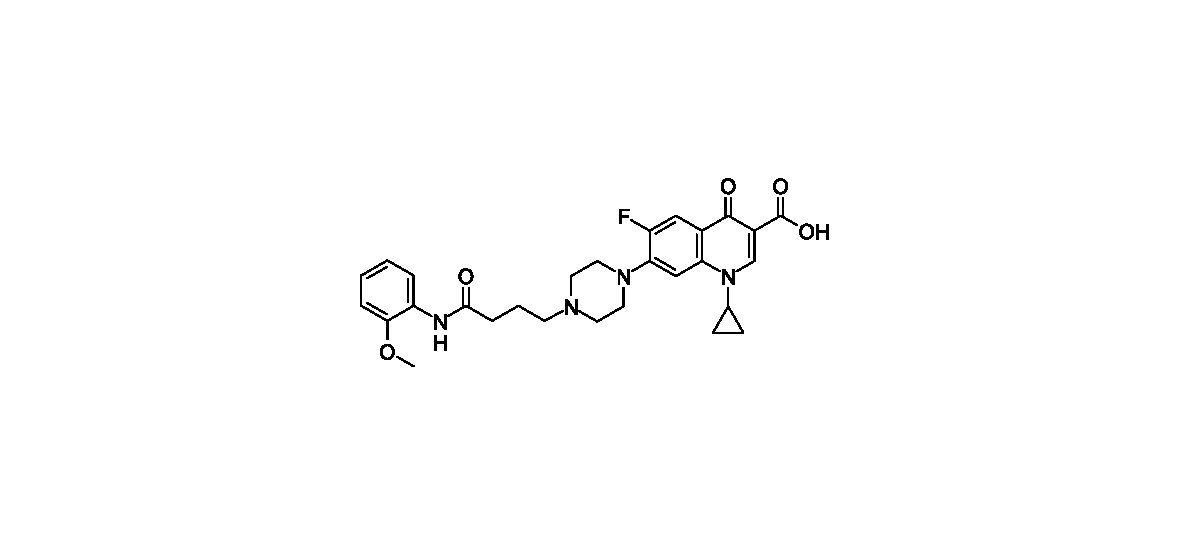
\includegraphics[scale=1]{2MeOA4Cip.eps}
%	\end{center}
%\end{scheme}
%
%\subsection{1\hyp{}cyclopropyl\hyp{}6\hyp{}fluoro\hyp{}7\hyp{}(4\hyp{}(4\hyp{}((3\hyp{}methoxyphenyl)amino)\hyp{}4\hyp{}oxobutyl)piperaz\hyp{}in\hyp{}1\hyp{}yl)\hyp{}4\hyp{}oxo\hyp{}1,4\hyp{}dihydroquinoline\hyp{}3\hyp{}carboxylate \compound{cmpd:3MeOA4Cip}}
%
%%%LMO\hyp{}2\hyp{}045 (by hydrolysis, done)
%
%\begin{scheme}[H]
%	\begin{center}
%		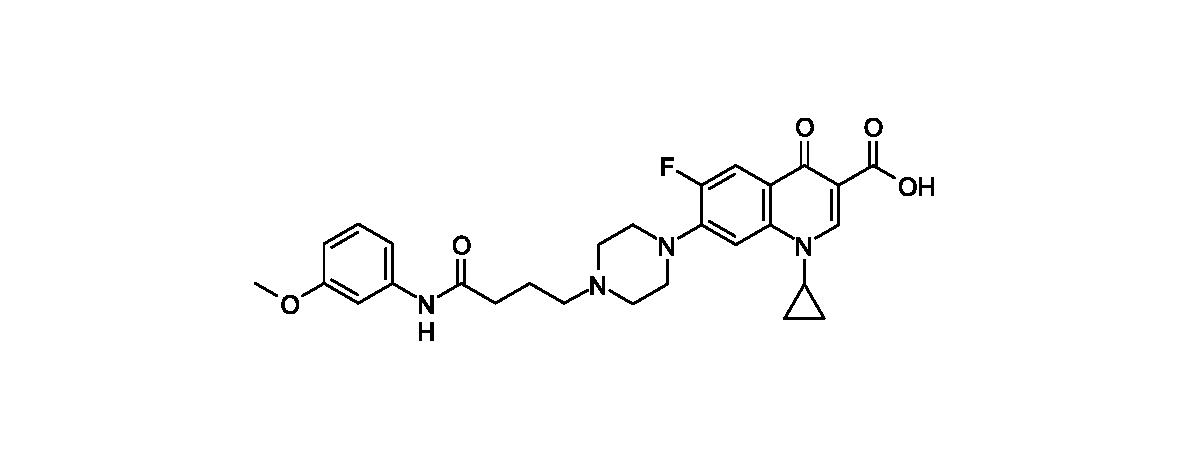
\includegraphics[scale=1]{3MeOA4Cip.eps}
%	\end{center}
%\end{scheme}
%
%Messy NMR, don't bother

\subsection{4\hyp{}Azido\hyp{}\textit{N}\hyp{}(3\hyp{}methoxyphenyl)butanamide \compound{cmpd:3MeOA4N3}}

%%LMO\hyp{}2\hyp{}040 (big, done)

\begin{scheme}[H]
	\begin{center}
		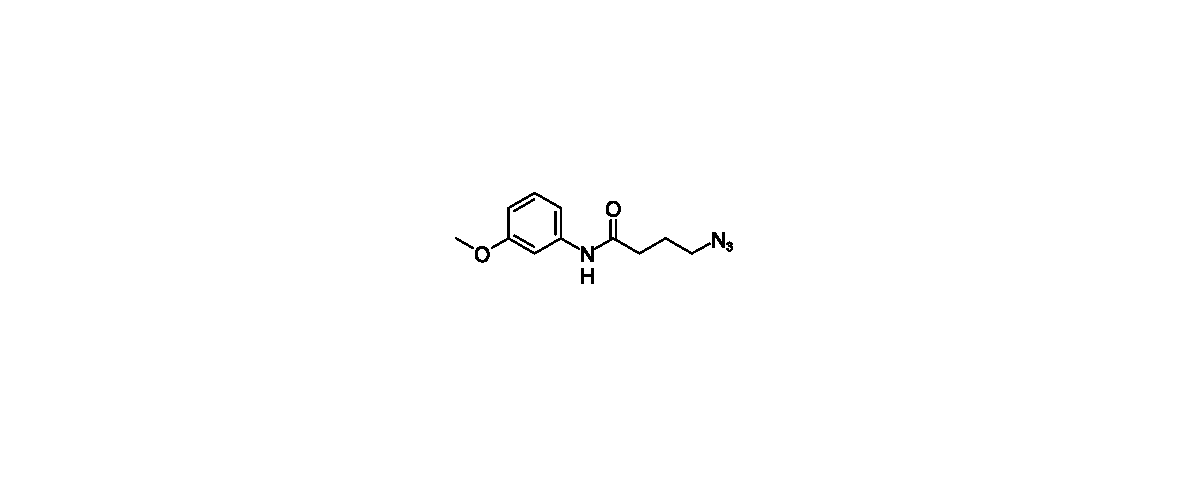
\includegraphics[scale=1]{3MeOA4N3.eps}
	\end{center}
\end{scheme}

4\hyp{}Bromo\hyp{}\textit{N}\hyp{}(3\hyp{}methoxyphenyl)butanamide \compound{cmpd:3MeOA4Br} (2.05 g, 7.51 mmol, 1 eq.) and \ce{NaN3} (1.17 g, 18.0 mmol, 2.4 eq.) were refluxed in acetonitrile (100 ml) for 7 h. The mixture was cooled and filtered, and the fitrate was dry-loaded onto \ce{SiO2} and purified by column chromatography using a Combiflash (\ce{SiO2}, 0-100 \% EtOAc/P.E.). The combined pure fractions were dried with \ce{MgSO4} and evaporated under reduced pressure. \compound{cmpd:3MeOA4N3} was obtained as an straw-coloured liquid (0.294 g, 1.25 mmol, 16.7 \%).
\\[1\baselineskip]
\noindent{\textbf{TLC} \textit{R$_f$} = 0.37 (50 \% EtOAc/P.E.)}
\\[1\baselineskip]
\noindent{\textbf{IR} (neat) $\nu_{max}$ / cm$^{-1}$ = 
	3298.3 (N-H),
	2094.7 (azide),
	1661.7 (amide C=O)}
\\[1\baselineskip]
\noindent{\textbf{$^{1}$H NMR} (400 MHz, MeOD) $\delta$ / ppm = 
	8.63 (br s, 1 H, N\underline{H}), 
	7.26 (t, \textit{J} = 2.3 Hz, 1 H, \textit{ortho} to OCH$_3$ and \textit{ortho} to NH), 
	7.15 (t, \textit{J} = 8.1 Hz, 1 H, \textit{meta} to OCH$_3$ and \textit{meta} to NH), 
	7.01 (dd, \textit{J} = 7.8, 1.6 Hz, 1 H, \textit{para} to OCH$_3$), 
	6.63 (dd, \textit{J} = 8.2, 1.9 Hz, 1 H, \textit{para} to NH), 
	3.69 (s, 3 H, C\underline{H}$_3$), 
	3.28 (t, \textit{J} = 6.7 Hz, 2 H, C\underline{H}$_2$N$_3$), 
	2.39 (t, \textit{J} = 7.4 Hz, 2 H, C(=O)C\underline{H}$_2$), 
	1.91 (quin, \textit{J} = 7.0 Hz, 2 H, C(=O)CH$_2$C\underline{H}$_2$)}
\\[1\baselineskip]
\noindent{\textbf{$^{13}$C NMR} (101 MHz, MeOD) $\delta$ / ppm = 
	170.8 (\underline{C}(=O)), 
	159.6 (\textit{ipso} to OCH$_3$), 
	138.9 (\textit{ipso} to NH), 
	129.2 (\textit{meta} to OCH$_3$ and \textit{meta} to NH), 
	112.3 (\textit{para} to OCH$_3$), 
	109.5 (\textit{para} to NH), 
	106.0 (\textit{ortho} to OCH$_3$ and \textit{ortho} to NH), 
	54.8 (\underline{C}H$_3$), 
	50.4 (\underline{C}H$_2$N$_3$), 
	33.6 (C(=O)\underline{C}H$_2$), 
	24.4 (C(=O)CH$_2$\underline{C}H$_2$)}
\\[1\baselineskip]
\noindent{\textbf{HRMS} (ESI$^+$) The compound does not ionise.}
\\[1\baselineskip]
The compound has not been reported previously.

\subsection{1\hyp{}Cyclopropyl\hyp{}6\hyp{}fluoro\hyp{}7\hyp{}(4\hyp{}(4\hyp{}(1\hyp{}(4\hyp{}((3\hyp{}methoxyphenyl)amino)\hyp{}4\hyp{}oxobutyl)\hyp{}1\textit{H}\hyp{}1,2,3\hyp{}triazol\hyp{}4\hyp{}yl)\allowbreak butyl)piperazin\hyp{}1\hyp{}yl)\hyp{}4\hyp{}oxo\hyp{}1,4\hyp{}dihydroquinoline\hyp{}3\hyp{}car\allowbreak b\allowbreak oxylic acid \compound{cmpd:3MeOA4T4Cip}}

%%LMO\hyp{}2\hyp{}043 (done)

\begin{scheme}[H]
	\begin{center}
		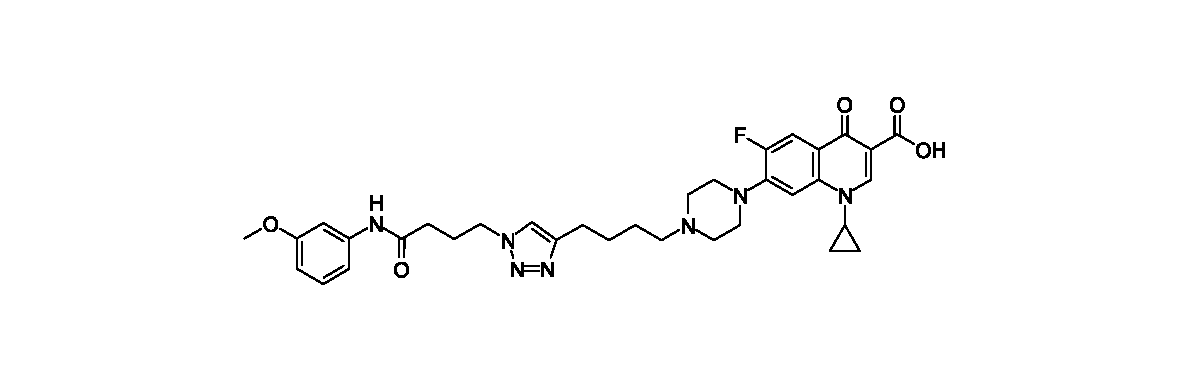
\includegraphics[scale=1]{3MeOA4T4Cip.eps}
	\end{center}
\end{scheme}

1-Cyclopropyl-6-fluoro-7-(4-(hex-5-yn-1-yl)piperazin-1-yl)-4-oxo-1,4\hyp{}dihydro\-quinoline-3-carboxylic acid \compound{cmpd:Y4Cip} \allowbreak (24.1 mg, 58.6 $\mu$mol, 1 eq.) and 4\hyp{}azido\hyp{}\textit{N}\hyp{}(3\hyp{}methoxyphenyl)butanamide \compound{cmpd:3MeOA4N3} (13.7 mg, 58.5 $\mu$mol, 1 eq.) were dissolved in water (1 ml), \textit{t}-BuOH (9 ml) and \ce{CH2Cl2} (10 ml), and the mixture was degassed by bubbling through \ce{N2}. A solution of \ce{CuSO4} and THPTA (58.5 $\mu$l, 5.85 $\mu$mol, 0.1 eq. 100 mM, aq.) was added, followed by a solution of sodium ascorbate (117 $\mu$l, 11.7 $\mu$mol, 0.2 eq., 100 mM, aq.). The mixture was stirred at room temperature under argon for 2 h, then the solvent was removed under reduced pressure. The resudue was partitioned between water (15 ml) and \ce{CH2Cl2} (15 ml), and the aqueous layer was extracted a further four times with \ce{CH2Cl2} (4$\times$15 ml). The combined organic layers were dried with \ce{MgSO4}, dry-loaded onto \ce{SiO2} and purified by column chromatography (\ce{SiO2}, 0-10 \% MeOH/\ce{CH2Cl2}). The combined pure fractions were dried with \ce{MgSO4} and evaporated under reduced pressure. \compound{cmpd:3MeOA4T4Cip} was obtained as a clear glass (1.9 mg, 2.9 $\mu$mol, 5.0 \%).
\\[1\baselineskip]
\noindent{\textbf{TLC} \textit{R$_f$} = 0.22 (10 \% MeOH/\ce{CH2Cl2})}
\\[1\baselineskip]
%\noindent{\textbf{mp} \textit{T} / $^{\circ}$C = ?? (??)}
%\\[1\baselineskip]
\noindent{\textbf{IR} (neat) $\nu_{max}$ / cm$^{-1}$ = 
	2922.8 (C-H),
	2849.5 (C-H),
	1725.8 (carboxylic acid C=O),
	1684.7 (amide C=O),
	1624.5 (quinolone C=O),
	1612.2 (triazole)}
\\[1\baselineskip]
\noindent{\textbf{$^{1}$H NMR} (400 MHz, DMSO d$_6$) $\delta$ / ppm = 
	15.23 (br s, 1 H, C(=O)O\underline{H}), 
	9.89 (s, 1 H, N\underline{H}), 
	8.66 (s, 1 H, \textit{ortho} to C(=O)OH), 
	7.90 (d, \textit{J} = 13.4 Hz, 1 H, \textit{ortho} to F), 
	7.88 (s, 1 H, C\underline{H}=CCH$_2$), 
	7.55 (d, \textit{J} = 7.6 Hz, 1 H, \textit{meta} to F), 
	7.27 (t, \textit{J} = 2.1 Hz, 1 H, \textit{ortho} to C=O and \textit{ortho} to F), 
	7.16 (t, \textit{J} = 8.1 Hz, 1 H, \textit{meta} to OCH$_3$ and \textit{meta} to NH), 
	7.08 (d, \textit{J} = 7.8 Hz, 1 H, \textit{para} to OCH$_3$), 
	6.59 (ddd, \textit{J} = 8.1, 2.4, 0.7 Hz, 1 H, \textit{para} to NH), 
	4.36 (t, \textit{J} = 6.9 Hz, 2 H, C(=O)CH$_2$CH$_2$C\underline{H}$_2$N), 
	3.81 (tt, \textit{J} = 6.7, 4.0 Hz, 1 H, NC\underline{H}(CH$_2$)$_2$), 
	3.70 (s, 3 H, C\underline{H}$_3$), 
	3.28 - 3.32 (m, 4 H, CH=CCH$_2$CH$_2$CH$_2$CH$_2$N(CH$_2$C\underline{H}$_2$)CH$_2$C\underline{H}$_2$), 
	2.64 (t, \textit{J} = 7.5 Hz, 2 H, CH=C\underline{C}H$_2$), 
	2.56 (m, \textit{J} = 4.2, 4.2 Hz, 4 H, CH=CCH$_2$CH$_2$CH$_2$CH$_2$N(C\underline{H}$_2$)C\underline{H}$_2$), 
	2.38 (t, \textit{J} = 7.3 Hz, 2 H, CH=CCH$_2$CH$_2$CH$_2$C\underline{H}$_2$N), 
	2.30 (t, \textit{J} = 7.4 Hz, 2 H, C(=O)C\underline{H}$_2$CH$_2$CH$_2$N), 
	2.10 (quin, \textit{J} = 7.1 Hz, 2 H, C(=O)CH$_2$C\underline{H}$_2$CH$_2$N), 
	1.64 (quin, \textit{J} = 7.5 Hz, 2 H, CH=CCH$_2$C\underline{H}$_2$CH$_2$CH$_2$N), 
	1.51 (quin, \textit{J} = 7.2 Hz, 2 H, CH=CCH$_2$CH$_2$C\underline{H}$_2$CH$_2$N), 
	1.27 - 1.33 (m, 2 H, NCH(C\underline{H}H)$_2$), 
	1.15 - 1.20 (m, 2 H, NCH(CH\underline{H})$_2$)}
\\[1\baselineskip]
\noindent{\textbf{$^{13}$C NMR} (101 MHz, DMSO d$_6$) $\delta$ / ppm = 
	176.3 (\underline{C}(=O)CC(=O)OH), 
	170.1 (NH\underline{C}(=O)), 
	165.9 (\underline{C}(=O)OH), 
	159.4 (\textit{ipso} to OCH$_3$), 
	153.0 (d, \textit{J} = 248.6 Hz, \textit{ipso} to F), 
	148.0 (CH=\underline{C}CH$_2$), 
	146.9 (\underline{C}=CC(=O)OH), 
	145.2 (d, \textit{J} = 10.7 Hz, \textit{ipso} to piperazine), 
	140.3 (\textit{para} to F), 
	139.2 (\textit{ipso} to NH), 
	129.4 (\textit{meta} to OCH$_3$ and \textit{meta} to NH), 
	121.7 (\underline{C}H=CCH$_2$), 
	118.5 (d, \textit{J} = 7.5 Hz, \textit{para} to piperazine), 
	111.3 (\textit{para} to OCH$_3$), 
	110.9 (d, \textit{J} = 22.4 Hz, \textit{ortho} to C=O and \textit{ortho} to F), 
	108.4 (\textit{para} to NH), 
	106.7 (\underline{C}C(=O)OH), 
	106.3 (\textit{meta} to C=O and \textit{meta} to F), 
	104.8 (\textit{ortho} to OCH$_3$ and \textit{ortho} to NH), 
	57.3 (CH=CCH$_2$CH$_2$CH$_2$\underline{C}H$_2$N), 
	54.9 (\underline{C}H$_3$), 
	52.4 (CH=CCH$_2$CH$_2$CH$_2$CH$_2$N(\underline{C}H$_2$)\underline{C}H$_2$), 
	49.5 (CH=CCH$_2$CH$_2$CH$_2$CH$_2$N(CH$_2$\underline{C}H$_2$)CH$_2$CH$_2$), 
	49.4 (CH=CCH$_2$CH$_2$CH$_2$CH$_2$N(CH$_2$CH$_2$)CH$_2$\underline{C}H$_2$), 
	48.7 (C(=O)CH$_2$CH$_2$\underline{C}H$_2$N), 
	35.8 (N\underline{C}H(CH$_2$)$_2$), 
	32.9 (C(=O)\allowbreak \underline{C}H$_2$CH$_2$CH$_2$N), 
	26.8 (CH=CCH$_2$\underline{C}H$_2$CH$_2$CH$_2$N), 
	25.7 (CH=CCH$_2$CH$_2$\underline{C}H$_2$CH$_2$N), 
	25.5 (C(=O)CH$_2$\underline{C}H$_2$CH$_2$\allowbreak N), 
	24.9 (CH=C\underline{C}H$_2$CH$_2$CH$_2$CH$_2$N), 
	7.6 (NCH(\underline{C}H$_2$)$_2$)}
\\[1\baselineskip]
\noindent{\textbf{$^{19}$F NMR} (376.45 MHz, DMSO d$_6$) $\delta$ / ppm = 
	-121.5 (s, ciprofloxacin F)}
\\[1\baselineskip]
\noindent{\textbf{HRMS} (ESI$^+$) \textit{m}/\textit{z} / Da = 646.3159, [M+H]$^+$ found, [\ce{C34H41FN7O5}]$^+$ requires 646.3153}
\\[1\baselineskip]
The compound has not been reported previously.

%\subsection{1\hyp{}cyclopropyl\hyp{}6\hyp{}fluoro\hyp{}7\hyp{}(4\hyp{}((((4\hyp{}(1\hyp{}(4\hyp{}((2\hyp{}methoxyphenyl)amino)\hyp{}4\hyp{}oxobutyl)\hyp{}1H\hyp{}1,2,3\hyp{}triazol\hyp{}4\hyp{}yl)butanoyl)oxy)methoxy)carbonyl)piperazin\hyp{}1\hyp{}yl)\hyp{}4\hyp{}oxo\hyp{}1,4\hyp{}dihydroquinoline\hyp{}3\hyp{}carboxylic acid \compound{cmpd:2MeOA4THCip}}
%
%%%LMO\hyp{}2\hyp{}034 (lost on purification, small amount)
%%2016-04-04
%
%\begin{scheme}[H]
%	\begin{center}
%		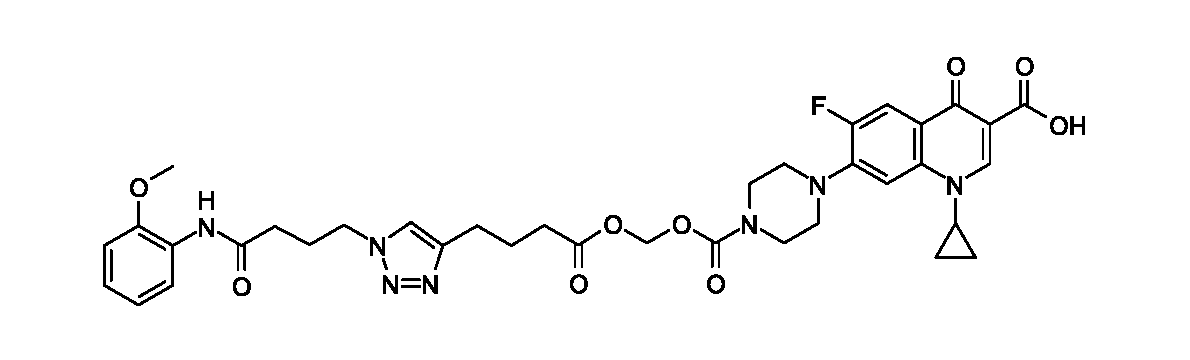
\includegraphics[scale=1]{2MeOA4THCip.eps}
%	\end{center}
%\end{scheme}

\subsection{Methyl 7\hyp{}(4\hyp{}(4\hyp{}(\textit{tert}\hyp{}butoxy)\hyp{}4\hyp{}oxobutyl)piperazin\hyp{}1\hyp{}yl)\hyp{}1\hyp{}cyclopropyl\hyp{}6\hyp{}fluoro\hyp{}4\hyp{}oxo\hyp{}1,4\hyp{}dihydroquinoline\hyp{}3\hyp{}carboxylate \compound{cmpd:tBuOO4CipMe}}

%%LMO\hyp{}2\hyp{}081, LMO\hyp{}2\hyp{}087 (big scale, maybe not pure but done)

\begin{scheme}[H]
	\begin{center}
		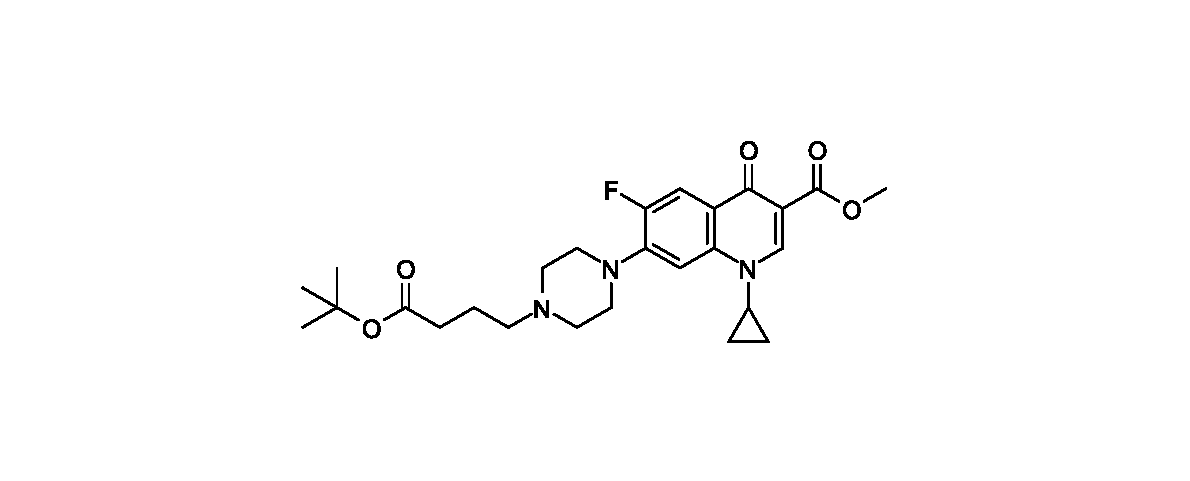
\includegraphics[scale=1]{tBu4CipMe}
	\end{center}
\end{scheme}

Methyl 1\hyp{}cyclopropyl\hyp{}6\hyp{}fluoro\hyp{}4\hyp{}oxo\hyp{}7\hyp{}(piperazin\hyp{}1\hyp{}yl)\hyp{}1,4\hyp{}dihydroquinoline\hyp{}3\hyp{}carboxylate \compound{cmpd:CipMe} (200 mg, 0.579 mmol, 1 eq.), \textit{tert}\hyp{}butyl 4\hyp{}bromobutanoate \compound{cmpd:tBuOO4Br} (103 $\mu$l, 130 mg, 0.581 mmol, 1 eq.), NaI (86.9 mg, 0.580 mmol, 1 eq.), TEA (316 $\mu$l, 229 mg, 2.27 mmol, 4 eq.) and acetonitrile (10 ml) were stirred in a microwave reactor at 100 $^{\circ}$C for 8 h. A second portion of \textit{tert}\hyp{}butyl 4\hyp{}bromobutanoate \compound{cmpd:BocOO4Br} (103 $\mu$l, 130 mg, 0.581 mmol, 1 eq.) was added, and the mixture was stirred in the microwave reactor at 100 $^{\circ}$C for a further 8 h. The mixture was then dry-loaded onto \ce{SiO2} and purified by column chromatography (\ce{SiO2}, 0-4 \% MeOH/\ce{CH2Cl2}). \compound{cmpd:tBuOO4CipMe} was obtained as a white amorphous solid (141 mg, 0.289 mmol, 49.9 \%).
\\[1\baselineskip]
\noindent{\textbf{TLC} \textit{R$_f$} = 0.12 (4 \% MeOH/\ce{CH2Cl2})}
\\[1\baselineskip]
%\noindent{\textbf{mp} \textit{T} / $^{\circ}$C = ?? (??)}
%\\[1\baselineskip]
\noindent{\textbf{IR} (neat) $\nu_{max}$ / cm$^{-1}$ = 
	2961.6 (C-H),
	2830.5 (C-H),
	1732.2 (\textit{t}-Bu ester C=O)
	1717.2 (ciprofloxacin ester C=O),
	1620.6 (quinolone C=O)}
\\[1\baselineskip]
\noindent{\textbf{$^{1}$H NMR} (400 MHz, \ce{CDCl3}) $\delta$ / ppm = 
	8.39 (s, 1 H, \textit{ortho} to C(=O)OCH$_3$), 
	7.82 (d, \textit{J} = 13.3 Hz, 1 H, \textit{ortho} to F), 
	7.17 (d, \textit{J} = 7.2 Hz, 1 H, \textit{meta} to F), 
	3.83 (s, 3 H, C\underline{H}$_3$),
	3.40 (tt, \textit{J} = 7.2, 3.6 Hz, 1 H, NC\underline{H}(CH$_2$)$_2$),
	3.22 (t, \textit{J} = 4.3 Hz, 4 H, CH$_2$N(CH$_2$C\underline{H}$_2$)CH$_2$C\underline{H}$_2$), 
	2.63 (t, \textit{J} = 4.4 Hz, 4 H, CH$_2$N(C\underline{H}$_2$)C\underline{H}$_2$), 
	2.41 (t, \textit{J}=7.3 Hz, 2 H, C\underline{H}$_2$N(CH$_2$)CH$_2$), 
	2.25 (t, \textit{J}=7.4 Hz, 2 H, C\underline{H}$_2$CH$_2$CH$_2$N(CH$_2$)CH$_2$), 
	1.78 (quin, \textit{J}=7.3 Hz, 2 H, C\underline{H}$_2$CH$_2$N(CH$_2$)CH$_2$), 
	1.41 (s, 9 H, C((C\underline{H})$_3$)$_3$), 
	1.24 (m, 2 H, NCH(C\underline{H}H)$_2$), 
	1.09 (m, 2 H, NCH(CH\underline{H})$_2$)}% \todo{should be ranges ideally, go back if time}}
\\[1\baselineskip]
\noindent{\textbf{$^{13}$C NMR} (101 MHz, \ce{CDCl3}) $\delta$ / ppm = 
	172.7 (\underline{C}(=O)CC(=O)OCH$_3$),
	172.6 (\underline{C}(=O)OC(CH$_3$)$_3$), 
	165.9 (\underline{C}(=O)OCH$_3$), 
	153.1 (d, \textit{J} = 249.7 Hz, \textit{ipso} to F), 
	148.1 (\underline{C}=CC(=O)OCH$_3$), 
	144.3 (d, \textit{J} = 10.4 Hz, \textit{ipso} to piperazine), 
	137.7 (\textit{para} to F), 
	122.5 (d, \textit{J} = 6.9 Hz, \textit{para} to piperazine)
	112.6 (d, \textit{J} = 22.5 Hz, \textit{ortho} to C=O and \textit{ortho} to F), 
	109.5 (\underline{C}C(=O)OCH$_3$)
	104.7 (\textit{meta} to C=O and \textit{meta} to F), 
	80.0 (\underline{C}(CH$_3$)$_3$), 
	57.4 (C(=O)CH$_2$CH$_2$\underline{C}H$_2$N), 
	52.7 (C(=O)CH$_2$CH$_2$CH$_2$N(\underline{C}H$_2$)\underline{C}H$_2$), 
	51.7 (\underline{C}H$_3$), 
	49.7 (C(=O)CH$_2$CH$_2$CH$_2$N(CH$_2$\allowbreak \underline{C}H$_2$)CH$_2$CH$_2$), 
	49.7 (C(=O)CH$_2$CH$_2$CH$_2$N(CH$_2$CH$_2$)CH$_2$\underline{C}H$_2$), 
	34.4 (N\underline{C}H(CH$_2$)$_2$), 
	33.2 (C(=O)\underline{C}H$_2$), 
	28.0 (C(\underline{C}H$_3$)$_3$), 
	22.0 (C(=O)CH$_2$\underline{C}H$_2$), 
	7.9 (NCH(\underline{C}H$_2$)$_2$)}
\\[1\baselineskip]
\noindent{\textbf{$^{19}$F NMR} (376.45 MHz, \ce{CDCl3}) $\delta$ / ppm = 
-123.5 (s, ciprofloxacin F)}
\\[1\baselineskip]
\noindent{\textbf{HRMS} (ESI$^+$) \textit{m}/\textit{z} / Da = 488.2562, [M+H]$^+$ found, [\ce{C26H35FN3O5}]$^+$ requires 488.2561}
\\[1\baselineskip]
The compound has not been reported previously.

%\subsection{4\hyp{}(4\hyp{}(1\hyp{}cyclopropyl\hyp{}6\hyp{}fluoro\hyp{}3\hyp{}(methoxycarbonyl)\hyp{}4\hyp{}oxo\hyp{}1,4\hyp{}dihydroquinolin\hyp{}7\hyp{}yl)piperazin\hyp{}1\hyp{}yl)butanoic acid \compound{cmpd:HOO4CipMe}}
%
%%%LMO\hyp{}2\hyp{}079 (using HOO4Br, no reaction)
%
%\begin{scheme}[H]
%	\begin{center}
%		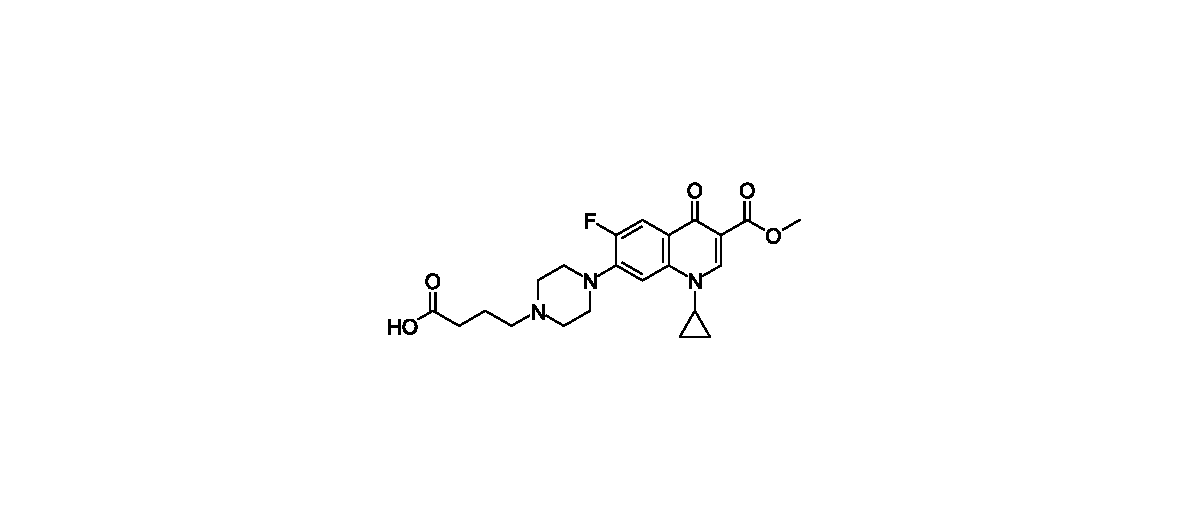
\includegraphics[scale=1]{HOO4CipMe.eps}
%	\end{center}
%\end{scheme}

\subsection{4\hyp{}(4\hyp{}(1\hyp{}Cyclopropyl\hyp{}6\hyp{}fluoro\hyp{}3\hyp{}(methoxycarbonyl)\hyp{}4\hyp{}oxo\hyp{}1,4\hyp{}dihydroquinolin\hyp{}7\hyp{}yl)piperazin\hyp{}1\hyp{}yl)bu\allowbreak tanoic acid trifluoroacetate \compound{cmpd:HOO4CipMeTFA}}

%%LMO\hyp{}2\hyp{}083 (done), LMO\hyp{}2\hyp{}088 (big, purified, is it TFA salt or not??? yes. can see peaks.)

\begin{scheme}[H]
\begin{center}
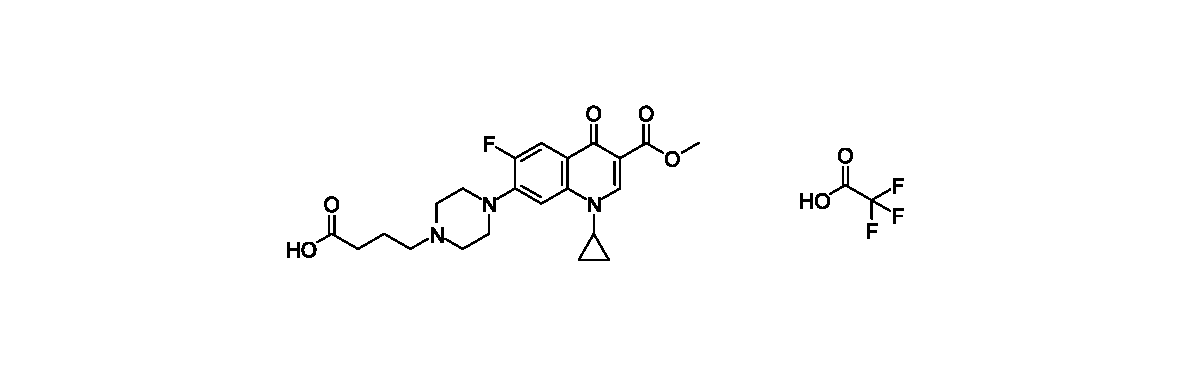
\includegraphics[scale=1]{HOO4CipMeTFA}
\end{center}
\end{scheme}
Methyl 7\hyp{}(4\hyp{}(4\hyp{}(\textit{tert}\hyp{}butoxy)\hyp{}4\hyp{}oxobutyl)piperazin\hyp{}1\hyp{}yl)\hyp{}1\hyp{}cyclopropyl\hyp{}6\hyp{}fluoro\hyp{}4\hyp{}oxo\hyp{}1,4\hyp{}dihydroquinoline\hyp{}3\hyp{}carboxylate \compound{cmpd:tBuOO4CipMe} (20 mg, 41.0 $\mu$mol) and TFA (0.2 ml) were stirred in \ce{CH2Cl2} (1.8 ml) at r.t. for 16 h then evaporated under reduced pressure. \compound{cmpd:HOO4CipMeTFA} was obtained as a white solid (21.4 mg, 39.2 $\mu$mol, 95.6 \%). 
\\[1\baselineskip]
%\noindent{\textbf{TLC} \textit{R$_f$} = ?? (??)}\todo{no rf}
%\\[1\baselineskip]
\noindent{\textbf{mp} \textit{T} / $^{\circ}$C = 225-231 (\ce{CH2Cl2}, decomposes)}
\\[1\baselineskip]
\noindent{\textbf{IR} (neat) $\nu_{max}$ / cm$^{-1}$ = 
	1722.7 (ciprofloxacin ester C=O),
	1699.0 (alkyl carboxylic acid C=O),
	1673.3 (TFA C=O),
	%1626.0 (),
	1614.6 (quinolone C=O)}
\\[1\baselineskip]
\noindent{\textbf{$^{1}$H NMR} (400 MHz, DMSO d$_6$) $\delta$ / ppm = 
	8.47 (s, 1 H, \textit{ortho} to C(=O)OH), 
	7.80 (d, \textit{J} = 13.2 Hz, 1 H, \textit{ortho} to F), 
	7.47 (d, \textit{J} = 7.4 Hz, 1 H, \textit{meta} to F), 
	3.73 (s, 3 H, C\underline{H}$_3$), 
	3.66 (tt, \textit{J} = 7.2, 3.7 Hz, 1 H, NC\underline{H}(CH$_2$)$_2$),
	3.30 - 3.54 (br s, 8 H, CH$_2$N(C\underline{H}$_2$)C\underline{H}$_2$ and CH$_2$N(CH$_2$C\underline{H}$_2$)CH$_2$C\underline{H}$_2$) 
	3.13 - 3.22 (m, 2 H, C\underline{H}$_2$N(CH$_2$)CH$_2$), 
	2.36 (t, \textit{J} = 7.1 Hz, 2 H, C\underline{H}$_2$CH$_2$CH$_2$N(CH$_2$)CH$_2$), 
	1.87 - 1.98 (m, 2 H, C\underline{H}$_2$CH$_2$N(CH$_2$)CH$_2$), 
	1.22 - 1.30 (m, 2 H, NCH(C\underline{H}H)$_2$), 
	1.06 - 1.15 (m, 2 H, NCH(CH\underline{H})$_2$)}
\\[1\baselineskip]
\noindent{\textbf{$^{13}$C NMR} (101 MHz, DMSO d$_6$) $\delta$ / ppm = 
	173.5 (CH$_2$\underline{C}(=O)OH), 
	171.6 (\underline{C}(=O)CC(=O)OCH$_3$), 
	164.9 (\underline{C}(=O)OCH$_3$), 
	158.2 (q, \textit{J} = 31.5 Hz, CF$_3$\underline{C}(=O)OH), 
	152.5 (d, \textit{J} = 247.6 Hz, \textit{ipso} to F), 
	148.5 (\underline{C}=CC(=O)OH), 
	142.3 (d, \textit{J} = 10.7 Hz, \textit{ipso} to piperazine), 
	138.0 (\textit{para} to F), 
	122.6 (d, \textit{J} = 6.4 Hz, \textit{para} to piperazine), 
	117.2 (q, \textit{J} = 299.8 Hz, \underline{C}F$_3$), 
	111.9 (d, \textit{J} = 22.4 Hz, \textit{ortho} to C=O and \textit{ortho} to F), 
	109.1 (\underline{C}C(=O)OCH$_3$), 
	106.9 (\textit{meta} to C=O and \textit{meta} to F), 
	55.1 (C(=O)CH$_2$CH$_2$\underline{C}H$_2$N), 
	51.4 (\underline{C}H$_3$), 
	50.8 (C(=O)CH$_2$CH$_2$CH$_2$N(\underline{C}H$_2$)\underline{C}H$_2$), 
	46.7 (C(=O)CH$_2$CH$_2$CH$_2$N(CH$_2$\underline{C}H$_2$)CH$_2$CH$_2$), 
	46.7 (C(=O)CH$_2$CH$_2$CH$_2$N(CH$_2$CH$_2$)CH$_2$\underline{C}H$_2$), 
	34.9 (N\underline{C}H\allowbreak (CH$_2$)$_2$), 
	30.6 (C(=O)\underline{C}H$_2$), 
	19.1 (C(=O)CH$_2$\underline{C}H$_2$), 
	7.6 (NCH(\underline{C}H$_2$)$_2$)}
\\[1\baselineskip]
\noindent{\textbf{$^{19}$F NMR} (376.45 MHz, DMSO d$_6$) $\delta$ / ppm = 
-73.6 (s, C\underline{F}$_3$), 
-124.6 (s, ciprofloxacin F)}
\\[1\baselineskip]
\noindent{\textbf{HRMS} (ESI$^+$) \textit{m}/\textit{z} / Da = 432.1921, [M+H]$^+$ found, [\ce{C22H27FN3O5}]$^+$ requires 432.1935}
\\[1\baselineskip]
The compound has not been reported previously.

%\subsection{methyl 1\hyp{}cyclopropyl\hyp{}6\hyp{}fluoro\hyp{}7\hyp{}(4\hyp{}(4\hyp{}methoxy\hyp{}4\hyp{}oxobutyl)piperazin\hyp{}1\hyp{}yl)\hyp{}4\hyp{}oxo\hyp{}1,4\hyp{}dihydroquinoline\hyp{}3\hyp{}carboxylate \compound{cmpd:MeOO4CipMe}}
%
%%%LMO\hyp{}2\hyp{}080 (using MeOO4Cl, done, but not useful, need boc)
%
%\begin{scheme}[H]
%	\begin{center}
%		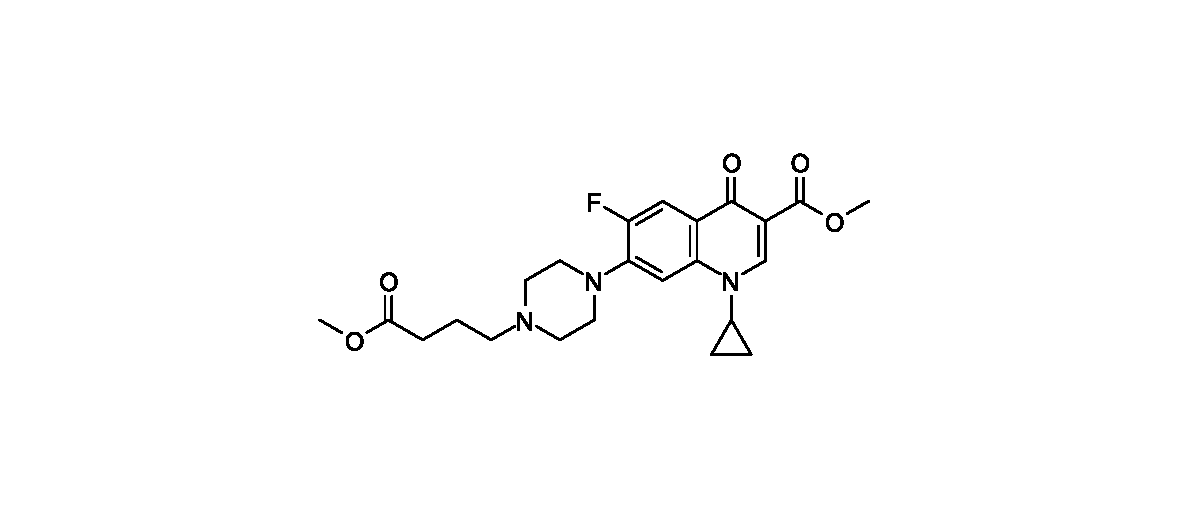
\includegraphics[scale=1]{MeOO4CipMe}
%	\end{center}
%\end{scheme}
%
%Can't find NMR, don't bother including?
%
%\subsection{methyl (\textit{S})\hyp{}1\hyp{}cyclopropyl\hyp{}6\hyp{}fluoro\hyp{}4\hyp{}oxo\hyp{}7\hyp{}(4\hyp{}(4\hyp{}oxo\hyp{}4\hyp{}((2\hyp{}oxotetrahydrofuran\hyp{}3\hyp{}yl)amino)butyl)piperazin\hyp{}1\hyp{}yl)\hyp{}1,4\hyp{}dihydroquinoline\hyp{}3\hyp{}carboxylate \compound{cmpd:HL4CipMe}}
%
%%%LMO\hyp{}2\hyp{}089 (done as a test, worked but not purified)
%
%\begin{scheme}[H]
%	\begin{center}
%		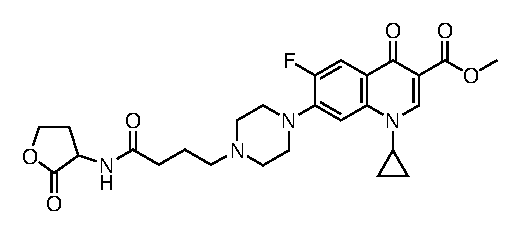
\includegraphics[scale=1]{HL4CipMe}
%	\end{center}
%\end{scheme}

\subsection{(1\textit{R},2\textit{R})\hyp{}2\hyp{}(((\textit{S})\hyp{}1\hyp{}Phenylethyl)amino)\allowbreak cyclopentan\hyp{}1\hyp{}ol \compound{cmpd:HOcy5NHMeBn_RRS} and (1\textit{S},2\textit{S})\hyp{}2\hyp{}(((\allowbreak \textit{S})\hyp{}1\hyp{}phenylethyl)am\allowbreak ino)cyclopentan\hyp{}1\hyp{}ol \compound{cmpd:HOcy5NHMeBn_SSS}}

%%LMO\hyp{}2\hyp{}044, LMO\hyp{}2\hyp{}053 (big)

\begin{scheme}[H]
	\begin{center}
		\schemeref[HOcy5NHMeBn_RRS]{cmpd:HOcy5NHMeBn_RRS}
		\schemeref[HOcy5NHMeBn_SSS]{cmpd:HOcy5NHMeBn_SSS}
		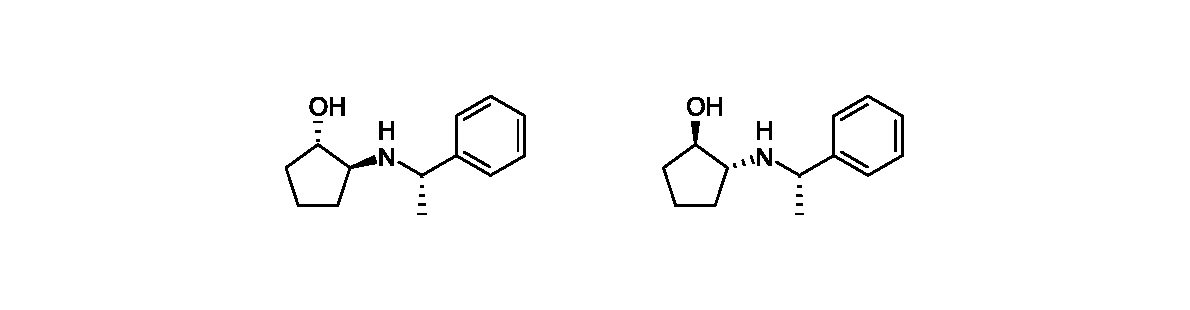
\includegraphics[scale=1]{HOcy5NHMeBn_both.eps}
	\end{center}
\end{scheme}
(\textit{S})-1-Phenylethan-1-amine \compound{cmpd:NH2MeBn} (7.85 ml, 7.38 g, 60.9 mmol, 1 eq.) was dissolved in \ce{CH2Cl2} (50 ml) and stirred rapidly at 0 $^\circ$C. A solution of \ce{AlMe3} (31 ml, 2.0 M in heptane, 60.9 mmol) was added dropwise and the mixture was stirred at 0 $^\circ$C for 1 h. A solution of cyclohexene oxide \compound{cmpd:Ocy} (5.71 ml, 5.50 g, 65.4 mmol, 1.1 eq.) in \ce{CH2Cl2} (50 ml) was then added dropwise, and the mixture was stirred at 0 $^\circ$C for a further 3 h, followed by 48 h at r.t.. The mixture was cooled  to 0 $^\circ$C and NaF (11 g, 262 mmol, 4.3 eq.) was added portionwise, followed by water (7.00 ml, 7.00 g, 389 mmol, 6.4 eq.) and \ce{CH2Cl2} (50 ml). The suspension was allowed to warm to r.t. and stirred for 1 h, then filtered through Celite and washed with \ce{CH2Cl2} (500 ml). The filtrate was dried with \ce{K2CO3}, concentrated under reduced pressure and purified by column chromatography (\ce{SiO2}, 20:5:1 hexane:EtOAc:TEA). \compound{cmpd:HOcy5NHMeBn_RRS} was obtained as a pale yellow oil (4.08 g, 19.9 mmol, 32.6 \%). \compound{cmpd:HOcy5NHMeBn_SSS} was obtained as pale yellow crystals (4.48 g, 21.8 mmol, 35.8 \%).

\subsubsection*{(1\textit{R},2\textit{R})\hyp{}2\hyp{}(((\textit{S})\hyp{}1\hyp{}Phenylethyl)amino)cyclopentan\hyp{}1\hyp{}ol \compound{cmpd:HOcy5NHMeBn_RRS}}
\noindent{\textbf{TLC} \textit{R$_f$} = 0.25 (15:5:1 hexane:EtOAc:TEA)}
\\[1\baselineskip]
\noindent{\textbf{IR} (neat) $\nu_{max}$ / cm$^{-1}$ = 
	3300.0 (br, O-H),
	2959.7 (C-H),
	2870.1 (C-H)}
\\[1\baselineskip]
\noindent{\textbf{$^{1}$H NMR} (400 MHz, \ce{CDCl3}) $\delta$ / ppm = 
	7.28 - 7.38 (m, 4 H, \textit{ortho} and \textit{meta} to CHCH$_3$), 
	7.21 - 7.28 (m, 1 H, \textit{para} to CHCH$_3$), 
	3.83 (q, \textit{J} = 6.6 Hz, 1 H, C\underline{H}CH$_3$), 
	3.78 (q, \textit{J} = 7.0 Hz, 1 H, C\underline{H}OH), 
	2.62 (dt, \textit{J} = 8.2, 7.2 Hz, 1 H, C\underline{H}NH), 
	1.97 (quin, \textit{J} = 6.7 Hz, 1 H, C\underline{H}$_2$CHNH), 
	1.90 (quin, \textit{J} = 6.9 Hz, 1 H, C\underline{H}$_2$CHOH), 
	1.56 - 1.68 (m, C\underline{H}$_2$CH$_2$CHOH), 
	1.43 (dq, \textit{J} = 12.5, 8.0 Hz, 1 H, C\underline{H}$_2$CHOH), 
	1.37 (d, \textit{J} = 6.6 Hz, 3 H, C\underline{H}$_3$), 
	1.25 - 1.36 (m, 1 H, C\underline{H}$_2$CHNH)}
\\[1\baselineskip]
\noindent{\textbf{$^{13}$C NMR} (101 MHz, \ce{CDCl3}) $\delta$ / ppm = 
	144.75 (\textit{ipso} to CHCH$_3$), 
	128.26 (\textit{meta} to CHCH$_3$), 
	126.72 (\textit{para} to CHCH$_3$), 
	126.30 (\textit{ortho} to CHCH$_3$), 
	77.65 (\underline{C}HOH), 
	63.38 (\underline{C}HNH), 
	56.20 (\underline{C}HCH$_3$), 
	31.74 (\underline{C}H$_2$CHOH), 
	29.22 (\underline{C}H$_2$CHNH), 
	24.58 (\underline{C}H$_3$), 
	19.57 (\underline{C}H$_2$CH$_2$CHOH)}
\\[1\baselineskip]
\noindent{\textbf{HRMS} (ESI$^+$) \textit{m}/\textit{z} / Da = 206.1554, [M+H]$^+$ found, [\ce{C13H20NO}]$^+$ requires 206.1545}
\\[1\baselineskip]
\noindent{[\bm{$\alpha$}]$_D^{20}$ / $^{\circ}$10$^{-1}$cm$^2$g$^{-1}$ = -92.8 (\textit{c} / g(100 ml)$^{-1}$ = 1.19, MeOH)}

\subsubsection*{(1\textit{S},2\textit{S})\hyp{}2\hyp{}(((\textit{S})\hyp{}1\hyp{}Phenylethyl)amino)cyclopentan\hyp{}1\hyp{}ol \compound{cmpd:HOcy5NHMeBn_SSS}}
\noindent{\textbf{TLC} \textit{R$_f$} = 0.36 (15:5:1 hexane:EtOAc:TEA)}
\\[1\baselineskip]
\noindent{\textbf{mp} \textit{T} / $^{\circ}$C = 66-71.5 (hexane, EtOAc, TEA)}
\\[1\baselineskip]
\noindent{\textbf{IR} (neat) $\nu_{max}$ / cm$^{-1}$ = 
	3150.0 (br, O-H),
	2950.9 (C-H),
	2868.2 (C-H)}
\\[1\baselineskip]
\noindent{\textbf{$^{1}$H NMR} (400 MHz, \ce{CDCl3}) $\delta$ / ppm =
	7.28 - 7.34 (m, 4 H, \textit{ortho} and \textit{meta} to CHCH$_3$), 
	7.20 - 7.26 (m, 1 H, \textit{para} to CHCH$_3$), 
	3.86 (q, \textit{J} = 6.6 Hz, 1 H, C\underline{H}CH$_3$), 
	3.85 (q, \textit{J} = 6.6 Hz, 1 H, C\underline{H}OH), 
	2.83 (td, \textit{J} = 7.6, 5.7 Hz, 1 H, C\underline{H}NH), 
	1.85 - 1.97 (m, 1 H, C\underline{H}HCHOH), 
	1.77 (dtd, \textit{J} = 12.9, 7.9, 7.9, 4.9 Hz, 1 H, C\underline{H}HCHNH), 
	1.55 - 1.68 (m, 2 H, C\underline{H}$_2$CH$_2$CHOH), 
	1.47 - 1.55 (m, 1 H, CH\underline{H}CHOH), 
	1.36 (d, \textit{J} = 6.6 Hz, 3 H, C\underline{H}$_3$), 
	1.12 (dq, \textit{J} = 12.7, 8.1 Hz, 1 H, CH\underline{H}CHNH)}
\\[1\baselineskip]
\noindent{\textbf{$^{13}$C NMR} (101 MHz, \ce{CDCl3}) $\delta$ / ppm = 
	145.61 (\textit{ipso} to CHCH$_3$), 
	128.08 (\textit{meta} to CHCH$_3$), 
	126.61 (\textit{para} to CHCH$_3$), 
	126.33 (\textit{ortho} to CHCH$_3$), 
	77.43 (\underline{C}HOH), 
	64.45 (\underline{C}HNH), 
	56.62 (\underline{C}HCH$_3$), 
	32.01 (\underline{C}H$_2$CHOH), 
	30.56 (\underline{C}H$_2$CHNH), 
	23.30 (\underline{C}H$_3$), 
	20.06 (\underline{C}H$_2$CH$_2$CHOH)}
\\[1\baselineskip]
\noindent{\textbf{HRMS} (ESI$^+$) \textit{m}/\textit{z} / Da = 206.1553, [M+H]$^+$ found, [\ce{C13H20NO}]$^+$ requires 206.1545}
\\[1\baselineskip]
\noindent{[\bm{$\alpha$}]$_D^{20}$ / $^{\circ}$10$^{-1}$cm$^2$g$^{-1}$ = -23.9 (\textit{c} / g(100 ml)$^{-1}$ = 0.96 , MeOH)}
\\[1\baselineskip]
The compounds have been synthesised previously\cite{Aube1992,Overman1985}, but NMR data were not published. The enantiomers of both compounds have also been synthesised previously, and the $^{1}$H NMR data for these are consistent with the the above data\cite{Overman1985a}.

%\subsection{(1\textit{S},2\textit{S})\hyp{}2\hyp{}(((\textit{S})\hyp{}1\hyp{}phenylethyl)amino)cyclopentan\hyp{}1\hyp{}ol hydrochloride \compound{cmpd:HOcy5NHMeBn(SSS)HCl}}
%
%\begin{scheme}[H]
%	\begin{center}
%		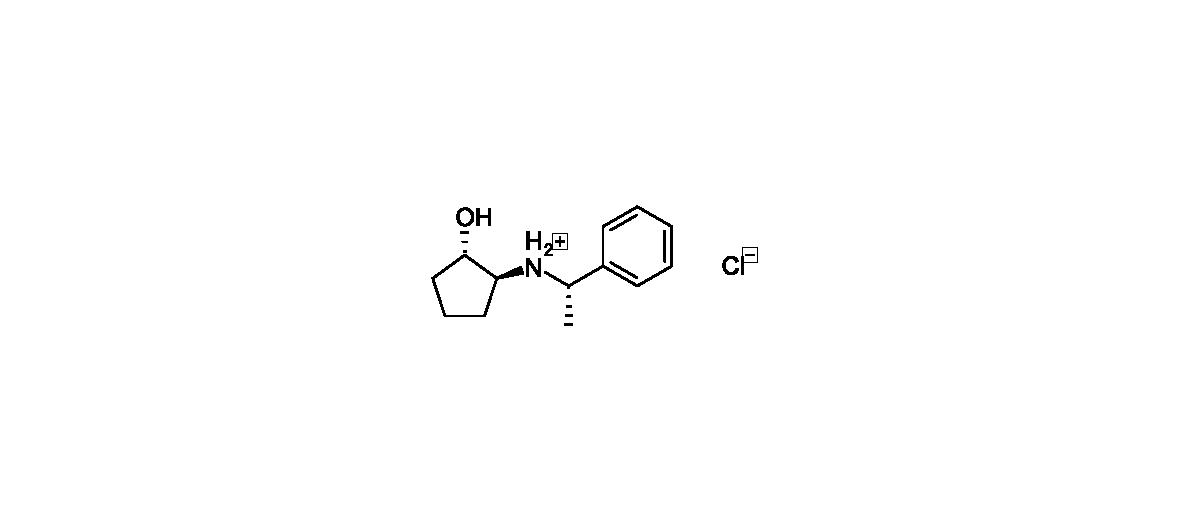
\includegraphics[scale=1]{HOcy5NHMeBn(SSS)HCl.eps}
%	\end{center}
%\end{scheme}
%
%\subsection{(1\textit{R},2\textit{R})\hyp{}2\hyp{}(((\textit{S})\hyp{}1\hyp{}phenylethyl)amino)cyclopentan\hyp{}1\hyp{}ol hydrochloride \compound{cmpd:HOcy5NHMeBn(RRS)HCl}} 
%
%%%LMO\hyp{}2\hyp{}046, LMO\hyp{}2\hyp{}052 
%
%%%only have 1H NMR so not documenting
%
%\begin{scheme}[H]
%	\begin{center}
%		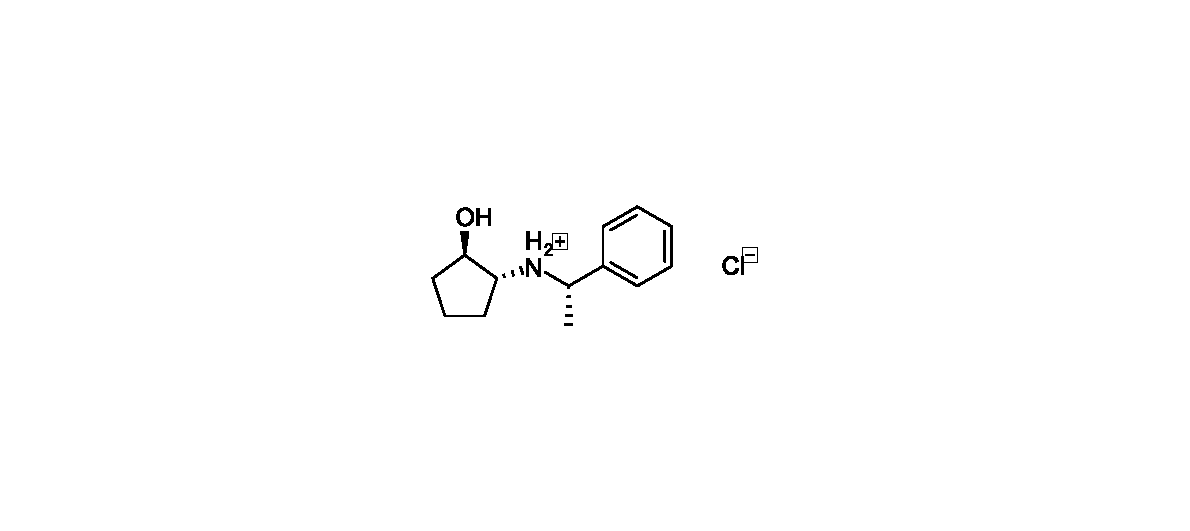
\includegraphics[scale=1]{HOcy5NHMeBn(RRS)HCl.eps}
%	\end{center}
%\end{scheme}

\subsection{(1\textit{R},2\textit{R})\hyp{}2\hyp{}Aminocyclopentan\hyp{}1\hyp{}ol \compound{cmpd:HOcy5NH2_RR}}

%%LMO\hyp{}2\hyp{}050 (just to salt, Pd/C, NH4HCO2), LMO\hyp{}2\hyp{}061 (worked)

\begin{scheme}[H]
	\begin{center}
		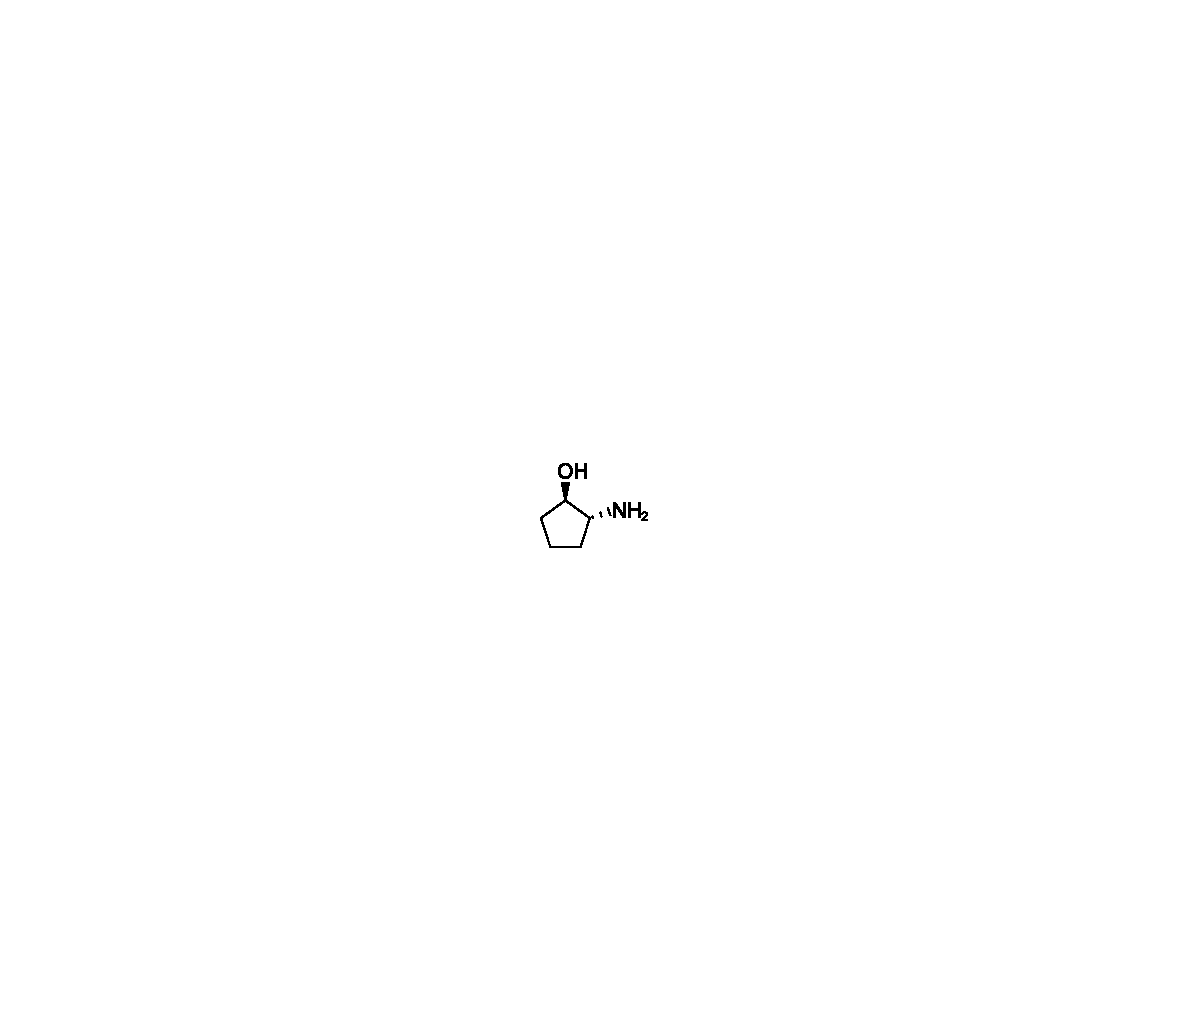
\includegraphics[scale=1]{HOcy5NH2(RR).eps}
	\end{center}
\end{scheme}

(1\textit{R},2\textit{R})\hyp{}2\hyp{}(((\textit{S})\hyp{}1\hyp{}Phenylethyl)amino)cyclopentan\hyp{}1\hyp{}ol \compound{cmpd:HOcy5NHMeBn_RRS} (3.90 g, 19.0 mmol, 1 eq.), \ce{Pd(OH)2} (20 wt. \% on C, moistened with 50 wt. \% water, 1 g, 0.712 mmol, 0.04 eq.) and MeOH (50 ml) were stirred in a Paar hydrogenator at r.t. and 3 atm for 2 days. The mixture was then filtered through Celite and evaporated under reduced pressure. \compound{cmpd:HOcy5NH2_RR} was obtained as a yellow oil (1.92 g, 19.0 mmol, 100 \%).
\\[1\baselineskip]
\noindent{\textbf{TLC} \textit{R$_f$} = 0.10 (10 \% MeOH/\ce{CH2Cl2})}
\\[1\baselineskip]
\noindent{\textbf{IR} (neat) $\nu_{max}$ / cm$^{-1}$ = 
	3300.0 (br, O-H),
	2958.3 (C-H),
	2871.5 (C-H)}
\\[1\baselineskip]
\noindent{\textbf{$^{1}$H NMR} (400 MHz, MeOD) $\delta$ / ppm = 
	3.77 (ddd, J=6.6, 6.2, 5.6, 1 H, C\underline{H}OH), 
	3.00 (td, J=7.3, 5.6 Hz, 1 H, C\underline{H}NH$_2$), 
	2.00 (dtd, J=13.0, 7.7, 7.7, 5.6 Hz, 1 H, C\underline{H}HCHNH$_2$), 
	1.97 (ddt, J=13.0, 8.7, 6.6, 6.6 Hz, 1 H, C\underline{H}HCHOH), 
	1.63 - 1.77 (m, 2 H, C\underline{H}$_2$CH$_2$CHOH), 
	1.53 (ddt, J=13.0, 9.5, 6.2, 6.2 Hz, 1 H, CH\underline{H}CHOH), 
	1.37 (ddt, J=13.0, 8.3, 7.8, 7.8 Hz, 1 H, CH\underline{H}CHNH$_2$)}
\\[1\baselineskip]
\noindent{\textbf{$^{13}$C NMR} (101 MHz, MeOD) $\delta$ / ppm = 
	80.7 (\underline{C}HOH), 
	60.8 (\underline{C}HNH$_2$), 
	33.2 (\underline{C}H$_2$CHOH), 
	32.1 (\underline{C}H$_2$CHNH$_2$), 
	21.2 (\underline{C}H$_2$CH$_2$CHOH)}
\\[1\baselineskip]
\noindent{\textbf{HRMS} (ESI$^+$) \textit{m}/\textit{z} / Da = 102.0917, [M+H]$^+$ found, [\ce{C5H12NO}]$^+$ requires 102.0913}
\\[1\baselineskip]	
\noindent{[\bm{$\alpha$}]$_D^{20}$ / $^{\circ}$10$^{-1}$cm$^2$g$^{-1}$ = -30.9 (\textit{c} / g(100 ml)$^{-1}$ = 1.5 , EtOH)}
\\[1\baselineskip]
The data are consistent with the literature\cite{Schiffers2006,Overman1985}.
	
%(1S,2S)-trans-2-Amino-1-cyclopentanol (37) According to GP-3, the title compound was
%prepared by hydrogenation of (1S,2S)-38 (857 mg, 4.48 mmol): 440 mg (97%); mp 78.5 °C; [α] 25
%D =
%+36.3 (c = 1.13, MeOH); 1
%H-NMR (400 MHz, CDCl3) δ 1.26-1.37 (1 H, m), 1.48-1.58 (1 H, m),
%1.59-1.77 (2 H, m), 1.92-2.04 (2 H, m), 3.01 (1 H, dd, J = 7.7, 14.3 Hz), 3.22 (3 H, br s), 3.73 (1 H, q,
%J = 6.9 Hz); 1 3C-NMR (100 MHz, CDCl3) δ 19.7, 32.0, 59.7, 79.3; IR (KBr) ν = 3540, 3476, 3449,
%3424, 3362, 3301, 2947, 2931, 1450, 1427, 1085 cm−1
%; MS (EI, DIP) m/z 102 (7), 101 (88), 100 (32),
%84 (30), 83 (13), 82 (33), 72 (19), 68 (15), 57 (60), 56 (100), 55 (25); HRMS Calcd for C5H1 1NO:
%101.0841. Found: 101.0840.

\subsection{(1\textit{S},2\textit{S})\hyp{}2\hyp{}Aminocyclopentan\hyp{}1\hyp{}ol \compound{cmpd:HOcy5NH2_SS}}

%%LMO\hyp{}2\hyp{}047 (no? from salt), LMO\hyp{}2\hyp{}048 (no? from free amine), LMO\hyp{}2\hyp{}049 (just to salt, Pd/C, NH4HCO2), LMO\hyp{}2\hyp{}051 (just to salt, Pd/C, NH4HCO2, acetic acid, mess), LMO\hyp{}2\hyp{}054 (just to salt, Pd/C, NH4HCO2), LMO\hyp{}2\hyp{}055 (Pd(OH)2, H2, maybe?), LMO\hyp{}2\hyp{}056 (salt, Pd(OH)2, H2, maybe?), LMO\hyp{}2\hyp{}057  (free amine, Pd(OH)2, H2, 5 atm, YES), LMO\hyp{}2\hyp{}059 (big,yes)

\begin{scheme}[H]
	\begin{center}
		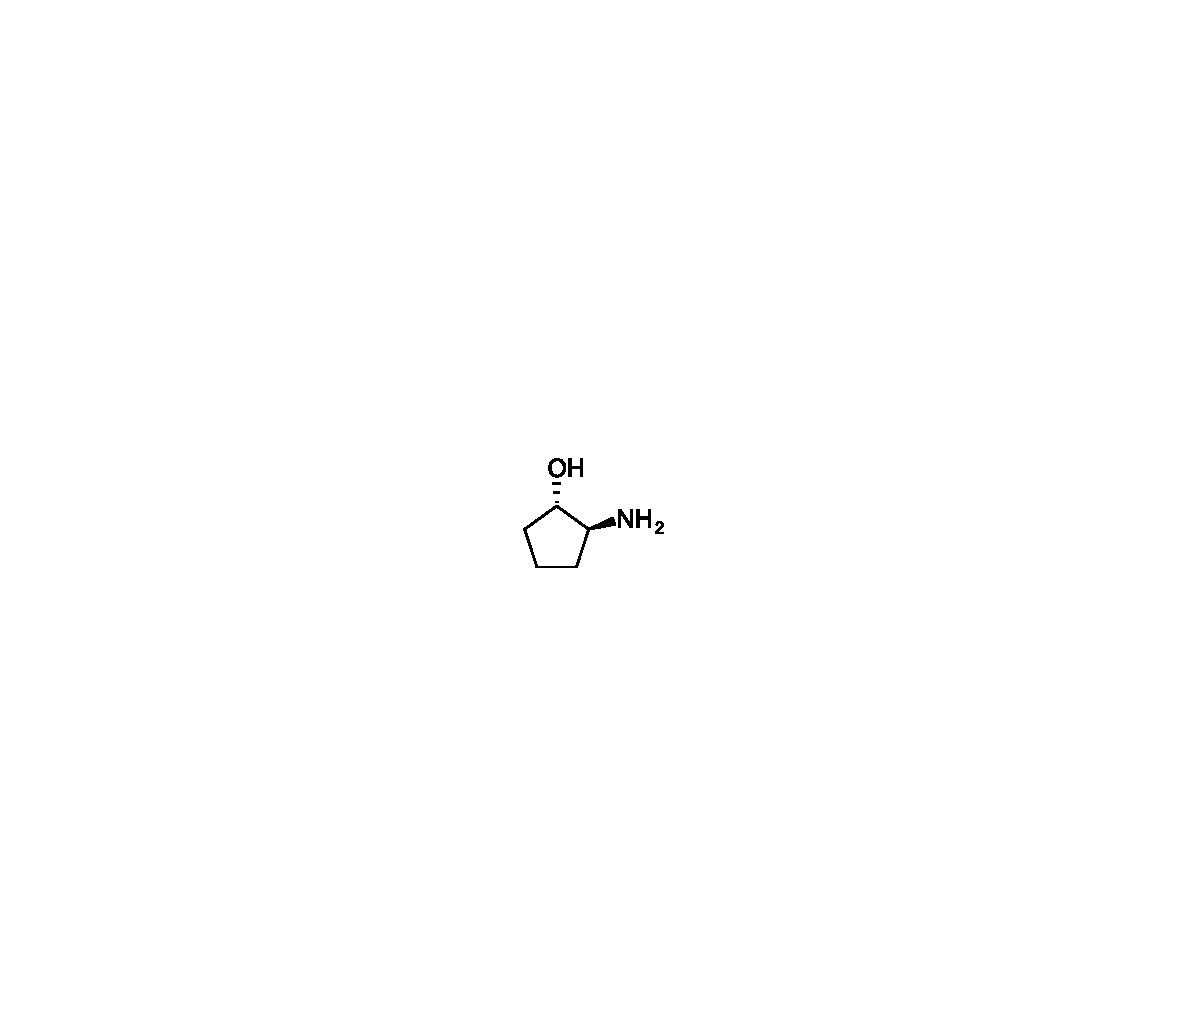
\includegraphics[scale=1]{HOcy5NH2(SS).eps}
	\end{center}
\end{scheme}

(1\textit{S},2\textit{S})\hyp{}2\hyp{}(((\textit{S})\hyp{}1\hyp{}Phenylethyl)amino)cyclopentan\hyp{}1\hyp{}ol \compound{cmpd:HOcy5NHMeBn_SSS} (3.00 g, 14.6 mmol, 1 eq.), \ce{Pd(OH)2} (20 wt. \% on C, moistened with 50 wt. \% water, 0.5 g, 0.356 mmol, 0.025 eq.) and MeOH (50 ml) were stirred in a Paar hydrogenator at r.t. and 2.5 atm for 2 days. The mixture was then filtered through Celite and evaporated under reduced pressure. \compound{cmpd:HOcy5NH2_SS} was obtained as a yellow oil (1.48 g, 14.6 mmol, 100 \%).
\\[1\baselineskip]
\noindent{\textbf{TLC} \textit{R$_f$} = 0.10 (10 \% MeOH/\ce{CH2Cl2})}
\\[1\baselineskip]
\noindent{\textbf{IR} (neat) $\nu_{max}$ / cm$^{-1}$ = 
	3300.0 (O-H),
	2969.2 (C-H),
	2872.7 (C-H)}
\\[1\baselineskip]
\noindent{\textbf{$^{1}$H NMR} (400 MHz, MeOD) $\delta$ / ppm =
	3.77 (ddd, J=6.6, 6.2, 5.6, 1 H, C\underline{H}OH), 
	3.00 (td, \textit{J} = 7.4, 5.6 Hz, 1 H, C\underline{H}NH$_2$), 
	2.00 (dtd, \textit{J} = 13.0, 7.7, 7.7, 5.6 Hz, 1 H, C\underline{H}HCHNH$_2$), 
	1.97 (ddt, \textit{J} = 13.0, 8.7, 6.4, 6.4 Hz, 1 H, C\underline{H}HCHOH), 
	1.64 - 1.77 (m, 2 H, C\underline{H}$_2$CH$_2$CHOH), 
	1.53 (ddt, \textit{J} = 13.0, 9.5, 6.2, 6.2 Hz, 1 H, CH\underline{H}CHOH), 
	1.37 (ddt, \textit{J} = 12.8, 8.5, 7.7, 7.7 Hz, 1 H, CH\underline{H}CHNH$_2$)}
\\[1\baselineskip]
\noindent{\textbf{$^{13}$C NMR} (101 MHz, MeOD) $\delta$ / ppm = 
	80.6 (\underline{C}HOH), 
	60.7 (\underline{C}HNH$_2$), 
	33.2 (\underline{C}H$_2$CHOH), 
	32.2 (\underline{C}H$_2$CHNH$_2$), 
	21.2 (\underline{C}H$_2$CH$_2$CHOH)}
\\[1\baselineskip]
\noindent{\textbf{HRMS} (ESI$^+$) \textit{m}/\textit{z} / Da = 102.0915, [M+H]$^+$ found, [\ce{C5H12NO}]$^+$ requires 102.0913}
\\[1\baselineskip]
\noindent{[\bm{$\alpha$}]$_D^{20}$ / $^{\circ}$10$^{-1}$cm$^2$g$^{-1}$ = 33.4 (\textit{c} / g(100 ml)$^{-1}$ = 0.5, EtOH)}
\\[1\baselineskip]
The data are consistent with the literature\cite{Schiffers2006,Overman1985}.

\subsection{(1\textit{S},2\textit{S})\hyp{}2\hyp{}((\textit{tert}\hyp{}Butyldimethylsilyl)oxy)cyclopentan\hyp{}1\hyp{}amine \compound{cmpd:TBSOcy5NH2_SS}}

%%Find table in presentation for details
%%LMO\hyp{}2\hyp{}060 (maybe), LMO\hyp{}2\hyp{}062 (no), LMO\hyp{}2\hyp{}063 (lost), LMO\hyp{}2\hyp{}064 (no?), LMO\hyp{}2\hyp{}065 (no reaction), LMO\hyp{}2\hyp{}066 (no prod?), LMO\hyp{}2\hyp{}067 (makes HCl salt of SM), LMO\hyp{}2\hyp{}068 (yes? not sure if amine or salt), LMO\hyp{}2\hyp{}070 (yes but column fail), LMO\hyp{}2\hyp{}071 (yes)
%%no evidence of it being salt in NMR (070) 

\begin{scheme}[H]
	\begin{center}
		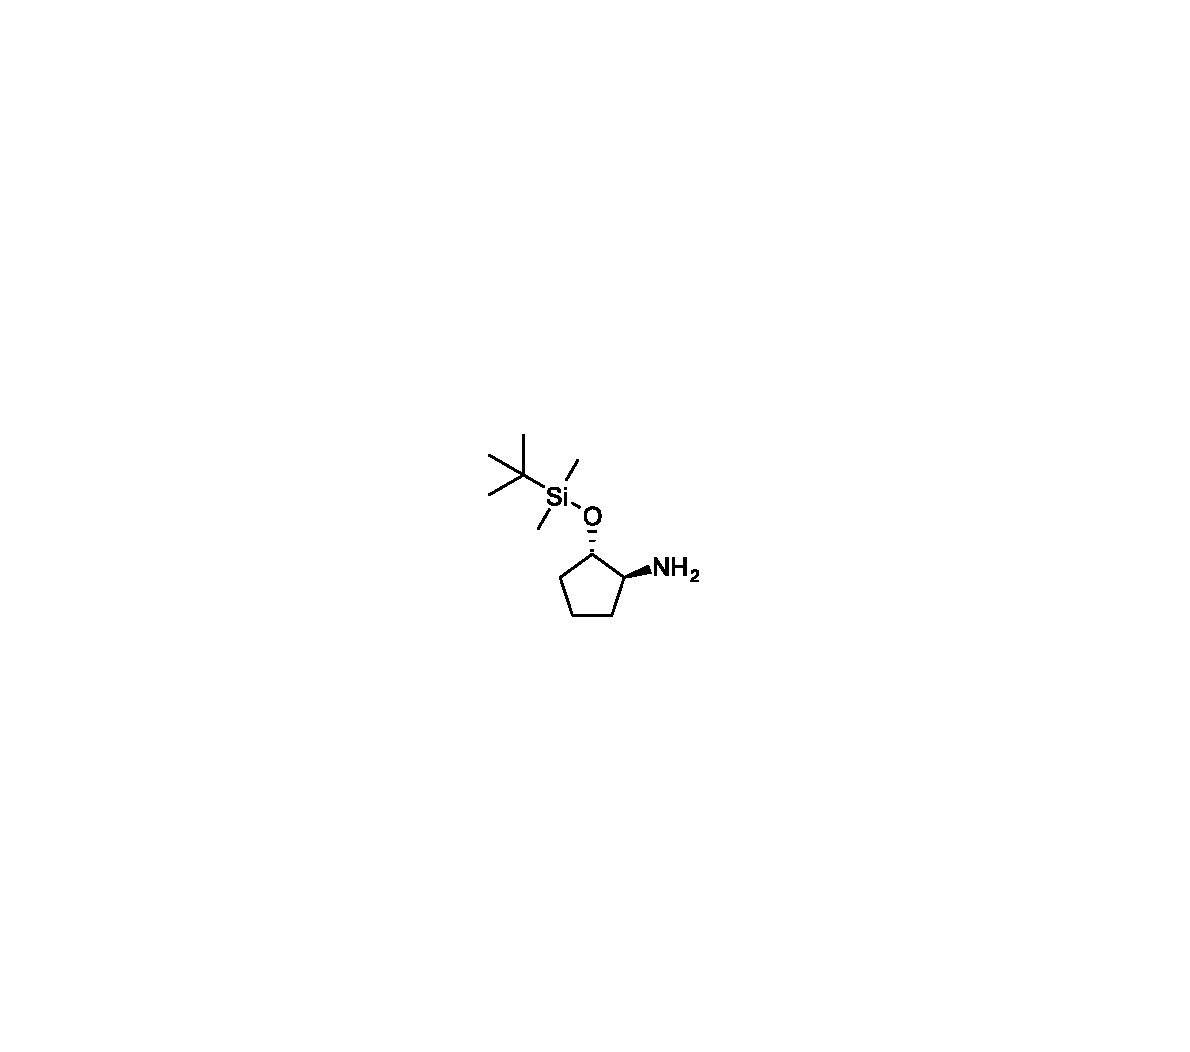
\includegraphics[scale=1]{TBSOcy5NH2(SS).eps}
	\end{center}
\end{scheme}

(1\textit{S},2\textit{S})\hyp{}2\hyp{}Aminocyclopentan\hyp{}1\hyp{}ol \compound{cmpd:HOcy5NH2_SS} (0.480 g, 4.75 mmol) was stirred in dry \ce{CH2Cl2} (20 ml) under \ce{N2} at 0 $^\circ$C. TEA (3.14 ml, 2.28 g, 22.5 mmol, 5 eq.) was added dropwise, followed by TBSOTf (3 ml, 3.45 g, 13.1 mmol, 3 eq.) dropwise. The reaction was allowed to reach r.t. and stirred for 1 h. The reaction was quenched with \ce{NH4Cl}, diluted with \ce{CH2Cl2} (20 ml) and washed with water (20 ml). The organic phase was dried with \ce{Na2\textit{S}O4}, concentrated under reduced pressure and purified by column chromatography (\ce{SiO2}, 4 \% MeOH/\ce{CH2Cl2}). \compound{cmpd:TBSOcy5NH2_SS} was obtained as a yellow oil (1.00 g, 4.64 mmol, 97.7 \%).
\\[1\baselineskip]
\noindent{\textbf{TLC} \textit{R$_f$} = 0.23 (10 \% MeOH/\ce{CH2Cl2})}
\\[1\baselineskip]
\noindent{\textbf{IR} (neat) $\nu_{max}$ / cm$^{-1}$ = 
	2953.6 (C-H),
	2931.1 (C-H),
	2888.4 (C-H),
	2858.8 (C-H),
	1625.2 (N-H bend)} 
\\[1\baselineskip]
\noindent{\textbf{$^{1}$H NMR} (400 MHz, \ce{CDCl3}) $\delta$ / ppm =
	4.13 (q, \textit{J} = 5.8 Hz, 1 H, C\underline{H}OSi), 
	3.31 (td, \textit{J} = 7.1, 5.2 Hz, 1 H, C\underline{H}NH$_2$), 
	2.09 - 2.19 (m, 1 H, C\underline{H}HCHNH$_2$), 
	1.97 (ddq, \textit{J} = 8.8, 7.0, 6.0, 6.0, 6.0 Hz, 1 H, C\underline{H}HCHOSi), 
	1.74 - 1.86 (m, 2 H, C\underline{H}$_2$CH$_2$CHOSi), 
	1.64 - 1.74 (m, 1 H, CH\underline{H}CHOSi), 
	1.58 (ddt, \textit{J} = 13.2, 9.1, 6.0, 6.0 Hz, 1 H, CH\underline{H}CHNH$_2$), 
	0.88 (s, 9 H, C(C\underline{H}$_3$)$_3$), 
	0.09 (s, 3 H, SiC\underline{H}$_3$), 
	0.07 (s, 3 H, SiC\underline{H}$_3$)}
\\[1\baselineskip]
\noindent{\textbf{$^{13}$C NMR} (101 MHz, \ce{CDCl3}) $\delta$ / ppm = 
	76.3 (\underline{C}HOSi), 
	59.7 (\underline{C}HNH), 
	32.2 (\underline{C}H$_2$CHOSi), 
	26.8 (\underline{C}H$_2$CHNH$_2$), 
	25.6 (C(\underline{C}H$_3$)$_3$), 
	19.7 (\underline{C}H$_2$CH$_2$CHOSi), 
	17.7 (\underline{C}(CH$_3$)$_3$), 
	-4.8 (Si\underline{C}H$_3$), 
	-5.2 (Si\underline{C}H$_3$)}
\\[1\baselineskip]
\noindent{\textbf{HRMS} (ESI$^+$) \textit{m}/\textit{z} / Da = 216.1785, [M+H]$^+$ found, [\ce{C11H26NOSi}]$^+$ requires 216.1784}
%\\[1\baselineskip]
%\noindent{[\bm{$\alpha$}]$_D^{20}$ / $^{\circ}$10$^{-1}$cm$^2$g$^{-1}$ = ?? (\textit{c} / g(100 ml)$^{-1}$ = ?? , MeOH)}\todo{get??}
The compound has not been reported previously.


%\subsection{4\hyp{}bromo\hyp{}N\hyp{}((1\textit{R},2\textit{R})\hyp{}2\hyp{}hydroxycyclopentyl)butanamide \compound{cmpd:HOcy5NH4Br(RR)}}
%
%%%LMO\hyp{}2\hyp{}058 (messy)
%
%\begin{scheme}[H]
%	\begin{center}
%		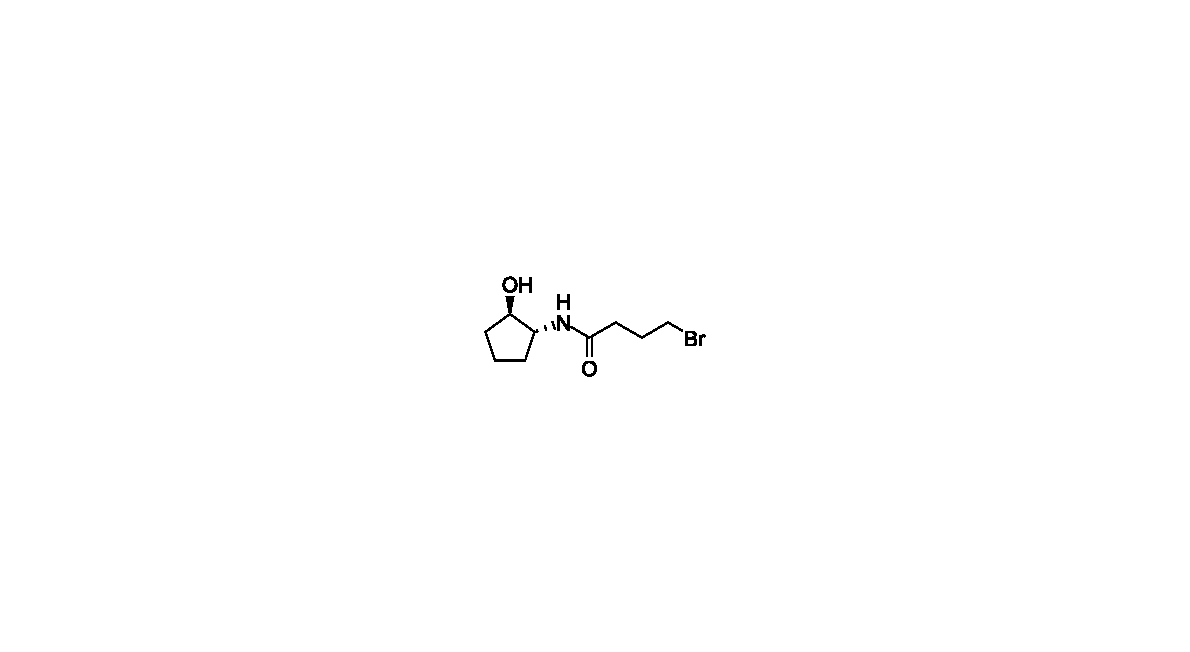
\includegraphics[scale=1]{HOcy5NH4Br(RR).eps}
%	\end{center}
%\end{scheme}

%\subsection{4\hyp{}bromo\hyp{}N\hyp{}((1\textit{R},2\textit{R})\hyp{}2\hyp{}((\textit{tert}\hyp{}butyldimethylsilyl)oxy)cyclopentyl)butanamide \compound{cmpd:TBSOcy5NH4Br(RR)}}
%
%%%LMO\hyp{}2\hyp{}069 (mostly hydrolysis), LMO\hyp{}2\hyp{}072 (??? didn't write anything), LMO\hyp{}2\hyp{}073 (failed on purification, concentration issues)
%
%\begin{scheme}[H]
%	\begin{center}
%		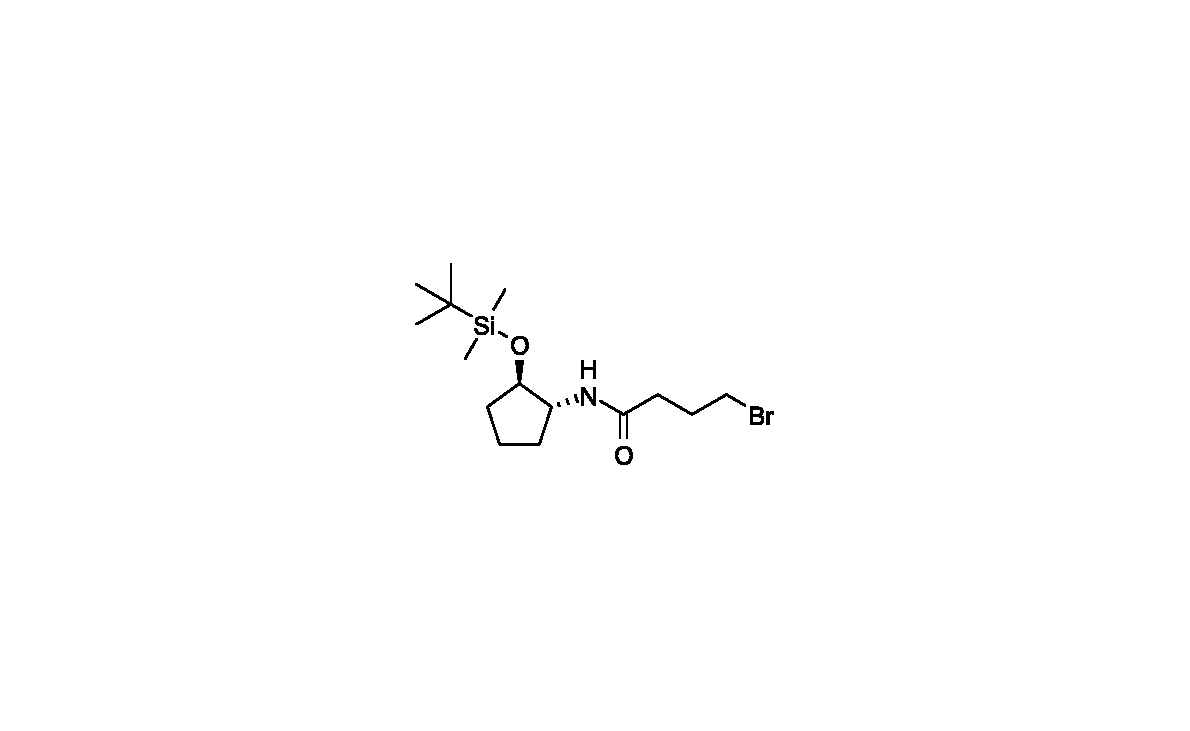
\includegraphics[scale=1]{TBSOcy5NH4Br(RR).eps}
%	\end{center}
%\end{scheme}

\subsection{4\hyp{}Chloro\hyp{}\textit{N}\hyp{}((1\textit{R},2\textit{R})\hyp{}2\hyp{}hydroxycyclopentyl)butanamide \compound{cmpd:HOcy5NH4Cl_RR}}

%%LMO\hyp{}2\hyp{}092 (Schotten Bauman, doesn't work), LMO\hyp{}2\hyp{}094 (TEA DCM, done), LMO\hyp{}3\hyp{}001 (done)

\begin{scheme}[H]
	\begin{center}
		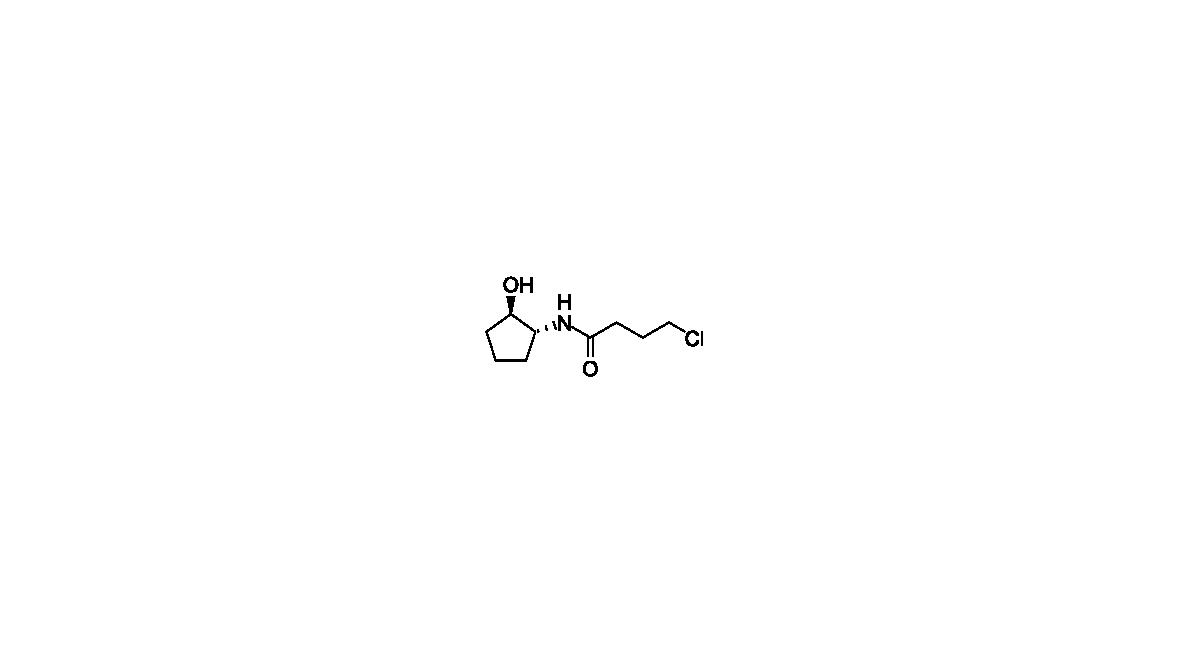
\includegraphics[scale=1]{HOcy5NH4Cl(RR).eps}
	\end{center}
\end{scheme}

(1\textit{R},2\textit{R})\hyp{}2\hyp{}Aminocyclopentan\hyp{}1\hyp{}ol \compound{cmpd:HOcy5NH2_RR} (500 mg, 4.94 mmol, 1 eq.), TEA (827 $\mu$l, 600 mg, 5.93 mmol, 1.2 eq.) and \ce{CH2Cl2} (20 ml) were stirred at 0 $^\circ$C and 4-chlorobutyryl chloride \compound{cmpd:Cl4Cl} (608 $\mu$l, 766 mg, 5.43 mmol, 1.1 eq.) was added dropwise over 5 min. The mixture was stirred at 0 $^\circ$C for 30 min, then water (50 ml) was added. The organic layer was separated off, and the aqueous layer was extracted with \ce{CH2Cl2} (7$\times$50 ml). The combined organic layers were dried with \ce{MgSO4}, concentrated under reduced pressure and purified by column chromatography (\ce{SiO2}, \ce{Et2O}). The combined pure fractions were dried with \ce{MgSO4} and evaporated under reduced pressure. \compound{cmpd:HOcy5NH4Cl_RR} was obtained as a white amorphous solid (651 mg, 3.16 mmol, 64.1 \%).
\\[1\baselineskip]
\noindent{\textbf{TLC} \textit{R$_f$} = 0.35 (EtOAc)}
\\[1\baselineskip]
%\noindent{\textbf{mp} \textit{T} / $^{\circ}$C = ?? (??)}
%\\[1\baselineskip]
\noindent{\textbf{IR} (neat) $\nu_{max}$ / cm$^{-1}$ = 
	3277.6 (N-H and O-H),
	2962.2 (C-H),
	2876.0 (C-H),
	1636.3 (amide C=O)}
\\[1\baselineskip]
\noindent{\textbf{$^{1}$H NMR} (400 MHz, \ce{CDCl3}) $\delta$ / ppm =
	6.12 (br s, 1 H, N\underline{H}), 
	4.42 (br s, 1 H, O\underline{H}), 
	3.94 (q, \textit{J} = 6.6 Hz, 1 H, C\underline{H}OH), 
	3.82 (tt, \textit{J} = 8.4, 5.3 Hz, 1 H, C\underline{H}NH), 
	3.60 (t, \textit{J} = 6.2 Hz, 2 H, C\underline{H}$_2$Cl), 
	2.38 (t, \textit{J} = 7.2 Hz, 2 H, C\underline{H}$_2$C=O), 
	2.05 - 2.16 (m, 3 H, C\underline{H}HCHNH and C\underline{H}$_2$CH$_2$Cl), 
	1.96 - 2.04 (m, 1 H, C\underline{H}HCHOH), 
	1.74 - 1.85 (m, 1 H, C\underline{H}HCH$_2$CHOH), 
	1.58 - 1.73 (m, 2 H, CH\underline{H}CH$_2$CHOH and CH\underline{H}CHOH), 
	1.43 (dq, \textit{J} = 12.7, 8.3 Hz, 1 H, CH\underline{H}CHNH)}
\\[1\baselineskip]
\noindent{\textbf{$^{13}$C NMR} (101 MHz, \ce{CDCl3}) $\delta$ / ppm = 
	173.8 (\underline{C}=O), 
	79.4 (\underline{C}HOH), 
	60.6 (\underline{C}HNH), 
	44.4 (\underline{C}H$_2$Cl), 
	32.8 (\underline{C}H$_2$C=O), 
	32.4 (\underline{C}H$_2$CHOH), 
	30.1 (\underline{C}H$_2$CHNH), 
	28.0 (\underline{C}H$_2$CH$_2$Cl), 
	21.1 (\underline{C}H$_2$CH$_2$CHOH)}
\\[1\baselineskip]
\noindent{\textbf{HRMS} (ESI$^+$) \textit{m}/\textit{z} / Da = 228.0787, [M+Na]$^+$ found, [\ce{C9H16ClNNaO2}]$^+$ requires 228.0762}
\\[1\baselineskip]
\noindent{[\bm{$\alpha$}]$_D^{20}$ / $^{\circ}$10$^{-1}$cm$^2$g$^{-1}$ = -13.0 (\textit{c} / g(100 ml)$^{-1}$ = 0.5, MeOH)}
\\[1\baselineskip]
The compound has not been reported previously.

\subsection{4\hyp{}Chloro\hyp{}\textit{N}\hyp{}((1\textit{S},2\textit{S})\hyp{}2\hyp{}hydroxycyclopentyl)butanamide \compound{cmpd:HOcy5NH4Cl_SS}}

%LMO-3-020

\begin{scheme}[H]
	\begin{center}
		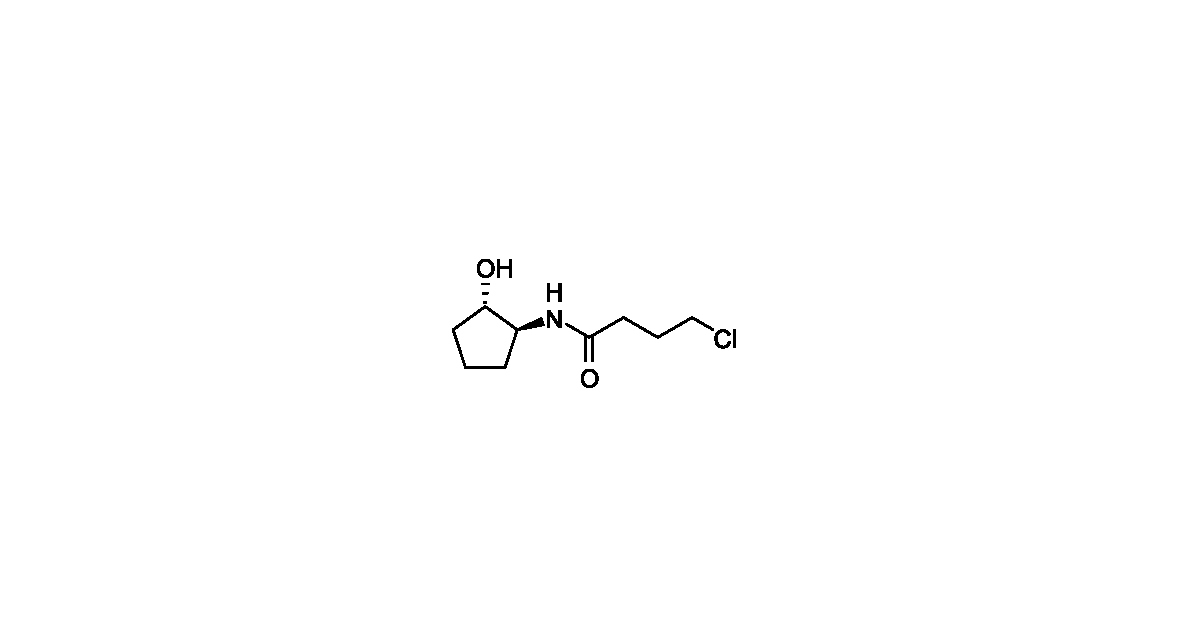
\includegraphics[scale=1]{HOcy5NH4Cl(SS).eps}
	\end{center}
\end{scheme}

(1\textit{S},2\textit{S})\hyp{}2\hyp{}Aminocyclopentan\hyp{}1\hyp{}ol \compound{cmpd:HOcy5NH2_SS} (72.3 mg, 716 $\mu$mol, 1 eq.), TEA (500 $\mu$l, 363 mg, 3.58 mmol, 5 eq.) and \ce{CH2Cl2} (5 ml) were stirred at 0 $^\circ$C, and 4-chlorobutyryl chloride \compound{cmpd:Cl4Cl} (179 $\mu$l, 226 mg, 1.60 mmol, 1.1 eq.) was added dropwise over 5 min. The mixture was stirred at 0 $^\circ$C for 30 min, then water (10 ml) was added. The organic layer was separated off, and the aqueous layer was extracted with 10 \% \textit{i}-PrOH/\ce{CHCl3} (2$\times$10 ml). The combined organic layers were dried with \ce{MgSO4}, concentrated under reduced pressure and purified by column chromatography (\ce{SiO2}, \ce{Et2O}). The combined pure fractions were dried with \ce{MgSO4} and evaporated under reduced pressure. \compound{cmpd:HOcy5NH4Cl_SS} was obtained as a white amorphous solid (35.6 mg, 173 $\mu$mol, 24.2 \%).%rough sm
\\[1\baselineskip]
\noindent{\textbf{TLC} \textit{R$_f$} = 0.35 (EtOAc)}
\\[1\baselineskip]
%\noindent{\textbf{mp} \textit{T} / $^{\circ}$C = ?? (??)}
%\\[1\baselineskip]
%\noindent{\textbf{IR} (neat) $\nu_{max}$ / cm$^{-1}$ = ??} 
%\\[1\baselineskip]
\noindent{\textbf{$^{1}$H NMR} (400 MHz, \ce{CDCl3}) $\delta$ / ppm = 
	6.05 (br s, 1 H, N\underline{H}), 
	4.55 (br s, 1 H, O\underline{H}), 
	3.95 (q, J=6.6 Hz, 1 H, C\underline{H}OH), 
	3.82 (tt, J=8.4, 5.3 Hz, 1 H, C\underline{H}NH), 
	3.60 (t, J=6.2 Hz, 2 H, C\underline{H}$_2$Cl), 
	2.38 (t, J=7.0 Hz, 2 H, C\underline{H}$_2$C=O), 
	2.05 - 2.17 (m, 3 H, C\underline{H}HCHNH and C\underline{H}$_2$CH$_2$Cl), 
	1.94 - 2.05 (m, 1 H, C\underline{H}HCHOH), 
	1.74 - 1.86 (m, 1 H, C\underline{H}HCH$_2$CHOH), 
	1.58 - 1.74 (m, 2 H, CH\underline{H}CH$_2$CHOH and CH\underline{H}CHOH), 
	1.42 (dq, J=12.5, 8.4 Hz, 1 H, CH\underline{H}CHNH)}
\\[1\baselineskip]
\noindent{\textbf{$^{13}$C NMR} (101 MHz, \ce{CDCl3}) $\delta$ / ppm = 
	173.8 (\underline{C}=O), 
	79.4 (\underline{C}HOH), 
	60.6 (\underline{C}HNH), 
	44.4 (\underline{C}H$_2$Cl), 
	32.8 (\underline{C}H$_2$C=O), 
	32.4 (\underline{C}H$_2$CHOH), 
	30.2 (\underline{C}H$_2$CHNH), 
	28.0 (\underline{C}H$_2$CH$_2$Cl), 
	21.2 (\underline{C}H$_2$CH$_2$CHOH)}
\\[1\baselineskip]
\noindent{\textbf{HRMS} (ESI$^+$) \textit{m}/\textit{z} / Da = 206.0939, [M+H]$^+$ found, [\ce{C9H17ClNO2}]$^+$ requires 206.0948}
\\[1\baselineskip]
\noindent{[\bm{$\alpha$}]$_D^{20}$ / $^{\circ}$10$^{-1}$cm$^2$g$^{-1}$ = 10.0 (\textit{c} / g(100 ml)$^{-1}$ = 0.05, MeOH)}
\\[1\baselineskip]
The compound has not been reported previously.

\subsection{4\hyp{}Azido\hyp{}\textit{N}\hyp{}((1\textit{S},2\textit{S})\hyp{}2\hyp{}((\textit{tert}\hyp{}butyldimethylsilyl)oxy)cyclopentyl)butanamide \compound{cmpd:TBSOcy5NH4N3_SS}}

%%LMO\hyp{}2\hyp{}074 (from dilute crude bromo, yes?), LMO\hyp{}2\hyp{}075 (from mixed fraction of 073), LMO\hyp{}2\hyp{}076 (more pooled mixed fractions, purified with 075, no mass recorded), LMO\hyp{}2\hyp{}077 (from mixed fractions, no mass recorded), LMO\hyp{}2\hyp{}078 (straight through from head group, columned with 075/6, worked)

\begin{scheme}[H]
	\begin{center}
		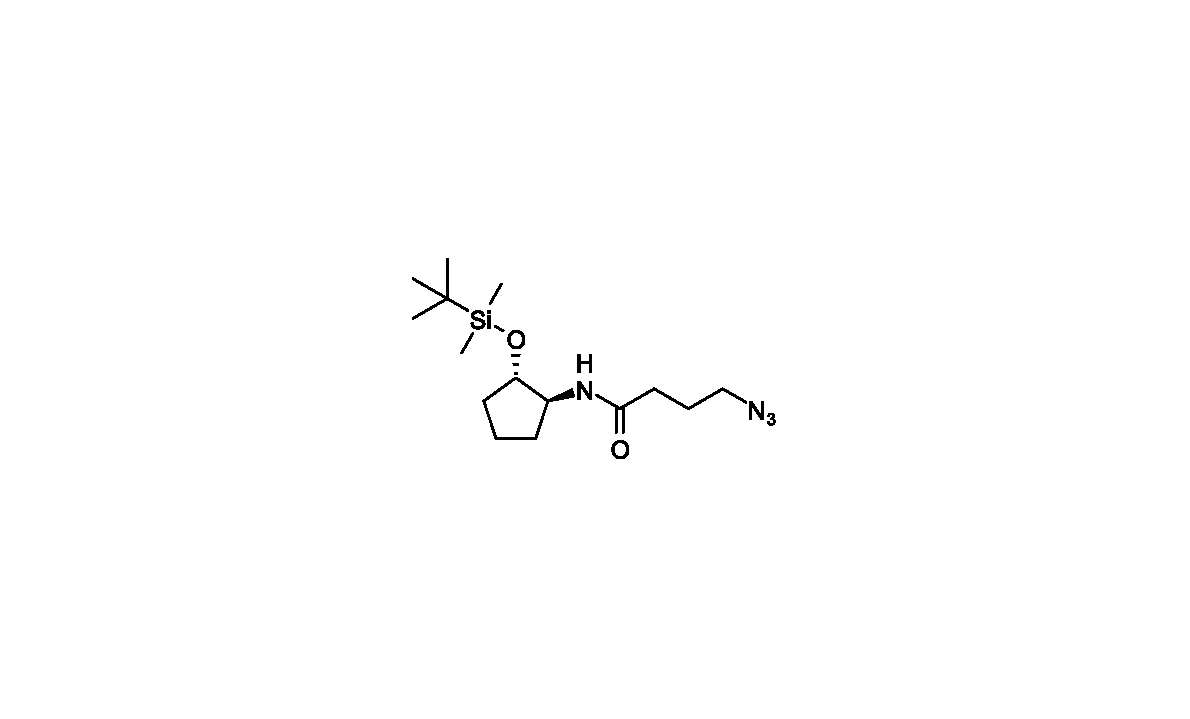
\includegraphics[scale=1]{TBSOcy5NH4N3(SS).eps}
	\end{center}
\end{scheme}
(1\textit{S},2\textit{S})\hyp{}2\hyp{}((\textit{tert}\hyp{}Butyldimethylsilyl)oxy)cyclopentan\hyp{}1\hyp{}amine \compound{cmpd:TBSOcy5NH2_SS} (50 mg, 0.232 mmol, 1 eq.) and \ce{NaHCO3} (22.0 mg, 0.262 mmol, 1.1 eq.) were added to \ce{CH2Cl2} (3 ml) and water (3 ml) at 0 $^\circ$C, and 4-bromobutyryl chloride (25.3 ml, 40.5 mg, 0.219 mmol, 0.95 eq.) was added dropwise. The mixture was stirred for 3 h at 0 $^\circ$C. The aqueous layer was removed and \ce{NaN3} (100 mg, 1.54 mmol, 6.6 eq.) and DMF (3 ml) were added. The mixture was then stirred at 40 $^\circ$C for 6 h. The solvents were then evaporated using a \ce{N2} stream and the residue was purified by column chromatography (\ce{SiO2}, 0.5 \% MeOH/\ce{CH2Cl2}). The combined pure fractions were dried with \ce{MgSO4} and evaporated under reduced pressure. \compound{cmpd:TBSOcy5NH4N3_SS} was obtained as a clear liquid (71 mg, 0.217 mmol, 99.2 \%).
\\[1\baselineskip]
\noindent{\textbf{TLC} \textit{R$_f$} = 0.84 (1 \% MeOH/\ce{CH2Cl2})}
\\[1\baselineskip]
%\noindent{\textbf{mp} \textit{T} / $^{\circ}$C = ?? (??)}
%\\[1\baselineskip]
\noindent{\textbf{IR} (neat) $\nu_{max}$ / cm$^{-1}$ = 
	3287.9 (N-H),
	2953.4 (C-H),
	2933.2 (C-H),
	2882.7 (C-H),
	2857.1 (C-H),
	2094.9 (azide),
	1639.4 (amide C=O)}
\\[1\baselineskip]
\noindent{\textbf{$^{1}$H NMR} (400 MHz, \ce{CDCl3}) $\delta$ / ppm =
	5.35 (d, \textit{J} = 5.1 Hz, 1 H, N\underline{H}), 
	3.97 - 4.01 (m, 1 H, C\underline{H}OSi), 
	3.93 - 3.98 (m, 1 H, C\underline{H}NH), 
	3.35 (t, \textit{J} = 6.6 Hz, 2 H, C\underline{H}$_2$N$_3$), 
	2.24 (t, \textit{J} = 7.0 Hz, 2 H, C\underline{H}$_2$C=O), 
	2.09 - 2.19 (m, 1 H, C\underline{H}HCHNH), 
	1.89 - 1.97 (quin, \textit{J} = 6.8 Hz, 2 H, C\underline{H}$_2$CH$_2$N$_3$), 
	1.74 - 1.84 (m, 2 H, C\underline{H}HCHOSi and C\underline{H}HCH$_2$CHOSi), 
	1.60 - 1.70 (m, 1 H, CH\underline{H}CH$_2$CHOSi), 
	1.51 - 1.61 (m, 1 H, CH\underline{H}CHOSi), 
	1.31 - 1.39 (m, 1 H, CH\underline{H}CHNH), 
	0.87 (s, 9 H, C(C\underline{H}$_3$)$_3$), 
	0.08 (s, 3 H, SiC\underline{H}$_3$), 
	0.06 (s, 3 H, SiC\underline{H}$_3$)}
\\[1\baselineskip]
\noindent{\textbf{$^{13}$C NMR} (101 MHz, \ce{CDCl3}) $\delta$ / ppm = 
	171.17 (\underline{C}=O), 
	77.80 (\underline{C}HOSi), 
	58.36 (\underline{C}HNH), 
	50.77 (\underline{C}H$_2$N$_3$), 
	33.29 (\underline{C}H$_2$C=O), 
	32.57 (\underline{C}H$_2$CHOSi), 
	29.36 (\underline{C}H$_2$CHNH), 
	25.72 (C(\underline{C}H$_3$)$_3$), 
	24.77 (\underline{C}H$_2$CH$_2$N$_3$), 
	20.40 (\underline{C}H$_2$CH$_2$CHO\allowbreak Si), 
	17.95 (\underline{C}(CH$_3$)$_3$), 
	-4.75 (Si\underline{C}H$_3$)}
\\[1\baselineskip]
\noindent{\textbf{HRMS} (ESI$^+$) \textit{m}/\textit{z} / Da = 327.2221, [M+H]$^+$ found, [\ce{C15H31N4O2Si}]$^+$ requires 327.2216}
\\[1\baselineskip]
\noindent{[\bm{$\alpha$}]$_D^{20}$ / $^{\circ}$10$^{-1}$cm$^2$g$^{-1}$ = 12.4 (\textit{c} / g(100 ml)$^{-1}$ = 0.5, MeOH)}
\\[1\baselineskip]
The compound has not been reported previously.

\subsection{4\hyp{}Azido\hyp{}\textit{N}\hyp{}((1\textit{R},2\textit{R})\hyp{}2\hyp{}hydroxycyclopentyl)butanamide \compound{cmpd:HOcy5NH4N3_RR}}

%%LMO\hyp{}2\hyp{}095 (done), LMO\hyp{}3\hyp{}002 (done)

\begin{scheme}[H]
	\begin{center}
		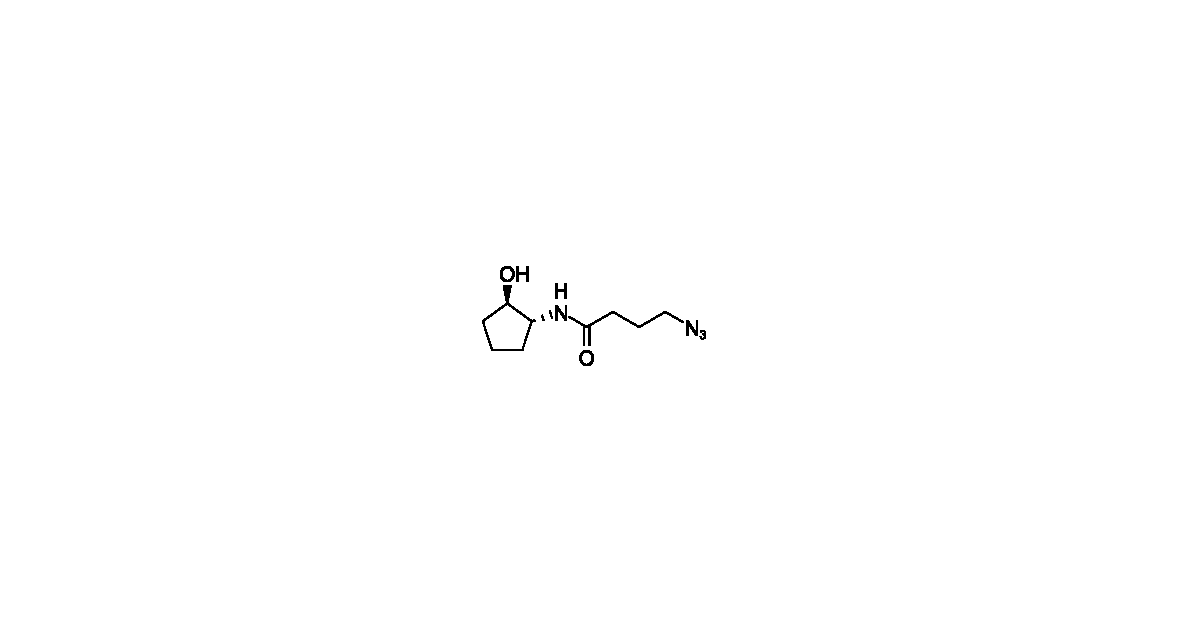
\includegraphics[scale=1]{HOcy5NH4N3(RR).eps}
	\end{center}
\end{scheme}

4\hyp{}Chloro\hyp{}\textit{N}\hyp{}((1\textit{R},2\textit{R})\hyp{}2\hyp{}hydroxycyclopentyl)butanamide \compound{cmpd:HOcy5NH4Cl_RR} (200 mg, 0.972 mmol, 1 eq.) and \ce{NaN3} (126 mg, 1.94 mmol, 2 eq.) were stirred in acetonitrile (4 ml) at 50 $^\circ$C for 16 h. The solvent was then evaporated under reduced pressure and the residue was partitioned between water (20 ml) and 10 \% \textit{i}-PrOH/\ce{CHCl3} (20 ml). The aqueous layer was extracted again with 10 \% \textit{i}-PrOH/\ce{CHCl3} (3$\times$20 ml) and the combined organic fractions were dried with \ce{MgSO4} and evaporated under reduced pressure. \compound{cmpd:HOcy5NH4N3_RR} was obtained as white needles (181 mg, 0.852 mmol, 87.6 \%).
\\[1\baselineskip]
\noindent{\textbf{TLC} \textit{R$_f$} = 0.35 (EtOAc)} %est. not useful.
\\[1\baselineskip]
\noindent{\textbf{mp} \textit{T} / $^{\circ}$C = 56.0-59.5 (\textit{i}-PrOH, \ce{CHCl3})}
\\[1\baselineskip]
\noindent{\textbf{IR} (neat) $\nu_{max}$ / cm$^{-1}$ = 
	3279.9 (N-H and O-H),
	2965.6 (C-H),
	2875.4 (C-H),
	2094.6 (azide),
	1636.8 (amide C=O)}
\\[1\baselineskip]
\noindent{\textbf{$^{1}$H NMR} (400 MHz, \ce{CDCl3}) $\delta$ / ppm =
	6.72 (d, \textit{J} = 4.4 Hz, 1 H, N\underline{H}), 
	4.82 (br. s., 1 H, O\underline{H}), 
	3.88 (q, \textit{J} = 6.6 Hz, 1 H, C\underline{H}OH), 
	3.75 (tdd, \textit{J} = 8.4, 8.4, 6.6, 4.4 Hz, 1 H, C\underline{H}NH), 
	3.28 (t, \textit{J} = 6.6 Hz, 2 H, C\underline{H}$_2$N$_3$), 
	2.23 (t, \textit{J} = 7.3 Hz, 2 H, C\underline{H}$_2$C=O), 
	2.04 (dtd, \textit{J} = 13.0, 8.0, 8.0, 4.9 Hz, 1 H, C\underline{H}HCHNH), 
	1.92 (dtd, \textit{J} = 13.0, 7.6, 7.6, 5.8 Hz, 1 H, C\underline{H}HCHOH), 
	1.84 (quin, \textit{J} = 7.0 Hz, 2 H, C\underline{H}$_2$CH$_2$N$_3$), 
	1.59 - 1.77 (m, 2 H, C\underline{H}$_2$CH$_2$CHOH), 
	1.54 (ddt, \textit{J} = 12.7, 9.0, 6.7, 6.7 Hz, 1 H, CH\underline{H}CHOH), 
	1.39 (dq, \textit{J} = 12.9, 8.4 Hz, 1 H, CH\underline{H}CHNH)}
\\[1\baselineskip]
\noindent{\textbf{$^{13}$C NMR} (101 MHz, \ce{CDCl3}) $\delta$ / ppm = 
	173.8 (\underline{C}=O), 
	78.8 (\underline{C}HOH), 
	59.9 (\underline{C}HNH), 
	50.5 (\underline{C}H$_2$N$_3$), 
	32.5 (\underline{C}H$_2$C=O), 
	32.0 (\underline{C}H$_2$CHOH), 
	29.5 (\underline{C}H$_2$CHNH), 
	24.6 (\underline{C}H$_2$CH$_2$N$_3$), 
	20.7 (\underline{C}H$_2$CH$_2$CHOH)}
\\[1\baselineskip]
\noindent{\textbf{HRMS} (ESI$^+$) \textit{m}/\textit{z} / Da = 235.1174, [M+Na]$^+$ found, [\ce{C9H16N4NaO2}]$^+$ requires 235.1171}
\\[1\baselineskip]
\noindent{[\bm{$\alpha$}]$_D^{20}$ / $^{\circ}$10$^{-1}$cm$^2$g$^{-1}$ = -10.2 (\textit{c} / g(100 ml)$^{-1}$ = 0.5, MeOH)}
\\[1\baselineskip]
The compound has not been reported previously.

\subsection{4\hyp{}Azido\hyp{}\textit{N}\hyp{}((1\textit{S},2\textit{S})\hyp{}2\hyp{}hydroxycyclopentyl)butanamide \compound{cmpd:HOcy5NH4N3_SS}} 

%LMO-3-021, LMO-3-023

\begin{scheme}[H]
	\begin{center}
		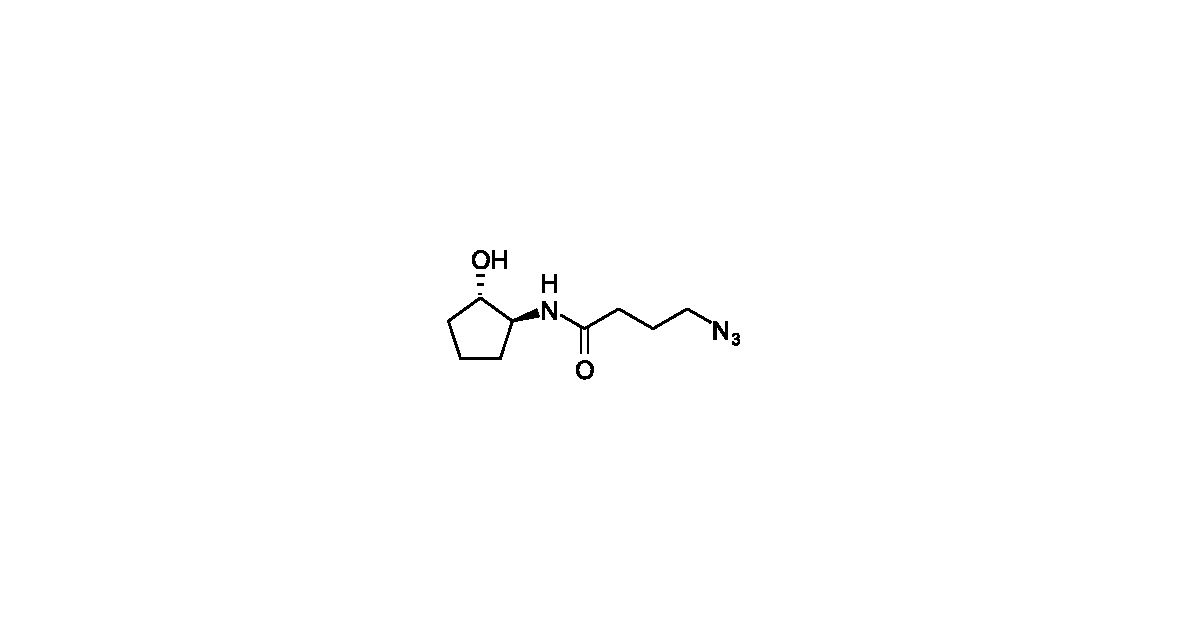
\includegraphics[scale=1]{HOcy5NH4N3(SS).eps}
	\end{center}
\end{scheme}

4\hyp{}Chloro\hyp{}\textit{N}\hyp{}((1\textit{S},2\textit{S})\hyp{}2\hyp{}hydroxycyclopentyl)butanamide \compound{cmpd:HOcy5NH4Cl_SS} (35.0 mg, 0.170 mmol, 1 eq.) and \ce{NaN3} (22.1 mg, 0.340 mmol, 2 eq.) were stirred in acetonitrile (2 ml) at 50 $^\circ$C for 24 h. The reaction mixture was then partitioned between water (20 ml) and 10 \% \textit{i}-PrOH/\ce{CHCl3} (5 ml). The aqueous layer was extracted again with 10 \% \textit{i}-PrOH/\ce{CHCl3} (2$\times$5 ml) and the combined organic fractions were dried with \ce{MgSO4} and evaporated under reduced pressure. \compound{cmpd:HOcy5NH4N3_SS} was obtained as white needles (16.2 mg, 0.0764 mmol, 45.0 \%).
\\[1\baselineskip]
\noindent{\textbf{TLC} \textit{R$_f$} = 0.35 (EtOAc)} %est
\\[1\baselineskip]
%\noindent{\textbf{mp} \textit{T} / $^{\circ}$C = ?? (??)} not enough
%\\[1\baselineskip]
\noindent{\textbf{IR} (neat) $\nu_{max}$ / cm$^{-1}$ = 
	3286.7 (N-H and O-H),
	2957.6 (C-H),
	2930.6 (C-H),
	2860.7 (C-H),
	2094.7 (azide),
	1642.2 (amide C=O)}
\\[1\baselineskip]
\noindent{\textbf{$^{1}$H NMR} (400 MHz, \ce{CDCl3}) $\delta$ / ppm = 
	5.82 (br s, 1 H, N\underline{H}), 
	4.45 (br. s., 1 H, O\underline{H}), 
	3.96 (q, J=6.6 Hz, 1 H, C\underline{H}OH), 
	3.83 (tdd, J=8.5, 8.5, 6.0, 4.6 Hz, 1 H, C\underline{H}NH), 
	3.37 (t, J=6.4 Hz, 2 H, C\underline{H}$_2$N$_3$), 
	2.31 (t, J=7.2 Hz, 2 H, C\underline{H}$_2$C=O), 
	2.09 - 2.19 (m, 1 H, C\underline{H}HCHNH), 
	1.99 - 2.06 (m, 1 H, C\underline{H}HCHOH), 
	1.90 - 1.97 (m, 2 H, C\underline{H}$_2$CH$_2$N$_3$), 
	1.60 - 1.85 (m, 3 H, C\underline{H}$_2$CH\underline{H}CHOH), 
	1.42 (dq, J=12.8, 8.3 Hz, 1 H, CH\underline{H}CHNH)}
\\[1\baselineskip]
\noindent{\textbf{$^{13}$C NMR} (101 MHz, \ce{CDCl3}) $\delta$ / ppm = 
	173.8 (\underline{C}=O), 
	79.7 (\underline{C}HOH), 
	61.0 (\underline{C}HNH), 
	50.7 (\underline{C}H$_2$N$_3$), 
	32.8 (\underline{C}H$_2$C=O), 
	32.6 (\underline{C}H$_2$CHOH), 
	30.5 (\underline{C}H$_2$CHNH), 
	24.7 (\underline{C}H$_2$CH$_2$N$_3$), 
	21.3 (\underline{C}H$_2$CH$_2$CHOH)}
\\[1\baselineskip]
\noindent{\textbf{HRMS} (ESI$^+$) \textit{m}/\textit{z} / Da = 235.1178, [M+Na]$^+$ found, [\ce{C9H16N4NaO2}]$^+$ requires 235.1171}
\\[1\baselineskip]
\noindent{[\bm{$\alpha$}]$_D^{20}$ / $^{\circ}$10$^{-1}$cm$^2$g$^{-1}$ = 10.0 (\textit{c} / g(100 ml)$^{-1}$ = 0.01, MeOH)}
\\[1\baselineskip]
The compound has not been reported previously.


%\subsection{Methyl 7\hyp{}(4\hyp{}(4\hyp{}(((1\textit{R},2\textit{R})\hyp{}2\hyp{}((\textit{tert}\hyp{}butyldimethylsilyl)oxy)cyclopentyl)amino)\hyp{}4\hyp{}oxobutyl)piperazin\hyp{}1\hyp{}yl)\hyp{}1\hyp{}cyclopropyl\hyp{}6\hyp{}fluoro\hyp{}4\hyp{}oxo\hyp{}1,4\hyp{}dihydroquinoline\hyp{}3\hyp{}carboxylate \compound{cmpd:TBSOcy5NH4CipMe(RR)}}
%
%%%LMO\hyp{}2\hyp{}086 (slow, not used?)
%
%\begin{scheme}[H]
%	\begin{center}
%		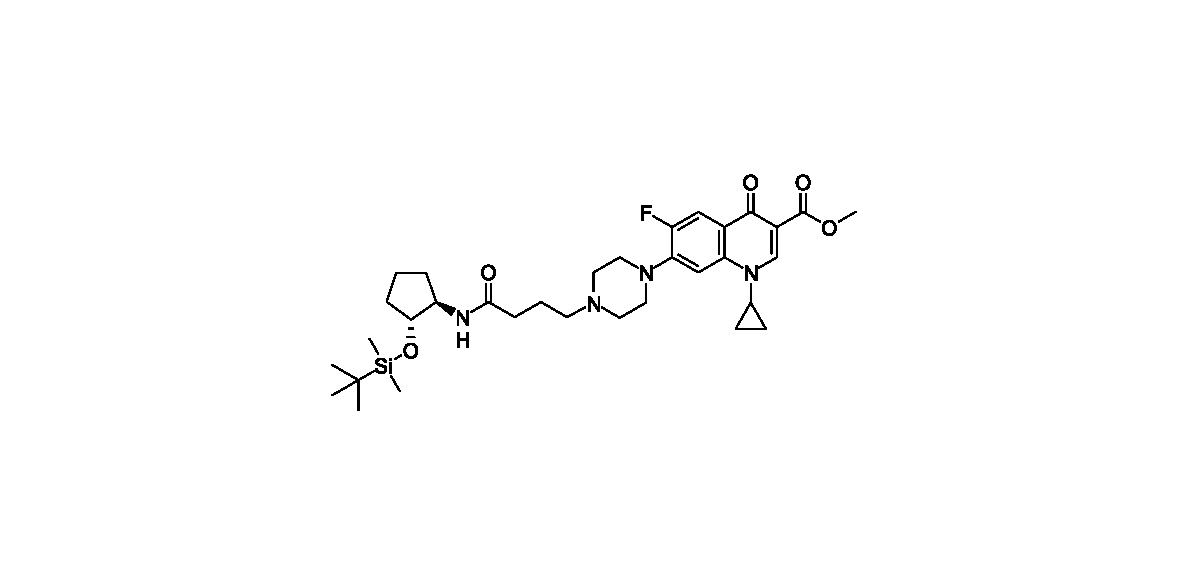
\includegraphics[scale=1]{TBSOcy5NH4CipMe(RR).eps}
%	\end{center}
%\end{scheme}

\subsection{Methyl 1\hyp{}cyclopropyl\hyp{}6\hyp{}fluoro\hyp{}7\hyp{}(4\hyp{}(4\hyp{}(((1\textit{R},2\textit{R})\hyp{}2\hyp{}hydroxycyclopentyl)amin\allowbreak o)\hyp{}4\hyp{}oxobutyl)piperazin\hyp{}1\hyp{}yl)\hyp{}4\hyp{}oxo\hyp{}1,4\hyp{}dihydroquinoline\hyp{}3\hyp{}carboxylate \compound{cmpd:HOcy5NH4CipMe_RR}}

%%LMO\hyp{}3\hyp{}003 (SN2 method, messy, chucked), LMO\hyp{}2\hyp{}091 (done, worked up but HOBt contamination after column), LMO\hyp{}2\hyp{}093 (done)

\begin{scheme}[H]
	\begin{center}
		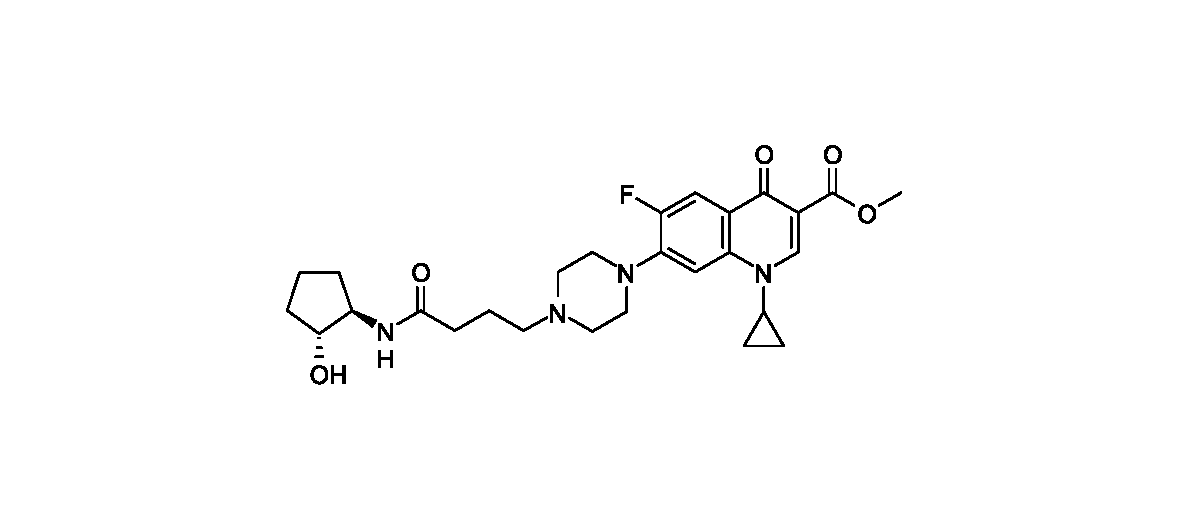
\includegraphics[scale=1]{HOcy5NH4CipMe(RR).eps}
	\end{center}
\end{scheme}

4\hyp{}(4\hyp{}(1\hyp{}Cyclopropyl\hyp{}6\hyp{}fluoro\hyp{}3\hyp{}(methoxycarbonyl)\hyp{}4\hyp{}oxo\hyp{}1,4\hyp{}dihydroquinolin\hyp{}7\hyp{}yl)piperazin\hyp{}1\hyp{}yl)butanoic\hfill acid trifluoroacetate \compound{cmpd:HOO4CipMeTFA} (200 mg, 0.367 mmol, 1 eq.), (1\textit{R},2\textit{R})\hyp{}2\hyp{}aminocyclopentan\hyp{}1\hyp{}ol \compound{cmpd:HOcy5NH2_RR} (80 mg, 0.791 mmol, 2.1 eq.), 1-ethyl-3-(3-dimethylaminopropyl)carbodiimide hydrochloride (112 mg, 0.584 mmol, 1.6 eq.), 1-hydroxyben\allowbreak zotriazole (96 mg, 0.710 mmol, 1.9 eq.) and DIPEA (192 $\mu$l, 142 mg, 1.10 mmol, 3 eq.) were dissolved in DMF (5 ml) and stirred at r.t. for 16 h. The solvent was removed using a stream of \ce{N2} and the residue was purified by preparatory HPLC (5-60 \% acetonitrile/water over 12 min). The combined pure fractions were evaporated under reduced pressure and then partitioned between \ce{NaHCO3} (aq., sat., 10 ml) and \ce{CH2Cl2} (10 ml). The organic layer was removed and the aqueous layer was extracted twice more with \ce{CH2Cl2} (2$\times$10 ml). The combined organic fractions were dried with \ce{MgSO4} and evaporated under reduced pressure. \compound{cmpd:HOcy5NH4CipMe_RR} was obtained as a white amorphous solid (73.0 mg, 0.142 mmol, 38.7 \%).
\\[1\baselineskip]
\noindent{\textbf{TLC} \textit{R$_f$} = 0.43 (30 \% MeOH/EtOAc)}
\\[1\baselineskip]
%\noindent{\textbf{mp} \textit{T} / $^{\circ}$C = ?? (??)}
%\\[1\baselineskip]
\noindent{\textbf{IR} (neat) $\nu_{max}$ / cm$^{-1}$ = 
	2972.9 (C-H),
	2901.5 (C-H),
	1728.4 (ester C=O),
	1656.3 (amide C=O),
	1612.9 (quinolone C=O)}
\\[1\baselineskip]
\noindent{\textbf{$^{1}$H NMR} (400 MHz, DMSO d$_6$) $\delta$ / ppm = 
	8.44 (s, 1 H, \textit{ortho} to C(=O)OC\underline{H}$_3$), 
	7.75 (d, \textit{J} = 13.5 Hz, 1 H, \textit{ortho} to F), 
	7.70 (d, \textit{J} = 7.2 Hz, 1 H, CHN\underline{H}), 
	7.43 (d, \textit{J} = 7.5 Hz, 1 H, \textit{meta} to F), 
	4.74 (d, \textit{J} = 4.0 Hz, 1 H, CHO\underline{H}), 
	3.78 - 3.82 (m, 1 H, C\underline{H}OH), 
	3.74 - 3.78 (m, 1 H, C\underline{H}NH), 
	3.74 (s, 3 H, C\underline{H}$_3$), 
	3.65 (tt, \textit{J} = 7.2, 3.9 Hz, 1 H, NC\underline{H}(CH$_2$)$_2$), 
	3.25 (t, \textit{J} = 4.8 Hz, 4 H, CH$_2$N(CH$_2$C\underline{H}$_2$)CH$_2$C\underline{H}$_2$), 
	2.57 (br s, 4 H, CH$_2$N(C\underline{H}$_2$)C\underline{H}$_2$), 
	2.34 (t, \textit{J} = 7.4 Hz, 2 H, C\underline{H}$_2$N(CH$_2$)CH$_2$), 
	2.11 (t, \textit{J} = 7.4 Hz, 2 H, C\underline{H}$_2$CH$_2$CH$_2$N(CH$_2$)CH$_2$), 
	1.92 (dddd, \textit{J} = 13.0, 8.7, 7.3, 6.0 Hz, 1 H, C\underline{H}HCHNH),
	1.78 (dddd, \textit{J} = 12.6, 8.9, 6.3, 6.3 Hz, 1 H, C\underline{H}HCHOH),  
	1.69 (quin, \textit{J} = 7.3 Hz, 2 H, C\underline{H}$_2$CH$_2$N(CH$_2$)CH$_2$), 
	1.54 - 1.65 (m, 2 H, C\underline{H}$_2$CH$_2$CHOH), 
	1.42 (ddt, \textit{J} = 13.1, 8.2, 5.3, 5.3 Hz, 1 H, CH\underline{H}CHOH), 
	1.32 (dddd, \textit{J} = 13.4, 8.5, 6.8, 5.8 Hz, 1 H, CH\underline{H}CHNH), 
	1.21 - 1.29 (m, 2 H, NCH(C\underline{H}H)$_2$), 
	1.07 - 1.13 (m, 2 H, NCH(CH\underline{H})$_2$)}
\\[1\baselineskip]
\noindent{\textbf{$^{13}$C NMR} (101 MHz, DMSO d$_6$) $\delta$ / ppm = 
	171.9 (CH$_2$\underline{C}(=O)NH), 
	171.6 (\underline{C}(=O)CC(=O)OCH$_3$), 
	165.0 (\underline{C}(=O)OCH$_3$), 
	152.6 (d, \textit{J} = 246.5 Hz, \textit{ipso} to F), 
	148.3 (\underline{C}=CC(=O)OCH$_3$), 
	143.9 (d, \textit{J} = 10.7 Hz, \textit{ipso} to piperazine), 
	138.1 (\textit{para} to F), 
	121.8 (d, \textit{J} = 6.4 Hz, \textit{para} to piperazine), 
	111.5 (d, \textit{J} = 22.4 Hz, \textit{ortho} to C=O and \textit{ortho} to F), 
	109.0 (\underline{C}C(=O)OCH$_3$), 
	106.2 (\textit{meta} to C=O and \textit{meta} to F), 
	76.3 (\underline{C}HOH), 
	57.6 (\underline{C}HNH), 
	57.2 (CH$_2$CH$_2$\underline{C}H$_2$N), 
	52.4 (CH$_2$CH$_2$CH$_2$N(\underline{C}H$_2$)\underline{C}H$_2$), 
	51.3 (\underline{C}H$_3$), 
	49.6 (CH$_2$CH$_2$CH$_2$N(CH$_2$\underline{C}H$_2$)CH$_2$\underline{C}H$_2$), 
	34.8 (N\underline{C}H(CH$_2$)$_2$), 
	33.3 (C(=O)\underline{C}H$_2$), 
	32.2 (\underline{C}H$_2$CHOH), 
	29.5 (\underline{C}H$_2$CHNH), 
	22.5 (C(=O)CH$_2$\underline{C}H$_2$), 
	20.6 (\underline{C}H$_2$CH$_2$CHOH), 
	7.6 (NCH(\underline{C}H$_2$)$_2$)}
\\[1\baselineskip]
\noindent{\textbf{$^{19}$F NMR} (376.45 MHz, DMSO d$_6$) $\delta$ / ppm = 
	-124.3 (ciprofloxacin F)}
\\[1\baselineskip]
\noindent{\textbf{HRMS} (ESI$^+$) \textit{m}/\textit{z} / Da = 515.2661, [M+H]$^+$ found, [\ce{C27H36FN4O5}]$^+$ requires 515.2670}
\\[1\baselineskip]
\noindent{[\bm{$\alpha$}]$_D^{20}$ / $^{\circ}$10$^{-1}$cm$^2$g$^{-1}$ = -6.0 (\textit{c} / g(100 ml)$^{-1}$ = 0.05, MeOH)}
\\[1\baselineskip]
The compound has not been reported previously.

\subsection{Methyl 1\hyp{}cyclopropyl\hyp{}6\hyp{}fluoro\hyp{}7\hyp{}(4\hyp{}(4\hyp{}(((1\textit{S},2\textit{S})\hyp{}2\hyp{}hydroxycyclopentyl)amin\allowbreak o)\hyp{}4\hyp{}oxobutyl)piperazin\hyp{}1\hyp{}yl)\hyp{}4\hyp{}oxo\hyp{}1,4\hyp{}dihydroquinoline\hyp{}3\hyp{}carboxylate \compound{cmpd:HOcy5NH4CipMe_SS}}

%%LMO\hyp{}2\hyp{}085 (peptide coupling, slow/stalled) LMO-3-019 (done)

\begin{scheme}[H]
	\begin{center}
		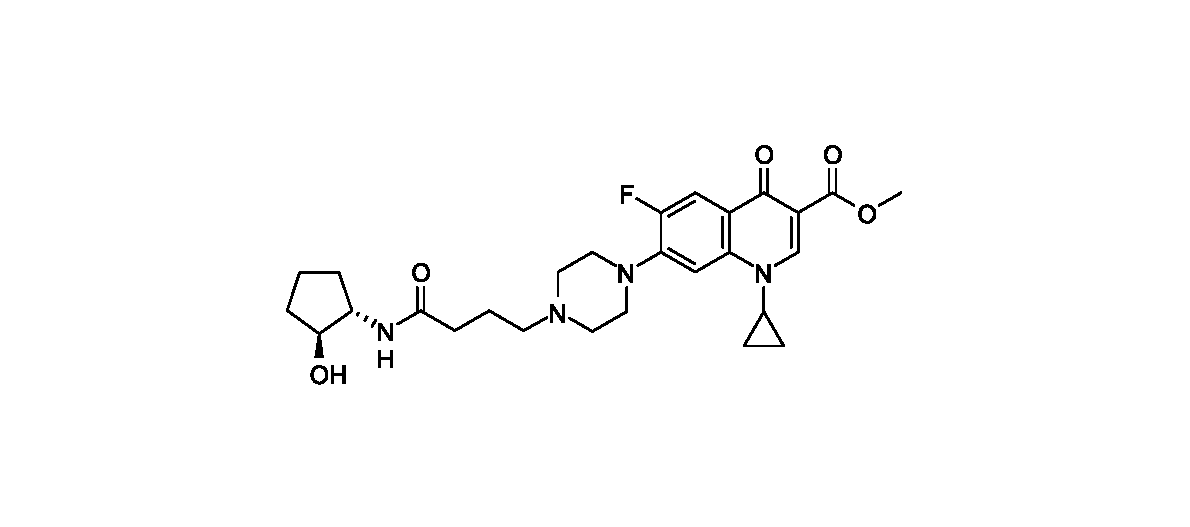
\includegraphics[scale=1]{HOcy5NH4CipMe(SS).eps}
	\end{center}
\end{scheme}

4\hyp{}(4\hyp{}(1\hyp{}Cyclopropyl\hyp{}6\hyp{}fluoro\hyp{}3\hyp{}(methoxycarbonyl)\hyp{}4\hyp{}oxo\hyp{}1,4\hyp{}dihydroquinolin\hyp{}7\hyp{}yl)piperazin\hyp{}1\hyp{}yl)butanoic\hfill acid trifluoroacetate \compound{cmpd:HOO4CipMeTFA} (52.1 mg, 95.5 $\mu$mol, 1 eq.), (1\textit{S},2\textit{S})\hyp{}2\hyp{}aminocyclopentan\hyp{}1\hyp{}ol \compound{cmpd:HOcy5NH2_SS} (19.5 mg, 193 $\mu$mol, 2 eq.), 1-ethyl-3-(3-dimethylaminopropyl)carbodiimide hydrochloride (29.7 mg, 155 $\mu$mol, 1.6 eq.), 1-hydroxyben\allowbreak zotriazole (25.8 mg, 191 $\mu$mol, 2 eq.) and DIPEA (33.3 $\mu$l, 24.7 mg, 191 $\mu$mol, 2 eq.) were dissolved in DMF (2 ml) and stirred at r.t. for 16 h. The solvent was removed using a stream of \ce{N2} and the residue was purified by preparatory HPLC (5-50 \% acetonitrile/water over 15 min). The combined pure fractions were evaporated under reduced pressure and then partitioned between \ce{NaHCO3} (aq., sat., 5 ml) and \ce{CH2Cl2} (5 ml). The organic layer was removed and the aqueous layer was extracted twice more with \ce{CH2Cl2} (2$\times$5 ml). The combined organic fractions were dried with \ce{MgSO4} and evaporated under reduced pressure. \compound{cmpd:HOcy5NH4CipMe_SS} was obtained as a white amorphous solid (4.9 mg, 9.5 $\mu$mol, 9.9 \%).
\\[1\baselineskip]
\noindent{\textbf{TLC} \textit{R$_f$} = 0.38 (30 \% MeOH/\ce{CH2Cl2})}
\\[1\baselineskip]
%\noindent{\textbf{mp} \textit{T} / $^{\circ}$C = ?? (??)}
%\\[1\baselineskip]
\noindent{\textbf{IR} (neat) $\nu_{max}$ / cm$^{-1}$ = 
	2937.7 (C-H),
	1721.4 (ester C=O),
	1620.5 (amide C=O and quinolone C=O)}
\\[1\baselineskip]
\noindent{\textbf{$^{1}$H NMR} (500 MHz, DMSO d$_6$) $\delta$ / ppm = 
	8.44 (s, 1 H, \textit{ortho} to C(=O)OC\underline{H}$_3$), 
	7.75 (d, J=13.5 Hz, 1 H, \textit{ortho} to F), 
	7.69 (d, J=6.9 Hz, 1 H, CHN\underline{H}), 
	7.43 (d, J=7.6 Hz, 1 H, \textit{meta} to F), 
	4.73 (br s, 1 H, CHO\underline{H}), 
	3.77 - 3.81 (m, 1 H, C\underline{H}OH), 
	3.74 - 3.77 (m, 1 H, C\underline{H}NH), 
	3.73 (s, 3 H, C\underline{H}$_3$), 
	3.65 (tt, J=6.9, 4.0 Hz, 1 H, NC\underline{H}(CH$_2$)$_2$), 
	3.24 (br. t, J=4.2, 4.2 Hz, 4 H, CH$_2$N(CH$_2$C\underline{H}$_2$)CH$_2$C\underline{H}$_2$), 
	2.55 (br t, J=5.0, 5.0 Hz, 4 H, CH$_2$N(C\underline{H}$_2$)C\underline{H}$_2$), 
	2.32 (t, J=7.2 Hz, 2 H, C\underline{H}$_2$N(CH$_2$)CH$_2$), 
	2.10 (t, J=7.4 Hz, 2 H, C\underline{H}$_2$CH$_2$CH$_2$N(CH$_2$)CH$_2$), 
	1.92 (dddd, J=13.0, 8.7, 7.3, 6.0 Hz, 1 H, C\underline{H}HCHNH), 
	1.77 (ddt, J=12.6, 8.9, 6.3, 6.3 Hz, 1 H, C\underline{H}HCHOH), 
	1.68 (quin, J=7.4 Hz, 2 H, C\underline{H}$_2$CH$_2$N(CH$_2$)CH$_2$), 
	1.53 - 1.64 (m, 2 H, C\underline{H}$_2$CH$_2$CHOH), 
	1.42 (ddt, J=12.9, 8.4, 5.2, 5.2 Hz, 1 H, CH\underline{H}CHOH), 
	1.31 (ddt, J=13.0, 8.6, 6.4, 6.4 Hz, 1 H, CH\underline{H}CHNH), 
	1.22 - 1.28 (m, 2 H, NCH(C\underline{H}H)$_2$), 
	1.06 - 1.12 (m, 2 H, NCH(CH\underline{H})$_2$)}
\\[1\baselineskip]
\noindent{\textbf{$^{13}$C NMR} (126 MHz, DMSO d$_6$) $\delta$ / ppm = 
	171.9 (NH\underline{C}(=O)CH$_2$), 
	171.5 (\underline{C}(=O)CC(=O)OCH$_3$), 
	165.0 (\underline{C}(=O)OCH$_3$), 
	152.6 (d, J=247.4 Hz, \textit{ipso} to F), 
	148.2 (\underline{C}=CC(=O)OCH$_3$), 
	143.9 (d, J=10.3 Hz, \textit{ipso} to piperazine), 
	138.1 (\textit{para} to F), 
	121.7 (d, J=6.4 Hz, \textit{para} to piperazine), 
	111.5 (d, J=23.0 Hz, \textit{ortho} to C=O and \textit{ortho} to F), 
	109.0 (\underline{C}C(=O)OCH$_3$), 
	106.2 (\textit{meta} to C=O and \textit{meta} to F), 
	76.2 (\underline{C}HOH), 
	57.6 (\underline{C}HNH), 
	57.2 (CH$_2$CH$_2$\underline{C}H$_2$N), 
	52.4 (CH$_2$CH$_2$CH$_2$N(\underline{C}H$_2$)\underline{C}H$_2$), 
	51.3 (\underline{C}H$_3$), 
	49.6 (CH$_2$CH$_2$CH$_2$N(CH$_2$\underline{C}H$_2$)CH$_2$CH$_2$), 
	49.6 (CH$_2$CH$_2$CH$_2$N(CH$_2$CH$_2$)CH$_2$\underline{C}H$_2$), 
	34.7 (N\underline{C}H(CH$_2$)$_2$), 
	33.2 (C(=O)\underline{C}H$_2$), 
	32.2 (\underline{C}H$_2$CHOH), 
	29.5 (\underline{C}H$_2$CH\allowbreak NH), 
	22.5 (C(=O)CH$_2$\underline{C}H$_2$), 
	20.6 (\underline{C}H$_2$CH$_2$CHOH), 
	7.5 (NCH(\underline{C}H$_2$)$_2$)}
\\[1\baselineskip]
\noindent{\textbf{$^{19}$F NMR} (376.45 MHz, MeOD) $\delta$ / ppm = 
	-125.5}%\todo{still TFA present after desalt attempt}}
\\[1\baselineskip]
\noindent{\textbf{HRMS} (ESI$^+$) \textit{m}/\textit{z} / Da = 515.2667, [M+H]$^+$ found, [\ce{C27H36FN4O5}]$^+$ requires 515.2670}
\\[1\baselineskip]
\noindent{[\bm{$\alpha$}]$_D^{20}$ / $^{\circ}$10$^{-1}$cm$^2$g$^{-1}$ = 8.0 (\textit{c} / g(100 ml)$^{-1}$ = 0.05, MeOH)}
\\[1\baselineskip]
The compound has not been reported previously.
		
	
% \todo{this is for the salt}
% 175.4 (\underline{C}(=O)CC(=O)OCH$_3$), 
% 175.2 (CH$_2$\underline{C}(=O)NH), 
% 166.8 (\underline{C}(=O)OCH$_3$), 
% 154.9 (d, \textit{J} = 248.0 Hz, \textit{ipso} to F), 
% 150.5 (\underline{C}=CC(=O)OCH$_3$), 
% 144.6 (d, \textit{J} = 10.7 Hz, \textit{ipso} to piperazine), 
% 140.0 (\textit{para} to F), 
% 124.6 (br s, \textit{para} to piperazine), 
% 113.6 (d, \textit{J} = 22.4 Hz, \textit{ortho} to C=O and \textit{ortho} to F), 
% 110.4 (\underline{C}C(=O)OCH$_3$), 
% 108.1 (\textit{meta} to C=O and \textit{meta} to F), 
% 78.6 (\underline{C}HOH), 
% 59.6 (\underline{C}HNH), 
% 58.4 (C(=O)CH$_2$CH$_2$\underline{C}H$_2$N), 
% 53.1 (C(=O)CH$_2$CH$_2$CH$_2$N(\underline{C}H$_2$)\underline{C}H$_2$), 
% 52.4 (\underline{C}H$_3$), 
% 48.3 (C(=O)CH$_2$CH$_2$CH$_2$N(CH$_2$\underline{C}H$_2$)CH$_2$\underline{C}H$_2$), 
% 36.5 (N\underline{C}H(CH$_2$)$_2$), 
% 34.3 (C(=O)\underline{C}H$_2$), 
% 33.3 (\underline{C}H$_2$CHOH), 
% 30.5 (\underline{C}H$_2$CHNH), 
% 21.7 (\underline{C}H$_2$CH$_2$CHOH), 
% 21.0 (C(=O)CH$_2$\underline{C}H$_2$), 
% 8.7 (NCH(\underline{C}H$_2$)$_2$)
% 
% F
% 
% -77.0 (C\underline{F}$_3$), 
% -125.4 (ciprofloxacin F)

%\subsection{methyl (\textit{S})\hyp{}1\hyp{}cyclopropyl\hyp{}6\hyp{}fluoro\hyp{}4\hyp{}oxo\hyp{}7\hyp{}(4\hyp{}(4\hyp{}oxo\hyp{}4\hyp{}((2\hyp{}oxocyclopentyl)am\hyp{}ino)butyl)piperazin\hyp{}1\hyp{}yl)\hyp{}1,4\hyp{}dihydroquinoline\hyp{}3\hyp{}carboxylate \compound{cmpd:Ocy5NH4CipMe(S)}}
%
%%%LMO\hyp{}3\hyp{}005 (DMF, Bayer\hyp{}Villager, chucked)
%
%\begin{scheme}[H]
%	\begin{center}
%		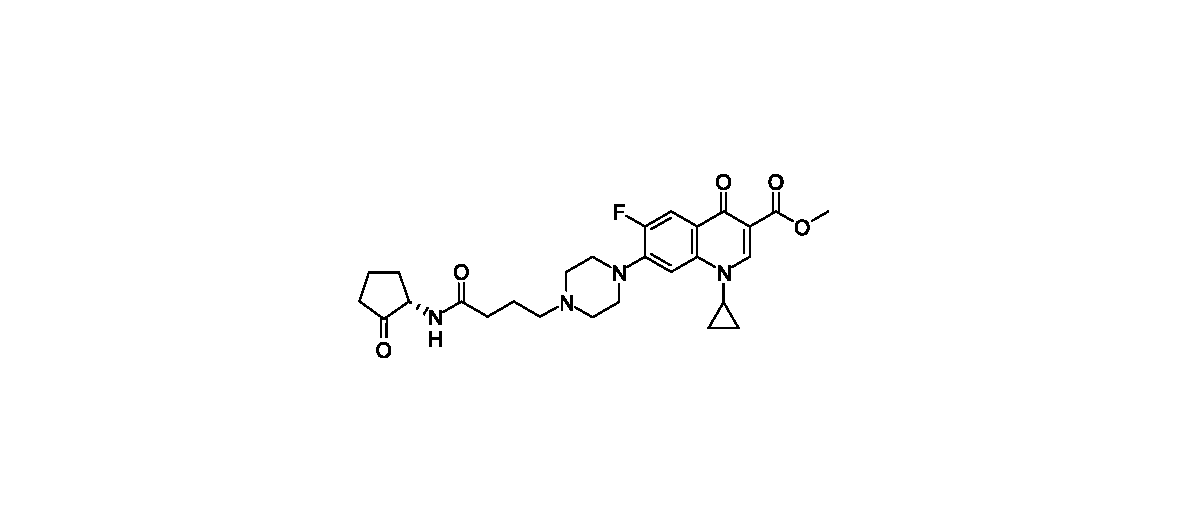
\includegraphics[scale=1]{Ocy5NH4CipMe(S).eps}
%	\end{center}
%\end{scheme}

%\subsection{Methyl (\textit{S})\hyp{}1\hyp{}cyclopropyl\hyp{}6\hyp{}fluoro\hyp{}4\hyp{}oxo\hyp{}7\hyp{}(4\hyp{}(4\hyp{}oxo\hyp{}4\hyp{}((2\hyp{}oxocyclopentyl)am\hyp{}ino)butyl)piperazin\hyp{}1\hyp{}yl)\hyp{}1,4\hyp{}dihydroquinoline\hyp{}3\hyp{}carboxylate \compound{cmpd:Ocy5NH4CipMe(S)}}
%
%\begin{scheme}[H]
%	\begin{center}
%		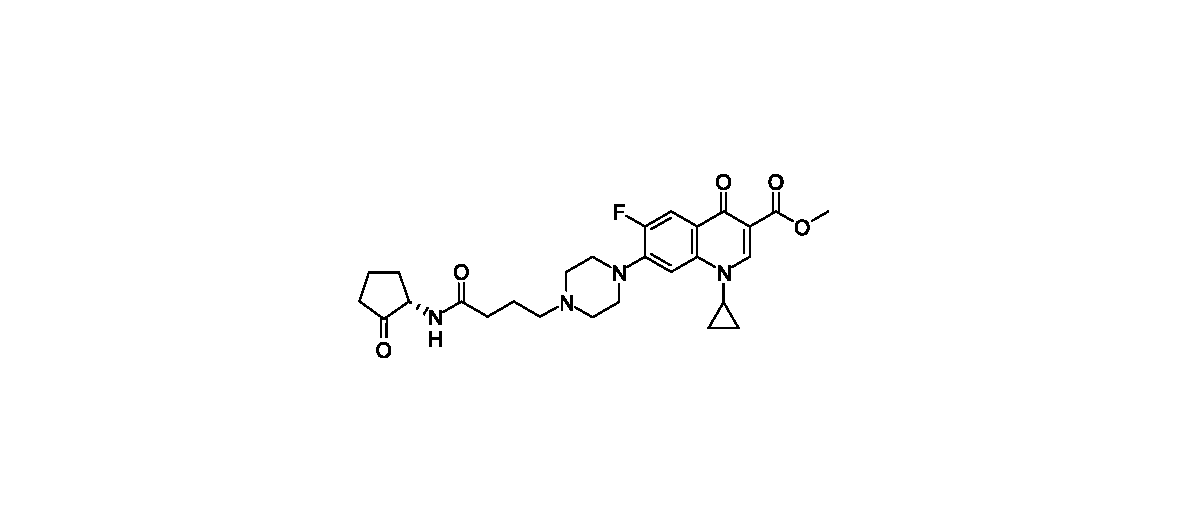
\includegraphics[scale=1]{Ocy5NH4CipMe(S).eps}
%	\end{center}
%\end{scheme}
%
%\todo{find??}
%
\subsection{Methyl (\textit{S})\hyp{}1\hyp{}cyclopropyl\hyp{}6\hyp{}fluoro\hyp{}4\hyp{}oxo\hyp{}7\hyp{}(4\hyp{}(4\hyp{}oxo\hyp{}4\hyp{}((2\hyp{}oxocyclopentyl)amin\allowbreak o)butyl)piperazin\hyp{}1\hyp{}yl)\hyp{}1,4\hyp{}dihydroquinoline\hyp{}3\hyp{}carboxylate \compound{cmpd:Ocy5NH4CipMe_S}}

%LMO-3-022

\begin{scheme}[H]
	\begin{center}
		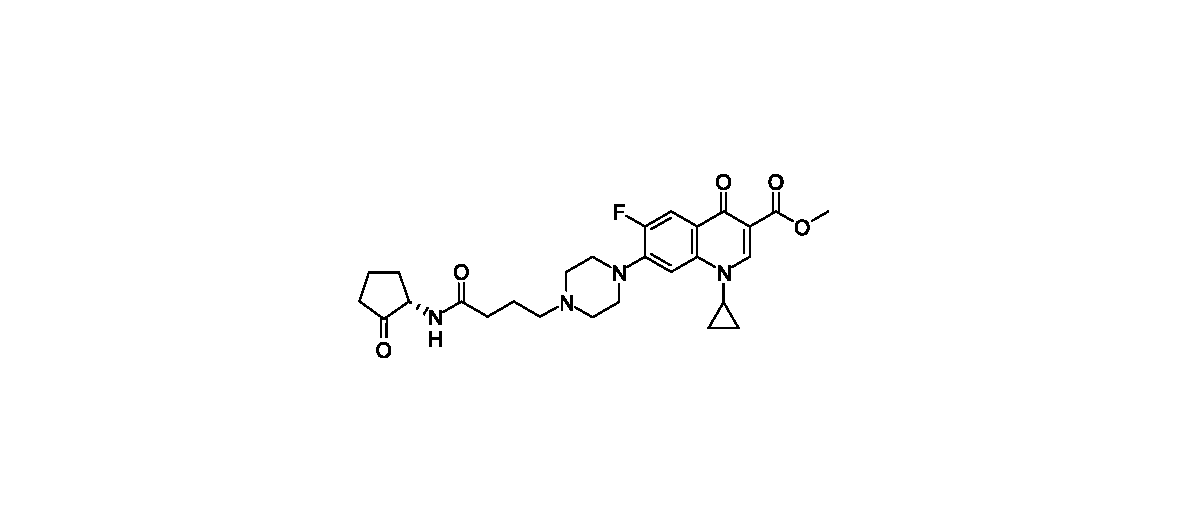
\includegraphics[scale=1]{Ocy5NH4CipMe(S).eps}
	\end{center}
\end{scheme}

Methyl 1\hyp{}cyclopropyl\hyp{}6\hyp{}fluoro\hyp{}7\hyp{}(4\hyp{}(4\hyp{}(((1\textit{S},2\textit{S})\hyp{}2\hyp{}hydroxycyclopentyl)amino)\hyp{}4\hyp{}oxobutyl)piperazin\hyp{}1\hyp{}yl)\hyp{}4\hyp{}oxo\hyp{}1,4\hyp{}dihydroquinoline\hyp{}3\hyp{}carboxylate \compound{cmpd:HOcy5NH4CipMe_SS} (20.0 mg, 38.9 $\mu$mol, 1 eq.) and Dess-Martin Periodane (32.8 mg, 77.4 $\mu$mol, 2 eq.) were stirred in \ce{CH2Cl2} (3 ml) for 6 h. The solvent was removed under reduced pressure and the residue was purified by preparatory HPLC (5-50 \% acetonitrile/water over 10 min). The combined pure fractions were evaporated under reduced pressure, then \ce{NaHCO3} (aq., sat., 30 ml) and 10 \% \textit{i}-PrOH/\ce{CHCl3} (30 ml) were added. The organic layer was removed and dried with \ce{MgSO4}, then evaporated under reduced pressure. \compound{cmpd:Ocy5NH4CipMe_S} was obtained as a white amorphous solid (11.3 mg, 22.0 $\mu$mol, 56.7 \%).
\\[1\baselineskip]
%\noindent{\textbf{TLC} \textit{R$_f$} = ?? (??)}
%\\[1\baselineskip]
%\noindent{\textbf{mp} \textit{T} / $^{\circ}$C = ?? (??)}
%\\[1\baselineskip]
%\noindent{\textbf{IR} (neat) $\nu_{max}$ / cm$^{-1}$ = ??} not enough
%\\[1\baselineskip]
\noindent{\textbf{$^{1}$H NMR} (500 MHz, DMSO d$_6$) $\delta$ / ppm = 
	8.46 (s, 1 H, \textit{ortho} to C(=O)OC\underline{H}$_3$), 
	7.78 (d, J=13.5 Hz, 1 H, \textit{ortho} to F), 
	7.45 (d, J=7.4 Hz, 1 H, \textit{meta} to F), 
	4.02 (dt, J=11.1, 8.2 Hz, 1 H, C\underline{H}NH), 
	3.73 (s, 3 H, C\underline{H}$_3$), 
	3.65 (tt, J=6.9, 3.9 Hz, 1 H, NC\underline{H}(CH$_2$)$_2$), 
	3.40 (s, 10 H, CH$_2$CH$_2$C\underline{H}$_2$N(C\underline{H}$_2$C\underline{H}$_2$)C\underline{H}$_2$C\underline{H}$_2$), 
	2.05 - 2.29 (m, 5 H, NHC(=O)C\underline{H}$_2$, C\underline{H}$_2$C(=O)CHNH and C\underline{H}HCHNH), 
	1.89 - 1.96 (m, 1 H, C\underline{H}HCH$_2$CHNH), 
	1.69 - 1.80 (m, 3 H, CH\underline{H}CH$_2$CHNH, CH\underline{H}CHNH and NHC(=O)CH$_2$C\underline{H}$_2$), 
	1.24 - 1.29 (m, 2 H, NCH(C\underline{H}H)$_2$), 
	1.07 - 1.12 (m, 2 H, NCH(CH\underline{H})$_2$)}
\\[1\baselineskip]
\noindent{\textbf{$^{13}$C NMR} (126 MHz, DMSO d$_6$) $\delta$ / ppm = 
	215.2 (\underline{C}(=O)CHNH), 
	171.7 (NH\underline{C}(=O)CH$_2$), 
	171.7 (\underline{C}(=O)CC\allowbreak (=O)\allowbreak OCH$_3$), 
	165.1 (\underline{C}(=O)OCH$_3$), 
	152.6 (d, J=246.6 Hz, \textit{ipso} to F), 
	148.4 (\underline{C}=CC(=O)OCH$_3$), 
	138.1 (\textit{para} to F), 
	109.1 (\underline{C}C(=O)OCH$_3$), 
	56.3 (\underline{C}HNH), 
	51.4 (\underline{C}H$_3$), 
	35.6 (\underline{C}H$_2$C(=O)CHNH), 
	34.8 (N\underline{C}H(CH$_2$)$_2$), 
	28.8 (\underline{C}H$_2$CHNH), 
	18.1 (\underline{C}H$_2$CH$_2$CHNH), 
	7.6 (NCH(\underline{C}H$_2$)$_2$)}
\\[1\baselineskip]
\noindent{\textbf{$^{19}$F NMR} (376.45 MHz, MeOD) $\delta$ / ppm = 
	-124.3}
\\[1\baselineskip]
\noindent{\textbf{HRMS} (ESI$^+$) \textit{m}/\textit{z} / Da = 513.2495, [M+H]$^+$ found, [\ce{C27H34FN4O5}]$^+$ requires 513.2513}
\\[1\baselineskip]
\noindent{[\bm{$\alpha$}]$_D^{20}$ / $^{\circ}$10$^{-1}$cm$^2$g$^{-1}$ = 6.7 (\textit{c} / g(100 ml)$^{-1}$ = 0.075, MeOH)}
\\[1\baselineskip]
The compound has not been reported previously.
%%\subsection{1\hyp{}cyclopropyl\hyp{}6\hyp{}fluoro\hyp{}7\hyp{}(4\hyp{}(4\hyp{}(((1\textit{S},2\textit{S})\hyp{}2\hyp{}hydroxycyclopentyl)amino)\hyp{}4\hyp{}oxobutyl)piperazin\hyp{}1\hyp{}yl)\hyp{}4\hyp{}oxo\hyp{}1,4\hyp{}dihydroquinoline\hyp{}3\hyp{}carboxylic acid \compound{cmpd:HOcy5NH4Cip(SS)}}
%%
%%%%LMO\hyp{}3\hyp{}006 (worked but not purified)
%%
%%\begin{scheme}[H]
%%	\begin{center}
%%		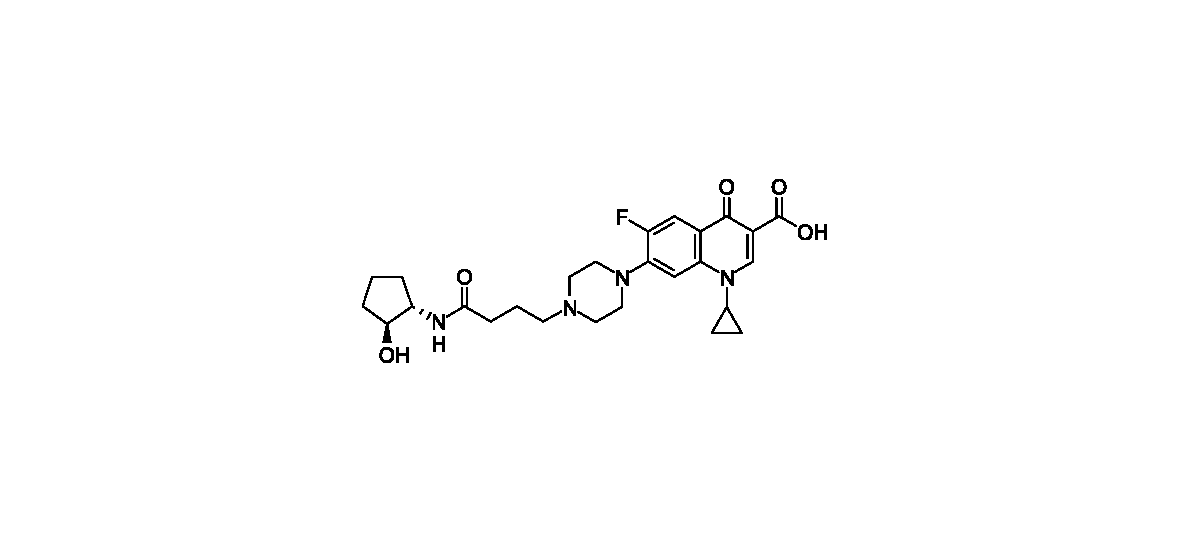
\includegraphics[scale=1]{HOcy5NH4Cip(SS).eps}
%%	\end{center}
%%\end{scheme}

\subsection{7\hyp{}(4\hyp{}(4\hyp{}(1\hyp{}(4\hyp{}(((1\textit{S},2\textit{S})\hyp{}2\hyp{}((\textit{tert}\hyp{}butyldimethylsilyl)oxy)cyclopentyl)amino)\hyp{}4\hyp{}oxobutyl)\hyp{}1\textit{H}\hyp{}1,2,3\hyp{}triazol\hyp{}4\hyp{}yl)butyl)piperazin\hyp{}1\hyp{}yl)\hyp{}1\hyp{}cyclopropyl\hyp{}6\hyp{}fluoro\hyp{}4\hyp{}oxo\hyp{}1,4\hyp{}dihydroquinoline\hyp{}3\hyp{}carboxylic acid \compound{cmpd:TBSOcy5NH4T4Cip_SS}}

%%LMO\hyp{}2\hyp{}082 (done)

\begin{scheme}[H]
	\begin{center}
		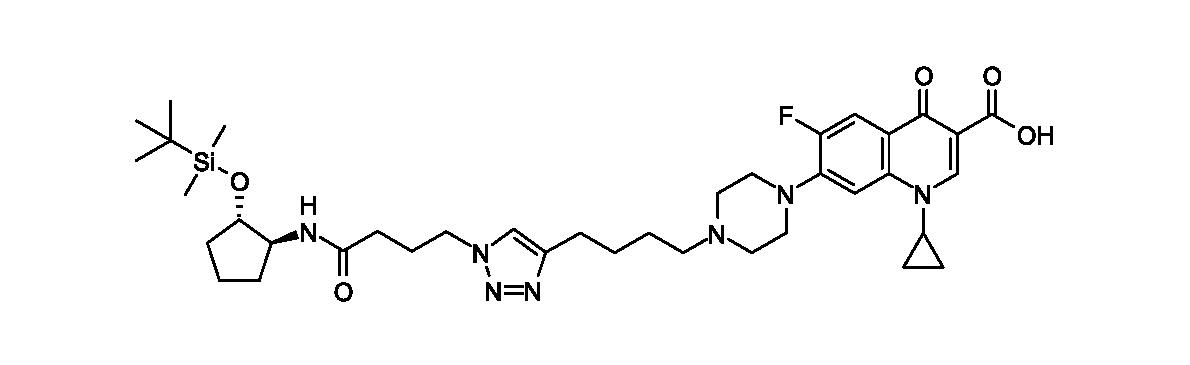
\includegraphics[scale=1]{TBSOcy5NH4T4Cip(SS).eps}
	\end{center}
\end{scheme}

1-Cyclopropyl-6-fluoro-7-(4-(hex-5-yn-1-yl)piperazin-1-yl)-4-oxo-1,4\hyp{}dihydro\-quinoline-3-carboxylic acid \compound{cmpd:Y4Cip} (42.9 mg, 104 $\mu$mol, 1 eq.) and 4\hyp{}azido\hyp{}\textit{N}\hyp{}((1\textit{S},2\textit{S})\hyp{}2\hyp{}((\textit{tert}\hyp{}butyldimethylsilyl)oxy)cyclopentyl)butanamide \compound{cmpd:TBSOcy5NH4N3_SS} (33.9 mg, 104 $\mu$mol, 1 eq.) were dissolved in 10 \% water/\textit{t}-BuOH (3 ml), and the mixture was degassed by bubbling \ce{N2} through it. 
A solution of \ce{CuSO4} and THPTA (104 $\mu$l, 10.4 $\mu$mol, 0.1 eq. 100 mM, aq.) was added, followed by a solution of sodium ascorbate (208 $\mu$l, 20.8 $\mu$mol, 0.2 eq., 100 mM, aq.). 
The mixture was stirred at room temperature under argon for 16 h, then solvent was removed under reduced pressure. The resudue was partitioned between water (10 ml) and \ce{CH2Cl2} (10 ml), the organic layer was separated and the aqueous layer was extracted again with \ce{CH2Cl2} (10 ml). The combined organic layers were dried with \ce{MgSO4} and evaporated under reduced pressure. 
\compound{cmpd:TBSOcy5NH4T4Cip_SS} was obtained as a clear glass (67.1 mg, 90.9 $\mu$mol, 87.4 \%).
\\[1\baselineskip]
%\noindent{\textbf{TLC} \textit{R$_f$} = ?? (??)}
%\\[1\baselineskip]
%\noindent{\textbf{mp} \textit{T} / $^{\circ}$C = ?? (??)}
%\\[1\baselineskip]
\noindent{\textbf{IR} (neat) $\nu_{max}$ / cm$^{-1}$ = 
	2951.3 (C-H),
	2929.2 (C-H),
	2855.5 (C-H),
	1741.0 (carboxylic acid C=O), %a bit high?
	1640.3 (amide C=O),
	1626.6 (quinolone C=O),
	1612.3 (triazole)}
\\[1\baselineskip]
\noindent{\textbf{$^{1}$H NMR} (400 MHz, \ce{CDCl3}) $\delta$ / ppm = 
	8.67 (s, 1 H, \textit{ortho} to C(=O)OH), 
	7.87 (d, \textit{J} = 13.1 Hz, 1 H, \textit{ortho} to F), 
	7.34 (s, 1 H, C\underline{H}=CCH$_2$), 
	7.33 (d, \textit{J} = 8.2 Hz, 1 H, \textit{meta} to F), 
	5.92 (t, \textit{J} = 6.6 Hz, 1 H, CHN\underline{H}), 
	4.35 (t, \textit{J} = 6.7 Hz, 2 H, C\underline{H}$_2$NCH=C), 
	3.96 - 4.02 (m, 1 H, C\underline{H}OSi), 
	3.90 - 3.96 (m, 1 H, C\underline{H}NH), 
	3.55 (tt, \textit{J} = 6.7, 4.0 Hz, 1 H, NC\underline{H}(CH$_2$)$_2$), 
	3.34 (br t, \textit{J} = 5.0 Hz, 4 H, CH$_2$N(CH$_2$C\underline{H}$_2$)CH$_2$C\underline{H}$_2$), 
	2.71 (t, \textit{J} = 7.5 Hz, 2 H, CH=CC\underline{H}$_2$), 
	2.66 (br s, 4 H, CH$_2$N(C\underline{H}$_2$)C\underline{H}$_2$), 
	2.46 (t, \textit{J} = 7.3 Hz, 2 H, C\underline{H}$_2$N(CH$_2$)CH$_2$), 
	2.03 - 2.22 (m, 5 H, C\underline{H}HCHNH, C(=O)C\underline{H}$_2$ and C(=O)CH$_2$C\underline{H}$_2$), 
	1.65 - 1.83 (m, 4 H, C\underline{H}HCHOSi, C\underline{H}HCH$_2$CHOSi and NCH=CCH$_2$C\underline{H}$_2$), 
	1.47 - 1.65 (m, 4 H, CH\underline{H}CHOSi, CH\underline{H}CH$_2$CHOSi and NCH=CCH$_2$CH$_2$C\underline{H}$_2$), 
	1.33 - 1.41 (m, 3 H, CH\underline{H}CHNH and NCH(C\underline{H}H)$_2$), 
	1.14 - 1.20 (m, 2 H, NCH(CH\underline{H})$_2$), 
	0.82 (s, 9 H, C(C\underline{H}$_3$)$_3$), 
	0.03 (s, 3 H, SiC\underline{H}$_3$), 
	0.01 (s, 3 H, SiC\underline{H}$_3$)}
\\[1\baselineskip]
\noindent{\textbf{$^{13}$C NMR} (101 MHz, \ce{CDCl3}) $\delta$ / ppm = 
	176.9 (\underline{C}(=O)CC(=O)OH), 
	170.9 (CH$_2$\underline{C}(=O)NH), 
	166.9 (\underline{C}(=O)OH), 
	153.5 (d, \textit{J} = 251.4 Hz, \textit{ipso} to F), 
	147.9 (CH=\underline{C}CH$_2$), 
	147.2 (\underline{C}=CC(=O)OH), 
	145.8 (d, \textit{J} = 10.4 Hz, \textit{ipso} to piperazine), 
	139.0 (\textit{para} to F), 
	120.9 (N\underline{C}H=CCH$_2$), 
	119.4 (d, \textit{J} = 7.8 Hz, \textit{para} to piperazine), 
	112.0 (d, \textit{J} = 23.4 Hz, \textit{ortho} to C=O and \textit{ortho} to F), 
	107.7 (\underline{C}C(=O)OH), 
	104.7 (d, \textit{J} = 3.5 Hz, \textit{meta} to C=O and \textit{meta} to F), 
	77.7 (\underline{C}HOSi), 
	58.2 (\underline{C}HNH), 
	57.9 (CH=CCH$_2$CH$_2$CH$_2$\underline{C}H$_2$N), 
	52.6 (CH=CCH$_2$CH$_2$CH$_2$CH$_2$N(\underline{C}H$_2$)\underline{C}H$_2$), 
	49.5 (d, \textit{J} = 6.1 Hz, CH=CCH$_2$CH$_2$CH$_2$CH$_2$N(CH$_2$\underline{C}H$_2$)CH$_2$\underline{C}H$_2$), 
	48.9 (d, \textit{J} = 3.5 Hz, \underline{C}H$_2$NCH=CCH$_2$), 
	35.3 (N\underline{C}H(CH$_2$)$_2$), 
	32.6 (C(=O)\underline{C}H$_2$), 
	32.6 (\underline{C}H$_2$CHOSi), 
	29.3 (\underline{C}H$_2$CHNH), 
	27.2 (CH=CCH$_2$\underline{C}H$_2$), 
	26.0 - 26.3 (C(=O)CH$_2$\underline{C}H$_2$ and CH=CCH$_2$CH$_2$\underline{C}H$_2$), 
	25.6 (C(\underline{C}H$_3$)$_3$), 
	25.4 (CH=C\underline{C}H$_2$), 
	20.4 (\underline{C}H$_2$CH$_2$CHOSi), 
	17.8 (\underline{C}(CH$_3$)$_3$), 
	8.1 (NCH(\underline{C}H$_2$)$_2$), 
	-4.8 (Si\underline{C}H$_3$)}
%\\[1\baselineskip]
%\noindent{\textbf{$^{19}$F NMR} (376.45 MHz, \ce{CDCl3}) $\delta$ / ppm = 
%	??\todo{F??}}
\\[1\baselineskip]
\noindent{\textbf{HRMS} (ESI$^+$) \textit{m}/\textit{z} / Da = 738.4164, [M+H]$^+$ found, [\ce{C38H57FN7O5Si}]$^+$ requires 738.4169}
\\[1\baselineskip]
\noindent{[\bm{$\alpha$}]$_D^{20}$ / $^{\circ}$10$^{-1}$cm$^2$g$^{-1}$ = 4.5 (\textit{c} / g(100 ml)$^{-1}$ = 0.2, MeOH)}
\\[1\baselineskip]
The compound has not been reported previously.

\subsection{1\hyp{}Cyclopropyl\hyp{}6\hyp{}fluoro\hyp{}7\hyp{}(4\hyp{}(4\hyp{}(1\hyp{}(4\hyp{}(((1\textit{R},2\textit{R})\hyp{}2\hyp{}hydroxycyclopentyl)amino)\hyp{}4\hyp{}oxobutyl)\hyp{}1\textit{H}\hyp{}1,2,3\hyp{}triazol\hyp{}4\hyp{}yl)butyl)piperazin\hyp{}1\hyp{}yl)\hyp{}4\hyp{}oxo\hyp{}1,4\hyp{}dihydroqu\allowbreak i\allowbreak n\allowbreak oline\hyp{}3\hyp{}carboxylic acid \compound{cmpd:HOcy5NH4T4Cip_RR}}

%%LMO-3-004 (done)

\begin{scheme}[H]
	\begin{center}
		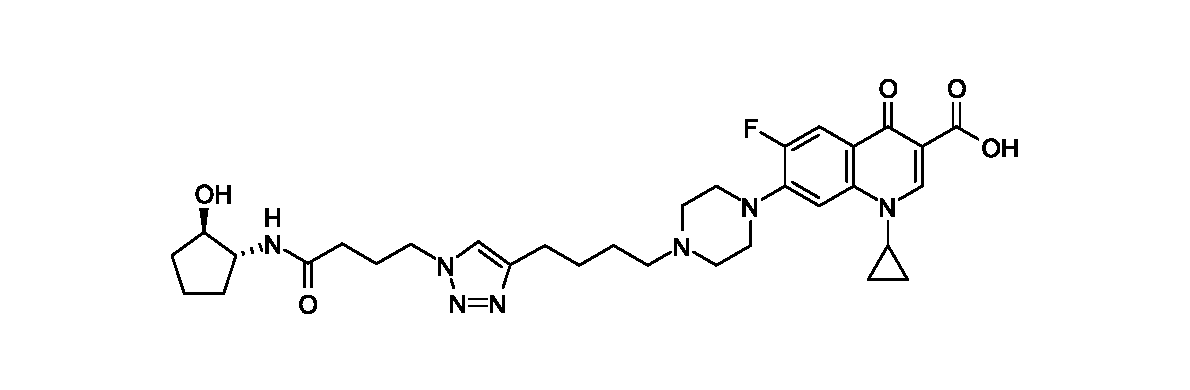
\includegraphics[scale=1]{HOcy5NH4T4Cip(RR).eps}
	\end{center}
\end{scheme}

1-Cyclopropyl-6-fluoro-7-(4-(hex-5-yn-1-yl)piperazin-1-yl)-4-oxo-1,4\hyp{}dihydro\-quinoline-3-carboxylic acid \compound{cmpd:Y4Cip} (42.9 mg, 104 $\mu$mol, 1 eq.) and 4\hyp{}azido\hyp{}\textit{N}\hyp{}((1\textit{R},2\textit{R})\hyp{}2\hyp{}hydroxycyclopentyl)butanamide \compound{cmpd:HOcy5NH4N3_RR} (22.0 mg, 104 $\mu$mol, 1 eq.) were dissolved in 10 \% water/\textit{t}-BuOH (3 ml), and the mixture was degassed by bubbling \ce{N2} through it. 
A solution of \ce{CuSO4} and THPTA (104 $\mu$l, 10.4 $\mu$mol, 0.1 eq. 100 mM, aq.) was added, followed by a solution of sodium ascorbate (208 $\mu$l, 20.8 $\mu$mol, 0.2 eq., 100 mM, aq.). 
The mixture was stirred at room temperature under argon for 16 h. Water (30 ml) and \ce{CH2Cl2} (30 ml) were added, the organic layer was separated and the aqueous layer was extracted again with \ce{CH2Cl2} (4$\times$30 ml). The combined organic layers were dried with \ce{MgSO4} and evaporated under reduced pressure. The residue was purified by preparatory HPLC (5-95 \% acetonitrile/water over 20 min). The combined pure fractions were evaporated under reduced pressure and then partitioned between \ce{NaHCO3} (aq., sat., 10 ml) and 10 \% \textit{i}-PrOH/\ce{CHCl3} (10 ml). The organic layer was dried with \ce{MgSO4} and evaporated under reduced pressure.
\compound{cmpd:HOcy5NH4T4Cip_RR} was obtained as a white amorphous solid (17.6 mg, 28.2 $\mu$mol, 27.1 \%).
\\[1\baselineskip]
%\noindent{\textbf{TLC} \textit{R$_f$} = ?? (??)}
%\\[1\baselineskip]
%\noindent{\textbf{mp} \textit{T} / $^{\circ}$C = ?? (??)}
%\\[1\baselineskip]
\noindent{\textbf{IR} (neat) $\nu_{max}$ / cm$^{-1}$ = 
	2967.0 (C-H),
	2902.2 (C-H),
	1721.4 (carboxylic acid C=O),
	1646.7 (amide C=O),
	1627.0 (quinolone C=O),
	1613.0 (triazole)}
\\[1\baselineskip]
\noindent{\textbf{$^{1}$H NMR} (700 MHz, DMSO d$_6$) $\delta$ / ppm = 
	8.64 (s, 1 H, \textit{ortho} to C(=O)OH), 
	7.87 (d, \textit{J} = 13.3 Hz, 1 H, \textit{ortho} to F), 
	7.84 (s, 1 H, C\underline{H}=CCH$_2$), 
	7.75 (d, \textit{J} = 7.1 Hz, 1 H, CHN\underline{H}), 
	7.54 (d, \textit{J} = 7.5 Hz, 1 H, \textit{meta} to F), 
	4.73 (d, \textit{J} = 3.8 Hz, 1 H, CHO\underline{H}), 
	4.29 (t, \textit{J} = 6.9 Hz, 2 H, C\underline{H}$_2$NCH=C), 
	3.78 - 3.83 (m, 1 H, NC\underline{H}(CH$_2$)$_2$), 
	3.75 - 3.78 (m, 1 H, C\underline{H}OH), 
	3.71 - 3.75 (m, 1 H, C\underline{H}NH), 
	3.31 (br t, \textit{J} = 4.3 Hz, 4 H, CH$_2$N(CH$_2$C\underline{H}$_2$)CH$_2$C\underline{H}$_2$), 
	2.63 (t, \textit{J} = 7.5 Hz, 2 H, CH=CC\underline{H}$_2$), 
	2.56 (br t, \textit{J} = 4.2 Hz, 4 H, CH$_2$N(C\underline{H}$_2$)C\underline{H}$_2$), 
	2.37 (t, \textit{J} = 7.3 Hz, 2 H, C\underline{H}$_2$N(CH$_2$)CH$_2$), 
	2.03 - 2.06 (m, 2 H, C(=O)C\underline{H}$_2$), 
	1.97 - 2.02 (m, 2 H, C(=O)CH$_2$C\underline{H}$_2$), 
	1.89 (dddd, \textit{J} = 13.1, 8.9, 7.4, 5.7 Hz, 1 H, C\underline{H}HCHNH), 
	1.75 (ddt, \textit{J} = 13.0, 8.9, 6.4, 6.4 Hz, 1 H, C\underline{H}HCHOH), 
	1.61 - 1.66 (m, 2 H, CH=CCH$_2$C\underline{H}$_2$), 
	1.57 - 1.61 (m, 1 H, C\underline{H}HCH$_2$CHOH), 
	1.54 - 1.57 (m, 1 H, CH\underline{H}CH$_2$CHOH), 
	1.49 - 1.53 (m, 2 H, CH=CCH$_2$CH$_2$C\underline{H}$_2$), 
	1.40 (ddt, \textit{J} = 13.0, 8.4, 5.3, 5.3 Hz, 1 H, CH\underline{H}CHOH), 
	1.29 - 1.32 (m, 2 H, NCH(C\underline{H}H)$_2$), 
	1.25 - 1.29 (m, 1 H, CH\underline{H}CHNH), 
	1.13 - 1.20 (m, 2 H, NCH(CH\underline{H})$_2$)}
\\[1\baselineskip]
\noindent{\textbf{$^{13}$C NMR} (175 MHz, DMSO d$_6$) $\delta$ / ppm = 
	176.3 (\underline{C}(=O)CC(=O)OH), 
	170.9 (NH\underline{C}(=O)CH$_2$), 
	166.1 (\underline{C}(=O)OH), 
	153.0 (d, \textit{J} = 251.4 Hz, \textit{ipso} to F), 
	147.9 (\underline{C}=CC(=O)OH), 
	146.9 (CH=\underline{C}CH$_2$), 
	145.2 (d, \textit{J} = 8.7 Hz, \textit{ipso} to piperazine), 
	139.2 (\textit{para} to F), 
	121.7 (N\underline{C}H=CCH$_2$), 
	118.7 (d, \textit{J} = 5.8 Hz, \textit{para} to piperazine), 
	111.0 (d, \textit{J} = 23.3 Hz, \textit{ortho} to C=O and \textit{ortho} to F), 
	106.3 (\textit{meta} to C=O and \textit{meta} to F and \underline{C}C(=O)OH), 
	76.2 (\underline{C}HOH), 
	57.6 (\underline{C}HNH), 
	57.4 (CH=CCH$_2$CH$_2$CH$_2$\underline{C}H$_2$N), 
	52.5 (CH=CCH$_2$CH$_2$CH$_2$CH$_2$N(\underline{C}H$_2$)\underline{C}H$_2$), 
	49.5 (d, \textit{J} = 4.4 Hz, CH=CCH$_2$CH$_2$CH$_2$CH$_2$N(CH$_2$\underline{C}H$_2$)CH$_2$\underline{C}H$_2$), 
	48.8 (\underline{C}H$_2$NCH=CCH$_2$), 
	35.8 (N\underline{C}H(CH$_2$)$_2$), 
	32.2 (\underline{C}H$_2$CHOH), 
	32.0 (C(=O)\underline{C}H$_2$), 
	29.5 (\underline{C}H$_2$CHNH), 
	26.9 (CH=CCH$_2$\underline{C}H$_2$), 
	26.0 (C(=O)CH$_2$\underline{C}H$_2$), 
	25.8 (CH=CCH$_2$CH$_2$\underline{C}H$_2$), 
	25.0 (CH=C\underline{C}H$_2$), 
	20.5 (\underline{C}H$_2$CH$_2$CHOH), 
	7.6 (NCH(\underline{C}H$_2$)$_2$)}
\\[1\baselineskip]
\noindent{\textbf{$^{19}$F NMR} (376.45 MHz, MeOD) $\delta$ / ppm = 
	-122.1 (s, ciprofloxacin F)}
\\[1\baselineskip]
\noindent{\textbf{HRMS} (ESI$^+$) \textit{m}/\textit{z} / Da = 624.3314, [M+H]$^+$ found, [\ce{C32H43FN7O5}]$^+$ requires 624.3310}
\\[1\baselineskip]
\noindent{[\bm{$\alpha$}]$_D^{20}$ / $^{\circ}$10$^{-1}$cm$^2$g$^{-1}$ = -3.6 (\textit{c} / g(100 ml)$^{-1}$ = 0.0833, MeOH)}
\\[1\baselineskip]
The compound has not been reported previously.

\subsection{1\hyp{}Cyclopropyl\hyp{}6\hyp{}fluoro\hyp{}7\hyp{}(4\hyp{}(4\hyp{}(1\hyp{}(4\hyp{}(((1\textit{S},2\textit{S})\hyp{}2\hyp{}hydroxycyclopentyl)amino)\hyp{}4\hyp{}oxobutyl)\hyp{}1\textit{H}\hyp{}1,2,3\hyp{}triazol\hyp{}4\hyp{}yl)butyl)piperazin\hyp{}1\hyp{}yl)\hyp{}4\hyp{}oxo\hyp{}1,4\hyp{}dihydroqu\allowbreak i\allowbreak n\allowbreak oline\hyp{}3\hyp{}carboxylic acid \compound{cmpd:HOcy5NH4T4Cip_SS}}

%%LMO\hyp{}2\hyp{}084 (reaction done but very slow, purification failed?), LMO\hyp{}2\hyp{}090 (more TBAF, quicker but small scale, lost on resin?), LMO-3-024

\begin{scheme}[H]
	\begin{center}
		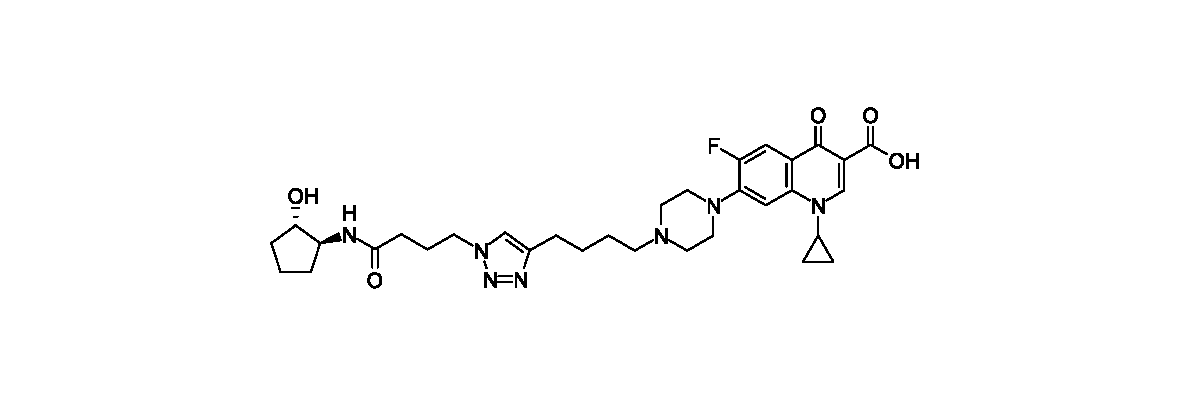
\includegraphics[scale=1]{HOcy5NH4T4Cip(SS).eps}
	\end{center}
\end{scheme}

1-Cyclopropyl-6-fluoro-7-(4-(hex-5-yn-1-yl)piperazin-1-yl)-4-oxo-1,4\hyp{}dihydro\-quinoline-3-carboxylic acid \compound{cmpd:Y4Cip} (82.0 mg, 199 $\mu$mol, 4 eq.%\todo{high?}
) and 4\hyp{}azido\hyp{}\textit{N}\hyp{}((1\textit{S},2\textit{S})\hyp{}2\hyp{}hydroxycyclopentyl)butanamide \compound{cmpd:HOcy5NH4N3_SS} (11.0 mg, 51.8 $\mu$mol, 1 eq.) were dissolved in 10 \% water/\textit{t}-BuOH (3 ml), and the mixture was degassed by bubbling \ce{N2} through it. 
A solution of \ce{CuSO4} and THPTA (156 $\mu$l, 15.6 $\mu$mol, 0.3 eq. 100 mM, aq.) was added, followed by a solution of sodium ascorbate (312 $\mu$l, 31.2 $\mu$mol, 0.6 eq., 100 mM, aq.). 
The mixture was stirred at room temperature under argon for 3 d. Water (10 ml) and 10 \% \textit{i}-PrOH/\ce{CHCl3} (10 ml) were added, then the organic layer was separated and dried with \ce{MgSO4} and evaporated under reduced pressure. 
The residue was purified by preparatory HPLC (5-95 \% acetonitrile/water over 20 min). The combined pure fractions were evaporated under reduced pressure and then partitioned between \ce{NaHCO3} (aq., sat., 10 ml) and 10 \% \textit{i}-PrOH/\ce{CHCl3} (10 ml). The organic layer was dried with \ce{MgSO4} and evaporated under reduced pressure.
\compound{cmpd:HOcy5NH4T4Cip_SS} was obtained as a white amorphous solid (7.2 mg, 11.5 $\mu$mol, 22.2 \%).
\\[1\baselineskip]
%\noindent{\textbf{TLC} \textit{R$_f$} = ?? (??)}
%\\[1\baselineskip]
%\noindent{\textbf{mp} \textit{T} / $^{\circ}$C = ?? (??)}
%\\[1\baselineskip]
\noindent{\textbf{IR} (neat) $\nu_{max}$ / cm$^{-1}$ = 
	2954.9 (C-H),
	2917.9 (C-H),
	2850.2 (C-H),
	1722.1 (carboxylic acid C=O),
	1647.3 (amide C=O),
	1626.7 (quinolone C=O)
	1611.9 (triazole)}
\\[1\baselineskip]
\noindent{\textbf{$^{1}$H NMR} (400 MHz, DMSO d$_6$) $\delta$ / ppm = 
	15.22 (br s, 1 H, C(=O)O\underline{H}), 
	8.67 (s, 1 H, \textit{ortho} to C(=O)OH), 
	7.91 (d, J=13.3 Hz, 1 H, \textit{ortho} to F), 
	7.84 (s, 1 H, C\underline{H}=CCH$_2$), 
	7.74 (d, J=6.7 Hz, 1 H, CHN\underline{H}), 
	7.56 (d, J=7.4 Hz, 1 H, \textit{meta} to F), 
	4.71 (d, J=3.7 Hz, 1 H, CHO\underline{H}), 
	4.29 (t, J=6.6 Hz, 2 H, C\underline{H}$_2$NCH=C), 
	3.82 (tt, J=6.5, 4.3 Hz, 1 H, NC\underline{H}(CH$_2$)$_2$), 
	3.69 - 3.79 (m, 2 H, C\underline{H}OH and C\underline{H}NH), 
	3.30 - 3.34 (m, 6 H, CH=CCH$_2$CH$_2$CH$_2$C\underline{H}$_2$N(C\underline{H}$_2$C\underline{H}$_2$)C\underline{H}$_2$C\underline{H}$_2$), 
	2.64 (t, J=7.4 Hz, 2 H, CH=CC\underline{H}$_2$), 
	1.95 - 2.08 (m, 4 H, C(=O)C\underline{H}$_2$C\underline{H}$_2$), 
	1.89 (dddd, J=12.8, 8.9, 7.4, 5.8 Hz, 1 H, C\underline{H}HCHNH), 
	1.75 (ddt, J=12.7, 9.0, 6.2, 6.2 Hz, 1 H, C\underline{H}HCHOH), 
	1.48 - 1.68 (m, 6 H, CH=CCH$_2$C\underline{H}$_2$C\underline{H}$_2$ and C\underline{H}$_2$CH$_2$CHOH), 
	1.40 (ddt, J=13.0, 8.3, 5.3, 5.3 Hz, 1 H, CH\underline{H}CHOH), 
	1.28 - 1.35 (m, 2 H, NCH(C\underline{H}H)$_2$), 
	1.24 - 1.31 (m, 1 H, CH\underline{H}CHNH), 
	1.15 - 1.21 (m, 2 H, NCH(CH\underline{H})$_2$)}
\\[1\baselineskip]
\noindent{\textbf{$^{13}$C NMR} (101 MHz, DMSO d$_6$) $\delta$ / ppm = 
	176.4 (\underline{C}(=O)CC(=O)OH), 
	170.9 (NH\underline{C}(=O)CH$_2$), 
	166.0 (\underline{C}(=O)OH), 
	153.0 (d, J=249.6 Hz, \textit{ipso} to F), 
	148.1 (\underline{C}=CC(=O)OH), 
	146.7 (CH=\underline{C}CH$_2$), 
	145.2 (d, J=8.3 Hz, \textit{ipso} to piperazine), 
	139.2 (\textit{para} to F), 
	121.8 (N\underline{C}H=CCH$_2$), 
	118.7 (\textit{para} to piperazine), 
	111.0 (d, J=23.2 Hz, \textit{ortho} to C=O and \textit{ortho} to F), 
	106.7 (\underline{C}C(=O)OH), 
	106.5 (\textit{meta} to C=O and \textit{meta} to F), 
	76.2 (\underline{C}HOH), 
	57.5 (\underline{C}HNH), 
	57.4 (br s, CH=CCH$_2$CH$_2$CH$_2$\underline{C}H$_2$N), 
	52.3 (br s, CH=CCH$_2$CH$_2$CH$_2$CH$_2$N(\underline{C}H$_2$)\underline{C}H$_2$), 
	49.3 (br s, CH=CCH$_2$CH$_2$CH$_2$CH$_2$N(CH$_2$\underline{C}H$_2$)CH$_2$\underline{C}H$_2$), 
	48.8 (\underline{C}H$_2$NCH=CCH$_2$), 
	35.9 (N\underline{C}H(CH$_2$)$_2$), 
	32.2 (\underline{C}H$_2$CHOH), 
	32.0 (C(=O)\underline{C}H$_2$), 
	29.4 (\underline{C}H$_2$CHNH), 
	26.7 (CH=CCH$_2$\underline{C}H$_2$), 
	26.0 (C(=O)CH$_2$\underline{C}H$_2$), 
	25.5 (CH=CCH$_2$CH$_2$\underline{C}H$_2$), 
	24.9 (CH=C\underline{C}H$_2$), 
	20.5 (\underline{C}H$_2$CH$_2$CHOH), 
	7.6 (NCH(\underline{C}H$_2$)$_2$)}
\\[1\baselineskip]
\noindent{\textbf{$^{19}$F NMR} (376.45 MHz, MeOD) $\delta$ / ppm = 
	-121.5}
\\[1\baselineskip]
\noindent{\textbf{HRMS} (ESI$^+$) \textit{m}/\textit{z} / Da = 624.3298, [M+H]$^+$ found, [\ce{C32H43FN7O5}]$^+$ requires 624.3310}
\\[1\baselineskip]
\noindent{[\bm{$\alpha$}]$_D^{20}$ / $^{\circ}$10$^{-1}$cm$^2$g$^{-1}$ = -25.0 (\textit{c} / g(100 ml)$^{-1}$ = 0.08, MeOH)%\todo{explain discrepancy}}
\\[1\baselineskip]
The compound has not been reported previously.

%\subsection{(\textit{S})\hyp{}1\hyp{}cyclopropyl\hyp{}6\hyp{}fluoro\hyp{}4\hyp{}oxo\hyp{}7\hyp{}(4\hyp{}(4\hyp{}(1\hyp{}(4\hyp{}oxo\hyp{}4\hyp{}((2\hyp{}oxocyclopentyl)amino)\hyp{}butyl)\hyp{}1H\hyp{}1,2,3\hyp{}triazol\hyp{}4\hyp{}yl)butyl)piperazin\hyp{}1\hyp{}yl)\hyp{}1,4\hyp{}dihydroquinoline\hyp{}3\hyp{}carboxylic acid \compound{cmpd:Ocy5NH4T4Cip(S)}}
%
%\begin{scheme}[H]
%	\begin{center}
%		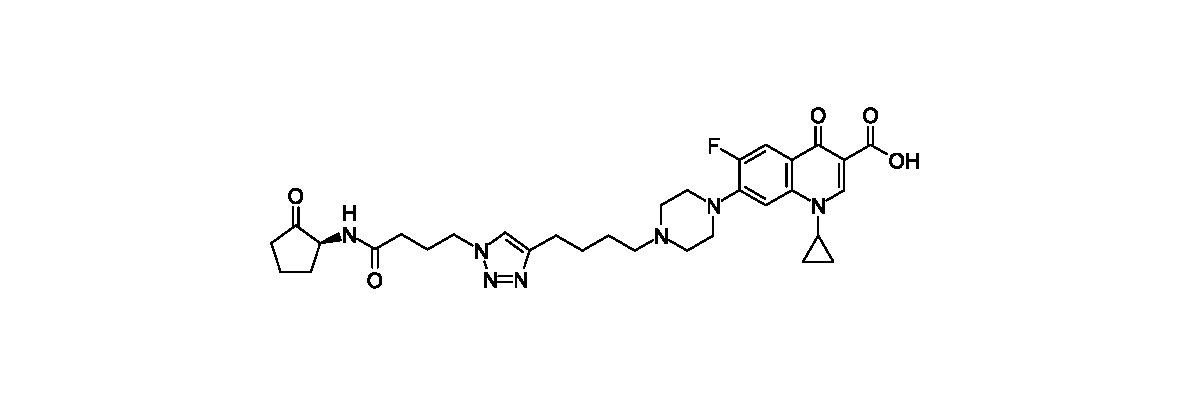
\includegraphics[scale=1]{Ocy5NH4T4Cip(S).eps}
%	\end{center}
%\end{scheme}
%
%\subsection{(\textit{R})\hyp{}1\hyp{}cyclopropyl\hyp{}6\hyp{}fluoro\hyp{}4\hyp{}oxo\hyp{}7\hyp{}(4\hyp{}(4\hyp{}(1\hyp{}(4\hyp{}oxo\hyp{}4\hyp{}((2\hyp{}oxocyclopentyl)amino)\hyp{}butyl)\hyp{}1H\hyp{}1,2,3\hyp{}triazol\hyp{}4\hyp{}yl)butyl)piperazin\hyp{}1\hyp{}yl)\hyp{}1,4\hyp{}dihydroquinoline\hyp{}3\hyp{}carboxylic acid \compound{cmpd:Ocy5NH4T4Cip(R)}}
%
%\begin{scheme}[H]
%	\begin{center}
%		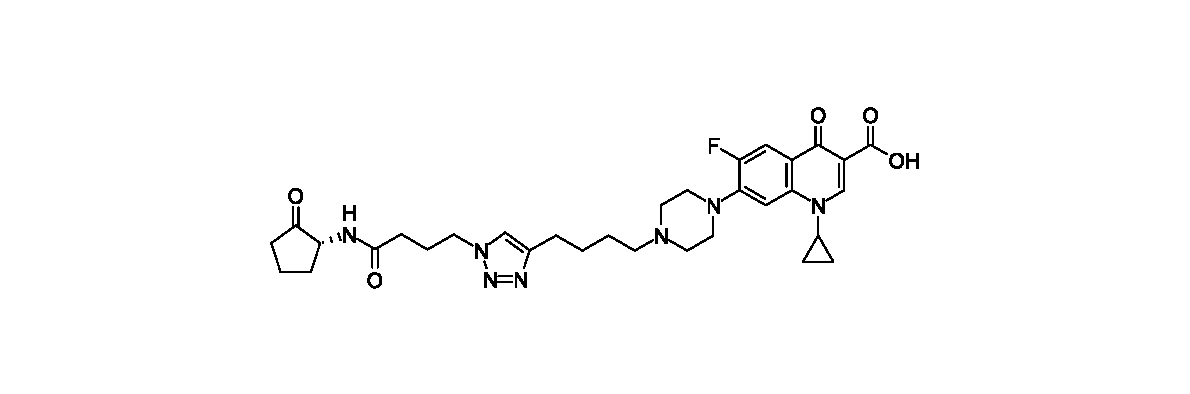
\includegraphics[scale=1]{Ocy5NH4T4Cip(R).eps}
%	\end{center}
%\end{scheme}



\subsection{(\textit{trans})\hyp{}2\hyp{}Aminocyclohexan\hyp{}1\hyp{}ol \compound{cmpd:HOcy6NH2}}

%%LMO\hyp{}3\hyp{}007, LMO\hyp{}3\hyp{}008, LMO\hyp{}3\hyp{}009, LMO\hyp{}3\hyp{}011 (main, done)

\begin{scheme}[H]
	\begin{center}
		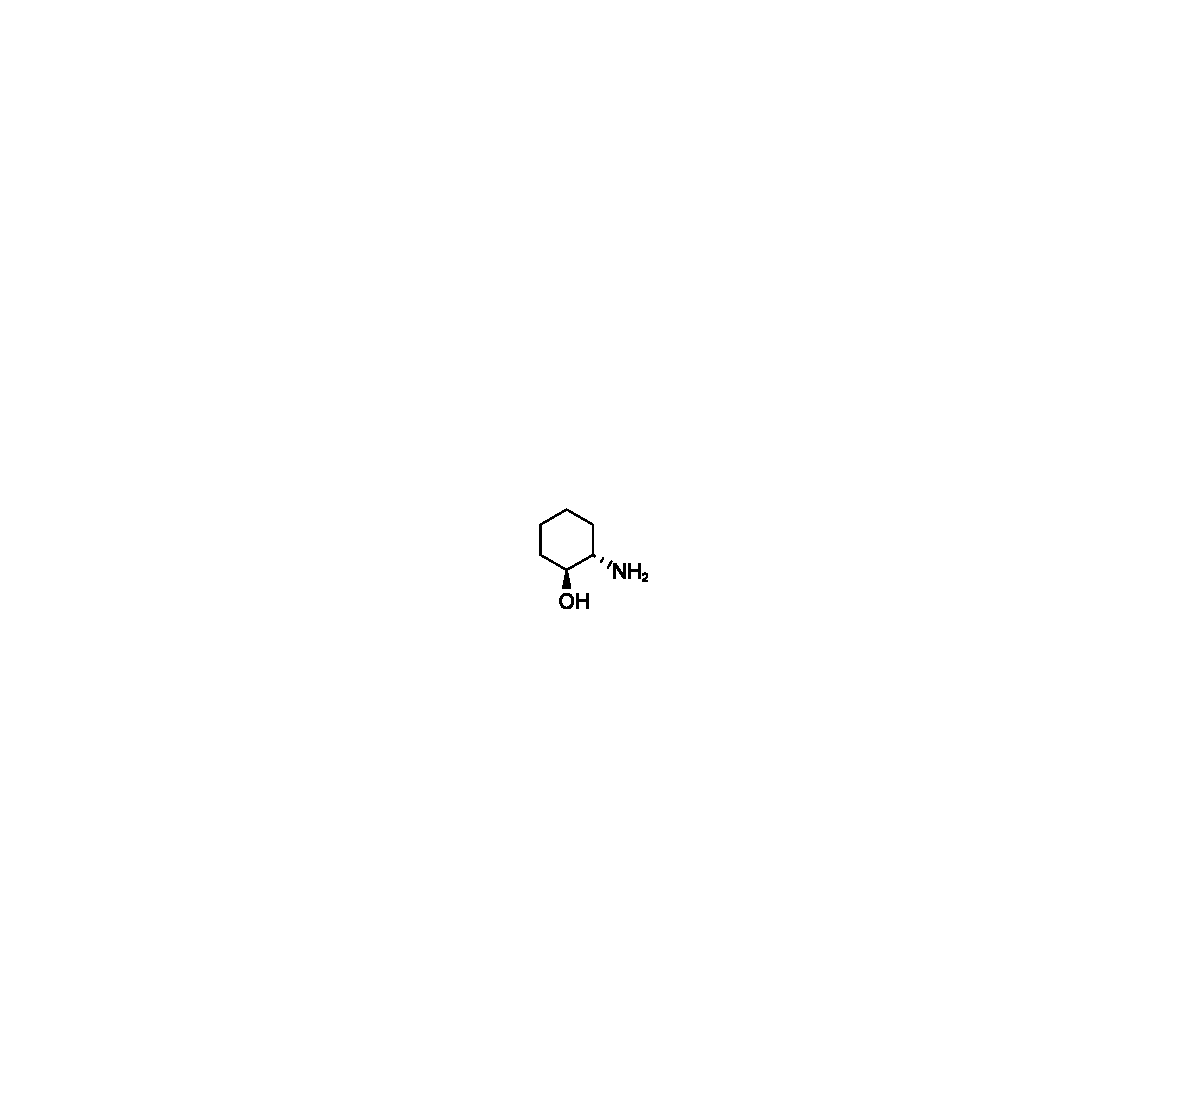
\includegraphics[scale=1]{HOcy6NH2.eps}
	\end{center}
\end{scheme}

Cyclohexene oxide \compound{cmpd:cy6ox} (10 ml, 9.70 g, 98.8 mmol, 1 eq.), \ce{NH3} (90 ml, 35 \% w/w aq., 27.7 g, 791 mmol, 8 eq.) and MeOH (100 ml) were stirred at r.t. for 72 h. The solvent was removed by blowing a stream of \ce{N2} over it, followed by evaporation under high vacuum.%\todo{phrasing?}.
\compound{cmpd:HOcy6NH2} was obtained as a white amorphous solid (9.90 g, 85.2 mmol, 86.2 \%)
\\[1\baselineskip]
\noindent{\textbf{TLC} \textit{R$_f$} = 0.04 (30 \% MeOH/\ce{CH2Cl2})}
\\[1\baselineskip]
\noindent{\textbf{IR} (neat) $\nu_{max}$ / cm$^{-1}$ = 
	3350.4 (N-H),
	3306.2 (br, O-H),
	2926.9 (C-H),
	2852.6 (C-H)}
\\[1\baselineskip]
\noindent{\textbf{$^{1}$H NMR} (400 MHz, \ce{CDCl3}) $\delta$ / ppm = 
	3.01 (td, \textit{J} = 9.4, 4.8 Hz, 1 H, C\underline{H}OH), 
	2.80 - 2.92 (m, 2 H, O\underline{H} and N\underline{H}$_2$), 
	2.35 (ddd, \textit{J} = 11.1, 9.1, 4.1 Hz, 1 H, C\underline{H}NH$_2$), 
	1.77 - 1.84 (m, 1 H, C\underline{H}HCHOH), 
	1.69 - 1.76 (m, 1 H, C\underline{H}HCHNH$_2$), 
	1.56 - 1.66 (m, 1 H, C\underline{H}HCH$_2$CHOH), 
	1.45 - 1.56 (m, 1 H, C\underline{H}HCH$_2$CHNH$_2$), 
	1.07 - 1.19 (m, 3 H, CH\underline{H}CH$_2$CHOH, CH\underline{H}CH$_2$CHNH$_2$ and CH\underline{H}CHOH), 
	0.94 - 1.05 (m, 1 H, CH\underline{H}CHNH$_2$)}
\\[1\baselineskip]
\noindent{\textbf{$^{13}$C NMR} (101 MHz, \ce{CDCl3}) $\delta$ / ppm = 
	75.4 (\underline{C}HOH), 
	56.6 (\underline{C}HN$_2$), 
	33.8 (\underline{C}H$_2$CHOH and \underline{C}H$_2$CHN$_2$), 
	24.7 (\underline{C}H$_2$CH$_2$CHN$_2$), 
	24.6 (\underline{C}H$_2$CH$_2$CHOH)}
\\[1\baselineskip]
\noindent{\textbf{HRMS} (ESI$^+$) \textit{m}/\textit{z} / Da = 116.1070, [M+H]$^+$ found, [\ce{C6H14NO}]$^+$ requires 116.1070}
\\[1\baselineskip]
The data are consistent with the literature\cite{Xue2006}.
	
\subsection{4\hyp{}Chloro\hyp{}\textit{N}\hyp{}((\textit{trans})\hyp{}2\hyp{}hydroxycyclohexyl)butanamide  \compound{cmpd:HOcy6NH4Cl}}

%%LMO\hyp{}3\hyp{}010 (ugh at purification), LMO\hyp{}3\hyp{}014 (done)

\begin{scheme}[H]
	\begin{center}
		\includegraphics[scale=1]{HOcy6NH4Cl.eps}
	\end{center}
\end{scheme}

(\textit{trans})\hyp{}2\hyp{}Aminocyclohexan\hyp{}1\hyp{}ol \compound{cmpd:HOcy6NH2} (1.04 g, 9.03 mmol, 1 eq.), TEA (1.65 ml, 1.20 g, 11.8 mmol, 1.3 eq.) and \ce{CH2Cl2} (50 ml) were stirred at 0 $^\circ$C. 4-Chlorobutyryl chloride \compound{cmpd:Cl4Cl} (1.22 ml, 1.54 g, 10.9 mmol, 1.2 eq.) was added dropwise over 5 min. The mixture was stirred at 0 $^\circ$C for 30 min, then water (50 ml) was added. The organic layer was separated off, and the aqueous layer was extracted with 10 \% \textit{i}-PrOH/\ce{CHCl3} (2$\times$50 ml). The combined organic layers were dried with \ce{MgSO4}, concentrated under reduced pressure and purified by column chromatography (\ce{SiO2}, 0-100 \% EtOAc/\ce{Et2O}). The combined organic fractions were dried with \ce{MgSO4} and evaporated under reduced pressure. \compound{cmpd:HOcy6NH4Cl} was obtained as white needles (1.51 g, 6.87 mmol, 76.1 \%).
\\[1\baselineskip]
\noindent{\textbf{TLC} \textit{R$_f$} = 0.19 (\ce{Et2O})}
\\[1\baselineskip]
\noindent{\textbf{mp} \textit{T} / $^{\circ}$C = 72.5-75.7 (\textit{i}-PrOH, \ce{CHCl3})}
\\[1\baselineskip]
\noindent{\textbf{IR} (neat) $\nu_{max}$ / cm$^{-1}$ = 
	3289.9 (N-H),
	3250.0 (O-H),
	2927.6 (C-H),
	2857.1 (C-H),
	1629.2 (amide C=O)}
\\[1\baselineskip]
\noindent{\textbf{$^{1}$H NMR} (400 MHz, MeOD) $\delta$ / ppm = 
	3.60 (t, \textit{J} = 6.6 Hz, 2 H, C\underline{H}$_2$Cl), 
	3.51 - 3.60 (m, 1 H, C\underline{H}NH), 
	3.28 - 3.39 (m, 1 H, C\underline{H}OH), 
	2.37 (td, \textit{J} = 7.4, 2.3 Hz, 2 H, C(=O)C\underline{H}$_2$), 
	2.06 (quin, \textit{J} = 7.0 Hz, 2 H, C(=O)CH$_2$C\underline{H}$_2$), 
	1.97 - 2.01 (m, 1 H, C\underline{H}HCHOH), 
	1.85 - 1.93 (m, 1 H, C\underline{H}HCHNH), 
	1.70 - 1.77 (m, 1 H, C\underline{H}HCH$_2$CHOH), 
	1.64 - 1.70 (m, 1 H, C\underline{H}HCH$_2$CHNH), 
	1.24 - 1.35 (m, 3 H, CH\underline{H}CH$_2$CHOH, CH\underline{H}CH$_2$CHNH and CH\underline{H}CHOH), 
	1.13 - 1.25 (m, 1 H, CH\underline{H}CHNH$_2$)}
\\[1\baselineskip]
\noindent{\textbf{$^{13}$C NMR} (101 MHz, MeOD) $\delta$ / ppm = 
	175.0 (\underline{C}(=O)), 
	74.1 (\underline{C}HOH), 
	56.3 (\underline{C}HNH), 
	45.3 (\underline{C}H$_2$Cl), 
	35.6 (\underline{C}H$_2$CHOH), 
	34.5 (C(=O)\underline{C}H$_2$), 
	32.7 (\underline{C}H$_2$CHNH), 
	30.1 (C(=O)CH$_2$\underline{C}H$_2$), 
	25.8 (\underline{C}H$_2$CH$_2$CHNH), 
	25.5 (\underline{C}H$_2$CH$_2$CHOH)}
\\[1\baselineskip]
\noindent{\textbf{HRMS} (ESI$^+$) \textit{m}/\textit{z} / Da = 242.0925, [M+Na]$^+$ found, [\ce{C10H18ClNNaO2}]$^+$ requires 242.0924}
\\[1\baselineskip]
The compound has not been reported previously.

\subsection{4\hyp{}Azido\hyp{}\textit{N}\hyp{}((\textit{trans})\hyp{}2\hyp{}hydroxycyclohexyl)butanamide  \compound{cmpd:HOcy6NH4N3}}

%%LMO\hyp{}3\hyp{}012 (small, didn't purify), LMO\hyp{}3\hyp{}015 (done)

\begin{scheme}[H]
	\begin{center}
		\includegraphics[scale=1]{HOcy6NH4N3.eps}
	\end{center}
\end{scheme}

4\hyp{}Chloro\hyp{}\textit{N}\hyp{}((\textit{trans})\hyp{}2\hyp{}hydroxycyclohexyl)butanamide  \compound{cmpd:HOcy6NH4Cl} (345 mg, 1.57 mmol, 1 eq.) and \ce{NaN3} (180 mg, 2.77 mmol, 1.75 eq.) were stirred in DMF (12 ml) at 50 $^\circ$C for 16 h. Water (50 ml) and 10 \% \textit{i}-PrOH/\ce{CHCl3} (50 ml) were added, and the organic layer was removed. The aqueous layer was extracted again with 10 \% \textit{i}-PrOH/\ce{CHCl3} (50 ml) and the combined organic fractions were dried with \ce{MgSO4}. The solvent was evaporated under reduced pressure, and then by using a \ce{N2} stream. \compound{cmpd:HOcy6NH4N3} was obtained as large white prisms (347 mg, 1.53 mmol, 97.5 \%).
\\[1\baselineskip]
\noindent{\textbf{TLC} \textit{R$_f$} = 0.23 (EtOAc)}
\\[1\baselineskip]
\noindent{\textbf{mp} \textit{T} / $^{\circ}$C = 74.5-75.7 (\textit{i}-PrOH, \ce{CHCl3})}
\\[1\baselineskip]
\noindent{\textbf{IR} (neat) $\nu_{max}$ / cm$^{-1}$ =
	3299.0 (N-H),
	3207.8 (O-H),
	2944.3 (C-H),
	2927.9 (C-H),
	2859.2 (C-H),
	2089.2 (azide),
	1624.0 (amide C=O)}
\\[1\baselineskip]
\noindent{\textbf{$^{1}$H NMR} (400 MHz, MeOD) $\delta$ / ppm = 
	7.87 (d, \textit{J} = 7.9 Hz, 1 H, N\underline{H}), 
	5.27 (d, \textit{J} = 4.3 Hz, 1 H, O\underline{H}), 
	3.56 (td, \textit{J} = 10.5, 4.4 Hz, 1 H, C\underline{H}NH), 
	3.28 - 3.41 (m, 3 H, C\underline{H}OH and C\underline{H}$_2$N$_3$), 
	2.30 (td, \textit{J} = 7.4, 2.7 Hz, 2 H, C(=O)C\underline{H}$_2$), 
	1.95 - 2.03 (m, 1 H, C\underline{H}HCHOH), 
	1.87 (m, 3 H, C(=O)CH$_2$C\underline{H}$_2$ and C\underline{H}HCHNH), 
	1.70 - 1.76 (m, 1 H, C\underline{H}HCH$_2$CHOH), 
	1.63 - 1.70 (m, 1 H, C\underline{H}HCH$_2$CHNH), 
	1.25 - 1.38 (m, 3 H, CH\underline{H}CH$_2$CHOH, CH\underline{H}CH$_2$CHNH and CH\underline{H}CHOH), 
	1.14 - 1.24 (m, 1 H, CH\underline{H}CHNH$_2$)}
\\[1\baselineskip]
\noindent{\textbf{$^{13}$C NMR} (101 MHz, MeOD) $\delta$ / ppm = 
	175.1 (\underline{C}(=O)), 
	74.0 (\underline{C}HOH), 
	56.3 (\underline{C}HNH), 
	52.0 (\underline{C}H$_2$N$_3$), 
	35.5 (\underline{C}H$_2$CHOH), 
	34.3 (C(=O)\underline{C}H$_2$), 
	32.7 (\underline{C}H$_2$CHNH), 
	26.3 (C(=O)CH$_2$\underline{C}H$_2$), 
	25.8 (\underline{C}H$_2$CH$_2$CHNH), 
	25.5 (\underline{C}H$_2$CH$_2$CHOH)}
\\[1\baselineskip]
\noindent{\textbf{HRMS} (ESI$^+$) \textit{m}/\textit{z} / Da = 249.1331, [M+Na]$^+$ found, [\ce{C10H18N4NaO2}]$^+$ requires 249.1327}
\\[1\baselineskip]
The compound has not been reported previously.

\subsection{Methyl 1\hyp{}cyclopropyl\hyp{}6\hyp{}fluoro\hyp{}7\hyp{}(4\hyp{}(4\hyp{}(((\textit{trans})\hyp{}2\hyp{}hydroxycyclohexyl)amino)\hyp{}4\hyp{}oxobutyl)piperazin\hyp{}1\hyp{}yl)\hyp{}4\hyp{}oxo\hyp{}1,4\hyp{}dihydroquinoline\hyp{}3\hyp{}carboxylate \compound{cmpd:HOcy6NH4CipMe}}

%%LMO\hyp{}3\hyp{}013 (done)

\begin{scheme}[H]
	\begin{center}
		\includegraphics[scale=1]{HOcy6NH4CipMe.eps}
	\end{center}
\end{scheme}

4\hyp{}(4\hyp{}(1\hyp{}Cyclopropyl\hyp{}6\hyp{}fluoro\hyp{}3\hyp{}(methoxycarbonyl)\hyp{}4\hyp{}oxo\hyp{}1,4\hyp{}dihydroquinolin\hyp{}7\hyp{}yl)piperazin\hyp{}1\hyp{}yl)butanoic\hfill acid trifluoroacetate \compound{cmpd:HOO4CipMeTFA} (200 mg, 0.367 mmol, 1 eq.), (\textit{trans})\hyp{}2\hyp{}aminocyclohexan\hyp{}1\hyp{}ol \compound{cmpd:HOcy6NH2} (91.1 mg, 0.791 mmol, 2.1 eq.), 1-ethyl-3-(3-dimethylaminopropyl)carbodi\allowbreak imide hydrochloride (112 mg, 0.584 mmol, 1.6 eq.), 1-hydroxyben\allowbreak zotriazole (96 mg, 0.710 mmol, 1.9 eq.) and DIPEA (192 $\mu$l, 142 mg, 1.10 mmol, 3 eq.) were dissolved in DMF (5 ml) and stirred at r.t. for 16 h. The solvent was removed using a stream of \ce{N2} and the residue was purified by preparatory HPLC (5-50 \% acetonitrile/water over 10 min). The combined pure fractions were evaporated under reduced pressure and then partitioned between \ce{NaHCO3} (aq., sat., 10 ml) and \ce{CH2Cl2} (10 ml). The organic layer was dried with \ce{MgSO4} and evaporated under reduced pressure. \compound{cmpd:HOcy6NH4CipMe} was obtained as a white amorphous solid (73.0 mg, 0.142 mmol, 38.7 \%).
\\[1\baselineskip]
%\noindent{\textbf{TLC} \textit{R$_f$} = ?? (??)}
%\\[1\baselineskip]
%\noindent{\textbf{mp} \textit{T} / $^{\circ}$C = ?? (??)}
%\\[1\baselineskip]
\noindent{\textbf{IR} (neat) $\nu_{max}$ / cm$^{-1}$ = 
	3302.5 (N-H),
	2929.8 (C-H),
	2850.6 (C-H),
	2832.9 (C-H),
	1698.1 (ester C=O),
	1646.4 (amide C=O),
	1613.8 (quinolone C=O)}
\\[1\baselineskip]
\noindent{\textbf{$^{1}$H NMR} (400 MHz, MeOD) $\delta$ / ppm = 
	8.60 (s, 1 H, \textit{ortho} to C(=O)OC\underline{H}$_3$), 
	7.79 (d, \textit{J} = 13.5 Hz, 1 H, \textit{ortho} to F), 
	7.46 (d, \textit{J} = 7.2 Hz, 1 H, \textit{meta} to F), 
	3.84 (s, 3 H, C\underline{H}$_3$), 
	3.62 - 3.68 (m, 1 H, NC\underline{H}(CH$_2$)$_2$), 
	3.58 (td, \textit{J} = 10.3, 4.2 Hz, 1 H, C\underline{H}NH), 
	3.38 (br s, 4 H, CH$_2$N(CH$_2$C\underline{H}$_2$)CH$_2$C\underline{H}$_2$), 
	3.32 - 3.36 (m, 1 H, C\underline{H}OH), 
	2.83 (br s, 4 H, CH$_2$N(C\underline{H}$_2$)C\underline{H}$_2$), 
	2.60 (t, \textit{J} = 7.3 Hz, 2 H, C(=O)CH$_2$CH$_2$C\underline{H}$_2$N), 
	2.32 (td, \textit{J} = 7.1, 3.1 Hz, 2 H, C(=O)C\underline{H}$_2$), 
	1.96 - 2.04 (m, 1 H, C\underline{H}HCHOH), 
	1.87 - 1.96 (m, 3 H, C\underline{H}HCHNH and C(=O)CH$_2$C\underline{H}$_2$), 
	1.72 - 1.77 (m, 1 H, C\underline{H}HCH$_2$CHOH), 
	1.66 - 1.72 (m, 1 H, C\underline{H}HCH$_2$CHNH), 
	1.25 - 1.39 (m, 5 H, CH\underline{H}CHOH, CH\underline{H}CH$_2$CHOH, CH\underline{H}CH$_2$CHNH and NCH(C\underline{H}H)$_2$), 
	1.15 - 1.25 (m, 3 H, CH\underline{H}CHOH and NCH(CH\underline{H})$_2$)}
\\[1\baselineskip]
\noindent{\textbf{$^{13}$C NMR} (101 MHz, MeOD) $\delta$ / ppm = 
	175.8 (CH$_2$\underline{C}(=O)NH), 
	175.3 (\underline{C}(=O)CC(=O)OCH$_3$), 
	166.8 (\underline{C}(=O)\allowbreak OCH$_3$), 
	154.9 (d, \textit{J} = 248.8 Hz, \textit{ipso} to F), 
	150.2 (\underline{C}=CC(=O)OCH$_3$), 
	146.1 (d, \textit{J} = 10.8 Hz, \textit{ipso} to piperazine), 
	139.9 (\textit{para} to F), 
	123.5 (d, \textit{J} = 7.5 Hz, \textit{para} to piperazine), 
	113.2 (d, \textit{J} = 23.2 Hz, \textit{ortho} to C=O and \textit{ortho} to F), 
	110.2 (\underline{C}C(=O)OCH$_3$), 
	107.2 (\textit{meta} to C=O and \textit{meta} to F), 
	74.1 (\underline{C}HOH), 
	58.9 (C(=O)CH$_2$CH$_2$\underline{C}H$_2$N), 
	56.4 (\underline{C}HNH), 
	54.0 (C(=O)CH$_2$CH$_2$CH$_2$N(\underline{C}H$_2$)\underline{C}H$_2$), 
	52.3 (\underline{C}H$_3$), 
	50.5 (d, \textit{J} = 5.0 Hz, C(=O)CH$_2$CH$_2$CH$_2$N(CH$_2$\underline{C}H$_2$)CH$_2$\underline{C}H$_2$), 
	36.4 (N\underline{C}H(CH$_2$)$_2$), 
	35.7 (\underline{C}H$_2$CHOH), 
	35.1 (C(=O)\underline{C}H$_2$), 
	32.8 (\underline{C}H$_2$CHNH), 
	25.9 (\underline{C}H$_2$CH$_2$CHNH), 
	25.5 (\underline{C}H$_2$CH$_2$CHOH), 
	23.5 (C(=O)CH$_2$\underline{C}H$_2$), 
	8.7 (NCH(\underline{C}H$_2$)$_2$)}
\\[1\baselineskip]
\noindent{\textbf{$^{19}$F NMR} (376.45 MHz, MeOD) $\delta$ / ppm = 
	-124.7 (ciprofloxacin F)}
\\[1\baselineskip]
\noindent{\textbf{HRMS} (ESI$^+$) \textit{m}/\textit{z} / Da = 529.2827, [M+H]$^+$ found, [C28H38FN4O5]$^+$ requires 529.2826}
\\[1\baselineskip]
The compound has not been reported previously.

\subsection{Methyl 1\hyp{}cyclopropyl\hyp{}6\hyp{}fluoro\hyp{}4\hyp{}oxo\hyp{}7\hyp{}(4\hyp{}(4\hyp{}oxo\hyp{}4\hyp{}((2\hyp{}oxocyclohexyl)amino)\hyp{}butyl)piperazin\hyp{}1\hyp{}yl)\hyp{}1,4\hyp{}dihydroquinoline\hyp{}3\hyp{}carboxylate \compound{cmpd:Ocy6NH4CipMe}}

%%LMO\hyp{}3\hyp{}017 (done)

\begin{scheme}[H]
	\begin{center}
		\includegraphics[scale=1]{Ocy6NH4CipMe.eps}
	\end{center}
\end{scheme}

Methyl 1\hyp{}cyclopropyl\hyp{}6\hyp{}fluoro\hyp{}7\hyp{}(4\hyp{}(4\hyp{}(((\textit{trans})\hyp{}2\hyp{}hydroxycyclohexyl)amino)\hyp{}4\hyp{}oxobutyl)piperazin\hyp{}1\hyp{}yl)\hyp{}4\hyp{}oxo\hyp{}1,\allowbreak 4\hyp{}dihydroquinoline\hyp{}3\hyp{}carboxylate \compound{cmpd:HOcy6NH4CipMe} (5.2 mg, 9.84 $\mu$mol, 1 eq.) and Dess-Martin periodane (16.4 mg, 38.7 $\mu$mol, 4 eq.) were stirred in \ce{CH2Cl2} (3 ml) for 6 h. The solvent was removed under reduced pressure and the residue was purified by preparatory HPLC (5-95 \% acetonitrile/water over 20 min). The combined pure fractions were evaporated under reduced pressure to a volume of 20 ml, then \ce{NaHCO3} (aq., sat., 30 ml) and 10 \% \textit{i}-PrOH/\ce{CHCl3} (30 ml) were added. The organic layer was dried with \ce{MgSO4} and evaporated under reduced pressure. \compound{cmpd:Ocy6NH4CipMe} was obtained as a white amorphous solid (3.6 mg, 6.8 $\mu$mol, 69.1 \%).
\\[1\baselineskip]
\noindent{\textbf{TLC} \textit{R$_f$} = 0.74 (30 \% MeOH/\ce{CH2Cl2})}
\\[1\baselineskip]
%\noindent{\textbf{mp} \textit{T} / $^{\circ}$C = ?? (??)}
%\\[1\baselineskip]
\noindent{\textbf{IR} (neat) $\nu_{max}$ / cm$^{-1}$ = 
	2921.2 (C-H),
	2851.6 (C-H),
	1721.4 (ketone C=O),
	1698.0 (ester C=O),
	1639.3 (amide C=O),
	1620.0 (quinolone C=O)}
\\[1\baselineskip]
\noindent{\textbf{$^{1}$H NMR} (400 MHz, DMSO d$_6$) $\delta$ / ppm = 
	8.45 (s, 1 H, \textit{ortho} to C(=O)OC\underline{H}$_3$), 
	7.87 (d, \textit{J} = 6.2 Hz, 1 H, N\underline{H}), 
	7.76 (d, \textit{J} = 13.4 Hz, 1 H, \textit{ortho} to F), 
	7.44 (d, \textit{J} = 7.5 Hz, 1 H, \textit{meta} to F), 
	4.42 (dddd, \textit{J} = 13.0, 7.6, 6.0, 1.0 Hz, 1 H, C\underline{H}NH), 
	3.73 (s, 3 H, C\underline{H}$_3$), 
	3.65 (tt, \textit{J} = 7.1, 3.9 Hz, 1 H, NC\underline{H}(CH$_2$)$_2$), 
	3.25 (br s, 4 H, CH$_2$N(CH$_2$C\underline{H}$_2$)CH$_2$C\underline{H}$_2$), 
	2.58 (br s, 4 H, CH$_2$N(C\underline{H}$_2$)C\underline{H}$_2$), 
	2.45 - 2.53 (m, 1 H, C\underline{H}HC(=O)CHNH), 
	2.36 (br s, 2 H, C(=O)CH$_2$CH$_2$C\underline{H}$_2$N), 
	2.26 (dtt, \textit{J} = 13.4, 2.6, 2.6, 1.6, 1.6 Hz, 1 H, CH\underline{H}C(=O)CHNH), 
	2.16 - 2.22 (m, 2 H, C(=O)C\underline{H}$_2$CH$_2$CH$_2$N), 
	2.12 (ddq, \textit{J} = 12.7, 6.0, 2.8, 2.8, 2.8 Hz, 1 H, C\underline{H}HCHNH), 
	2.00 (ddquin, \textit{J} = 13.2, 6.0, 2.9, 2.9, 2.9, 2.9 Hz, 1 H, C\underline{H}HCH$_2$C(=O)), 
	1.65 - 1.83 (m, 4 H, C\underline{H}$_2$CH$_2$CHNH), 
	1.41 - 1.56 (m, 2 H, CH\underline{H}CHNH and CH\underline{H}CH$_2$C(=O)), 
	1.20 - 1.30 (m, 2 H, NCH(C\underline{H}H)$_2$), 
	1.05 - 1.13 (m, 2 H, NCH(CH\underline{H})$_2$)}
\\[1\baselineskip]
\noindent{\textbf{$^{13}$C NMR} (101 MHz, DMSO d$_6$) $\delta$ / ppm = 
	207.5 (\underline{C}(=O)CHNH), 
	171.7 (\underline{C}(=O)CC(=O)OCH$_3$), 
	171.6 (CH$_2$\underline{C}(=O)NH), 
	165.0 (\underline{C}(=O)OCH$_3$), 
	152.6 (d, \textit{J} = 247.6 Hz, \textit{ipso} to F), 
	148.3 (\underline{C}=CC(=O)OCH$_3$), 
	143.9 (br s, \textit{ipso} to piperazine), 
	138.1 (\textit{para} to F), 
	121.8 (d, \textit{J} = 6.4 Hz, \textit{para} to piperazine), 
	111.5 (d, \textit{J} = 22.4 Hz, \textit{ortho} to C=O and \textit{ortho} to F), 
	109.0 (\underline{C}C(=O)OCH$_3$), 
	106.3 (\textit{meta} to C=O and \textit{meta} to F), 
	57.0 (\underline{C}HNH and C(=O)CH$_2$CH$_2$\underline{C}H$_2$N), 
	52.3 (br s, C(=O)CH$_2$CH$_2$CH$_2$N(\underline{C}H$_2$)\underline{C}H$_2$), 
	51.3 (\underline{C}H$_3$), 
	49.5 (br s, C(=O)CH$_2$CH$_2$CH$_2$N(CH$_2$\underline{C}H$_2$)CH$_2$\underline{C}H$_2$), 
	40.6 (C\underline{H}$_2$C(=O)CHNH), 
	34.8 (N\underline{C}H(CH$_2$)$_2$), 
	33.9 (C\underline{H}$_2$CHNH), 
	32.9 (C(=O)\underline{C}H$_2$CH$_2$CH$_2$N), 
	27.2 (C\underline{H}$_2$CH$_2$C(=O)CHNH), 
	23.8 (C\underline{H}$_2$CH$_2$CHNH), 
	22.4 (br s, C(=O)CH$_2$\underline{C}H$_2$\allowbreak CH$_2$N), 
	7.6 (NCH(\underline{C}H$_2$)$_2$)}
\\[1\baselineskip]
\noindent{\textbf{$^{19}$F NMR} (376.45 MHz, DMSO d$_6$) $\delta$ / ppm = 
	-124.3 (ciprofloxacin F)}
\\[1\baselineskip]
\noindent{\textbf{HRMS} (ESI$^+$) \textit{m}/\textit{z} / Da = 527.2654, [M+H]$^+$ found, [\ce{C28H36FN4O5}]$^+$ requires 527.2670}
\\[1\baselineskip]
The compound has not been reported previously.
	
\subsection{1\hyp{}Cyclopropyl\hyp{}6\hyp{}fluoro\hyp{}7\hyp{}(4\hyp{}(4\hyp{}(1\hyp{}(4\hyp{}(((\textit{trans})\hyp{}2\hyp{}hydroxycyclohexyl)amino)\hyp{}4\hyp{}oxobutyl)\hyp{}1\textit{H}\hyp{}1,2,3\hyp{}triazol\hyp{}4\hyp{}yl)butyl)piperazin\hyp{}1\hyp{}yl)\hyp{}4\hyp{}oxo\hyp{}1,4\hyp{}dihydroquinoline\hyp{}3\hyp{}carboxylic acid \compound{cmpd:HOcy6NH4T4Cip}}

%%LMO\hyp{}3\hyp{}016 (done)

\begin{scheme}[H]
	\begin{center}
		\includegraphics[scale=1]{HOcy6NH4T4Cip.eps}
	\end{center}
\end{scheme}

1-Cyclopropyl-6-fluoro-7-(4-(hex-5-yn-1-yl)piperazin-1-yl)-4-oxo-1,4\hyp{}dihydro\-quinoline-3-carboxylic acid \compound{cmpd:Y4Cip} (40 mg, 97.2 $\mu$mol, 1 eq.) and 4\hyp{}azido\hyp{}\textit{N}\hyp{}((\textit{trans})\hyp{}2\hyp{}hydroxycyclohexyl)butanamide  \compound{cmpd:HOcy6NH4N3} (22.0 mg, 97.2 $\mu$mol, 1 eq.) were dissolved in 10 \% water/\textit{t}-BuOH (3 ml), and the mixture was degassed by bubbling \ce{N2} through it. 
A solution of \ce{CuSO4} and THPTA (97.2 $\mu$l, 9.72 $\mu$mol, 0.1 eq. 100 mM, aq.) was added, followed by a solution of sodium ascorbate (194 $\mu$l, 19.4 $\mu$mol, 0.2 eq., 100 mM, aq.). 
The mixture was stirred at r.t. under argon for 16 h. Water (50 ml) and 10 \% \textit{i}-PrOH/\ce{CHCl3} (50 ml) were added, then the organic layer was separated, dried with \ce{MgSO4} and evaporated under reduced pressure. The residue was purified by preparatory HPLC (5-70 \% acetonitrile/water over 15 min). 
The combined pure fractions were evaporated under reduced pressure and then partitioned between \ce{NaHCO3} (aq., sat., 50 ml) and 10 \% \textit{i}-PrOH/\ce{CHCl3} (50 ml). The organic layer was dried with \ce{MgSO4} and evaporated under reduced pressure.
\compound{cmpd:HOcy6NH4T4Cip} was obtained as a white amorphous solid (30.3 mg, 47.5 $\mu$mol, 48.9 \%).
\\[1\baselineskip]
%\noindent{\textbf{TLC} \textit{R$_f$} = ?? (??)}
%\\[1\baselineskip]
%\noindent{\textbf{mp} \textit{T} / $^{\circ}$C = ?? (??)}
%\\[1\baselineskip]
\noindent{\textbf{IR} (neat) $\nu_{max}$ / cm$^{-1}$ = 
	3345.4 (N-H),
	2927.6 (C-H),
	2859.6 (C-H),
	2814.7 (C-H),
	1727.0 (carboxylic acid C=O),
	1641.7 (amide C=O),
	1625.8 (quinolone C=O),
	1619.0 (triazole)}
\\[1\baselineskip]
\noindent{\textbf{$^{1}$H NMR} (400 MHz, DMSO d$_6$) $\delta$ / ppm = 
	8.64 (s, 1 H, \textit{ortho} to C(=O)OH), 
	7.86 (d, \textit{J} = 13.9 Hz, 1 H, \textit{ortho} to F), 
	7.84 (s, 1 H, C\underline{H}=CCH$_2$), 
	7.64 (d, \textit{J} = 8.1 Hz, 1 H, N\underline{H}), 
	7.54 (d, \textit{J} = 7.5 Hz, 1 H, \textit{meta} to F), 
	4.54 (d, \textit{J} = 4.7 Hz, 1 H, O\underline{H}), 
	4.30 (t, \textit{J} = 6.8 Hz, 2 H, C(=O)CH$_2$CH$_2$C\underline{H}$_2$N), 
	3.77 - 3.86 (m, 1 H, NC\underline{H}(CH$_2$)$_2$), 
	3.33 - 3.40 (m, 1 H, C\underline{H}NH), 
	3.31 (br t, \textit{J} = 4.8, 4.8 Hz, 4 H, CH=CCH$_2$CH$_2$CH$_2$N(CH$_2$C\underline{H}$_2$)CH$_2$C\underline{H}$_2$), 
	3.14 - 3.24 (m, 1 H, C\underline{H}OH), 
	2.63 (t, \textit{J} = 7.4 Hz, 2 H, CH=CC\underline{H}$_2$), 
	2.56 (br t, \textit{J} = 4.6, 4.6 Hz, 4 H, CH=CCH$_2$CH$_2$CH$_2$N(C\underline{H}$_2$)C\underline{H}$_2$), 
	2.38 (t, \textit{J} = 6.9 Hz, 2 H, CH=CCH$_2$CH$_2$CH$_2$C\underline{H}$_2$N), 
	2.04 - 2.08 (m, 2 H, C(=O)C\underline{H}$_2$CH$_2$CH$_2$N), 
	1.96 - 2.04 (m, 2 H, C(=O)CH$_2$C\underline{H}$_2$CH$_2$N), 
	1.78 - 1.87 (m, 1 H, C\underline{H}HCHOH), 
	1.69 - 1.78 (m, 1 H, C\underline{H}HCHNH), 
	1.63 (quin, \textit{J} = 7.5 Hz, 2 H, CH=CCH$_2$C\underline{H}$_2$CH$_2$CH$_2$N), 
	1.54 - 1.60 (m, 1 H, C\underline{H}HCH$_2$OH), 
	1.51 (quin, \textit{J} = 7.4 Hz, 2 H, CH=CCH$_2$CH$_2$C\underline{H}$_2$CH$_2$N), 
	1.28 - 1.35 (m, 1 H, NCH(C\underline{H}H)$_2$), 
	1.11 - 1.22 (m, 5 H, NCH(CH\underline{H})$_2$, CH\underline{H}CHOH, CH\underline{H}CH$_2$CHOH and C\underline{H}$_2$CH$_2$CHNH), 
	1.04 - 1.13 (m, 1 H, CH\underline{H}CHNH)}
\\[1\baselineskip]
\noindent{\textbf{$^{13}$C NMR} (101 MHz, DMSO d$_6$) $\delta$ / ppm = 
	176.4 (\underline{C}(=O)CC(=O)OH), 
	170.9 (CH$_2$\underline{C}(=O)NH), 
	166.0 (\underline{C}(=O)OH), 
	153.1 (d, \textit{J} = 252.1 Hz, \textit{ipso} to F), 
	148.0 (\underline{C}=CC(=O)OH), 
	146.9 (CH=\underline{C}CH$_2$), 
	145.3 (d, \textit{J} = 10.0 Hz, \textit{ipso} to piperazine), 
	139.2 (\textit{para} to F), 
	121.8 (N\underline{C}H=CCH$_2$), 
	118.5 (d, \textit{J} = 8.3 Hz, \textit{para} to piperazine), 
	110.9 (d, \textit{J} = 23.2 Hz, \textit{ortho} to C=O and \textit{ortho} to F), 
	106.7 (\underline{C}C(=O)OH), 
	106.3 (d, \textit{J} = 3.3 Hz, \textit{meta} to C=O and \textit{meta} to F), 
	71.4 (\underline{C}HOH), 
	57.4 (CH=CCH$_2$CH$_2$CH$_2$\underline{C}H$_2$N), 
	54.2 (\underline{C}HNH), 
	52.4 (CH=CCH$_2$CH$_2$CH$_2$CH$_2$N(\underline{C}H$_2$)\underline{C}H$_2$), 
	49.5 (CH=CCH$_2$CH$_2$CH$_2$CH$_2$N(CH$_2$\underline{C}H$_2$)CH$_2$CH$_2$), 
	49.5 (CH=CCH$_2$CH$_2$CH$_2$CH$_2$N(CH$_2$CH$_2$)CH$_2$\underline{C}H$_2$), 
	48.8 (C(=O)CH$_2$CH$_2$\underline{C}H$_2$NCH=C), 
	35.9 (N\underline{C}H(CH$_2$)$_2$), 
	34.1 (C\underline{H}$_2$CHOH), 
	32.3 (C(=O)\underline{C}H$_2$CH$_2$CH$_2$NCH=C), 
	31.1 (C\underline{H}$_2$CHNH), 
	26.9 (CH=CCH$_2$\underline{C}H$_2$CH$_2$CH$_2$N), 
	26.1 (C(=O)CH$_2$\underline{C}H$_2$CH$_2$NCH=C), 
	25.8 (CH=CCH$_2$CH$_2$\underline{C}H$_2$\allowbreak CH$_2$N), 
	25.0 (CH=C\underline{C}H$_2$CH$_2$CH$_2$CH$_2$N), 
	24.2 (C\underline{H}$_2$CH$_2$CHNH), 
	23.8 (C\underline{H}$_2$CH$_2$CHOH), 
	7.6 (NCH(\underline{C}H$_2$)$_2$)}
\\[1\baselineskip]
\noindent{\textbf{$^{19}$F NMR} (376.45 MHz, DMSO d$_6$) $\delta$ / ppm = 
	-121.4 (ciprofloxacin F)}
\\[1\baselineskip]
\noindent{\textbf{HRMS} (ESI$^+$) \textit{m}/\textit{z} / Da = 638.3480, [M+H]$^+$ found, [\ce{C33H45FN7O5}]$^+$ requires 638.3466}
\\[1\baselineskip]
The compound has not been reported previously.

\subsection{1\hyp{}Cyclopropyl\hyp{}6\hyp{}fluoro\hyp{}4\hyp{}oxo\hyp{}7\hyp{}(4\hyp{}(4\hyp{}(1\hyp{}(4\hyp{}oxo\hyp{}4\hyp{}((2\hyp{}oxocyclohexyl)amino)bu\allowbreak t\allowbreak yl)\hyp{}1\textit{H}\hyp{}1,2,3\hyp{}triazol\hyp{}4\hyp{}yl)butyl)piperazin\hyp{}1\hyp{}yl)\hyp{}1,4\hyp{}dihydroquinoline\hyp{}3\hyp{}carb\allowbreak o\allowbreak x\allowbreak ylic acid \compound{cmpd:Ocy6NH4T4Cip}}

%%LMO\hyp{}3\hyp{}018 (done? awaiting NMR)

\begin{scheme}[H]
	\begin{center}
		\includegraphics[scale=1]{Ocy6NH4T4Cip.eps}
	\end{center}
\end{scheme}

1\hyp{}Cyclopropyl\hyp{}6\hyp{}fluoro\hyp{}7\hyp{}(4\hyp{}(4\hyp{}(1\hyp{}(4\hyp{}(((\textit{trans})\hyp{}2\hyp{}hydroxycyclohexyl)amino)\hyp{}4\hyp{}oxobutyl)\hyp{}1H\hyp{}1,2,3\hyp{}triazol\hyp{}4\hyp{}yl)but\allowbreak yl)piperazin\hyp{}1\hyp{}yl)\hyp{}4\hyp{}oxo\hyp{}1,4\hyp{}dihydroquinoline\hyp{}3\hyp{}carboxylic acid \compound{cmpd:HOcy6NH4T4Cip} (15.0 mg, 23.6 mmol, 1 eq.) and Dess-Martin periodane (35.0 mg, 82.5 mmol, 3.5 eq.) were stirred in \ce{CH2Cl2} (3 ml) for 4 h. The solvent was removed under reduced pressure and the residue was purified by preparatory HPLC (5-70 \% acetonitrile/water over 15 min). The combined pure fractions were evaporated under reduced pressure, then \ce{NaHCO3} (aq., sat., 30 ml) and 10 \% \textit{i}-PrOH/\ce{CHCl3} (30 ml) were added. The organic layer was dried with \ce{MgSO4} and evaporated under reduced pressure. \compound{cmpd:Ocy6NH4T4Cip} was obtained as a clear gum (11.7 mg, 18.4 $\mu$mol, 78.0 \%).
%\\[1\baselineskip]
%\noindent{\textbf{TLC} \textit{R$_f$} = ?? (??)}
%\\[1\baselineskip]
%\noindent{\textbf{mp} \textit{T} / $^{\circ}$C = ?? (??)}
\\[1\baselineskip]
\noindent{\textbf{IR} (neat) $\nu_{max}$ / cm$^{-1}$ = 
	2941.2 (C-H),
	2859.8 (C-H),
	1719.8 (carboxylic acid C=O and ketone C=O),
	1656.8 (amide C=O),
	1625.6 (quinolone C=O),
	1613.5 (triazole)}
\\[1\baselineskip]
\noindent{\textbf{$^{1}$H NMR} (500 MHz, DMSO d$_6$) $\delta$ / ppm = 
	8.65 (s, 1 H, \textit{ortho} to C(=O)OH), 
	7.94 (d, J=7.7 Hz, 1 H, N\underline{H}), 
	7.88 (d, J=13.4 Hz, 1 H, \textit{ortho} to F), 
	7.85 (s, 1 H, C\underline{H}=CCH$_2$), 
	7.55 (d, J=7.3 Hz, 1 H, \textit{meta} to F), 
	4.40 (dddd, J=12.8, 7.6, 6.1, 1.1 Hz, 1 H), 
	4.31 (t, J=7.0 Hz, 1 H, C(=O)CH$_2$CH$_2$C\underline{H}HN), 
	4.31 (t, J=6.9 Hz, 1 H, C(=O)CH$_2$CH$_2$CH\underline{H}$_2$N), 
	3.74 - 3.84 (m, 1 H, NC\underline{H}(CH$_2$)$_2$), 
	3.31 (br. s, 4 H, CH$_2$CH$_2$CH$_2$N(CH$_2$C\underline{H}$_2$)CH$_2$C\underline{H}$_2$), 
	2.64 (t, J=7.5 Hz, 2 H, CH=CC\underline{H}$_2$), 
	2.56 (br t, J=5.0, 5.0 Hz, 4 H, CH$_2$CH$_2$CH$_2$N(C\underline{H}$_2$)C\underline{H}$_2$), 
	2.45 - 2.52 (m, 1 H, C\underline{H}HC(=O)), 
	2.38 (t, J=7.1 Hz, 2 H, CH=CCH$_2$CH$_2$CH$_2$C\underline{H}$_2$N), 
	2.25 (dtt, J=13.4, 2.6, 2.6, 1.6, 1.6 Hz, 1 H, CH\underline{H}C(=O)), 
	2.07 - 2.17 (m, 3 H, C(=O)C\underline{H}$_2$CH$_2$CH$_2$N and C\underline{H}HCHNH), 
	1.96 - 2.05 (m, 3 H, C(=O)CH$_2$C\underline{H}$_2$CH$_2$N and C\underline{H}HCH$_2$C(=O)), 
	1.68 - 1.81 (m, 2 H, C\underline{H}HCH$_2$CHNH), 
	1.64 (quin, J=7.5 Hz, 2 H, CH=CCH$_2$C\underline{H}$_2$CH$_2$CH$_2$N), 
	1.40 - 1.56 (m, 5 H, CH\underline{H}CH$_2$C(=O), CH\underline{H}CHNH and CH=CCH$_2$CH$_2$C\underline{H}$_2$CH$_2$N), 
	1.27 - 1.34 (m, 2 H, NCH(C\underline{H}H)$_2$), 
	1.13 - 1.20 (m, 2 H, NCH(CH\underline{H})$_2$)}
\\[1\baselineskip]
\noindent{\textbf{$^{13}$C NMR} (126 MHz, DMSO d$_6$) $\delta$ / ppm = 
	207.4 (\underline{C}(=O)CHNH), 
	176.3 (\underline{C}(=O)CC(=O)OH), 
	170.8 (CH$_2$\underline{C}\allowbreak (=O)\allowbreak NH), 
	166.0 (\underline{C}(=O)OH), 
	153.0 (d, J=246.4 Hz, \textit{ipso} to F), 
	147.9 (\underline{C}=CC(=O)OH), 
	146.8 (CH=\underline{C}CH$_2$), 
	145.1 (d, J=10.1 Hz, \textit{ipso} to piperazine), 
	139.1 (\textit{para} to F), 
	121.7 (N\underline{C}H=CCH$_2$), 
	118.7 (d, J=6.9 Hz, \textit{para} to piperazine), 
	110.9 (d, J=23.0 Hz, \textit{ortho} to C=O and \textit{ortho} to F), 
	106.3 (\underline{C}C(=O)OH, and \textit{meta} to C=O and \textit{meta} to F), 
	57.3 (CH=CCH$_2$CH$_2$CH$_2$\underline{C}H$_2$N), 
	57.0 (\underline{C}HNH), 
	52.4 (CH$_2$CH$_2$CH$_2$N(\underline{C}H$_2$)\underline{C}H$_2$), 
	49.5 (CH$_2$CH$_2$CH$_2$N\allowbreak (CH$_2$\underline{C}H$_2$)CH$_2$CH$_2$), 
	49.5 (CH$_2$CH$_2$CH$_2$N(CH$_2$CH$_2$)CH$_2$\underline{C}H$_2$), 
	48.7 (C(=O)CH$_2$CH$_2$\underline{C}H$_2$NCH=C), 
	40.5 (\underline{C}H$_2$C\allowbreak (=O)), 
	35.8 (N\underline{C}H(CH$_2$)$_2$), 
	33.7 (\underline{C}H$_2$CHNH), 
	31.8 (C(=O)\underline{C}H$_2$CH$_2$CH$_2$NCH=C), 
	27.1 (\underline{C}H$_2$CH$_2$C(=O)), 
	26.9 (CH=CCH$_2$\underline{C}H$_2$CH$_2$CH$_2$N), 
	26.0 (C(=O)CH$_2$\underline{C}H$_2$CH$_2$NCH=C), 
	25.7 (CH=CCH$_2$CH$_2$\underline{C}H$_2$CH$_2$N), 
	24.9 (CH=C\underline{C}H$_2$CH$_2$CH$_2$CH$_2$N), 
	23.8 (\underline{C}H$_2$CH$_2$CHNH), 
	7.6 (NCH(\underline{C}H$_2$)$_2$)}
\\[1\baselineskip]
\noindent{\textbf{$^{19}$F NMR} (376 MHz, DMSO d$_6$) $\delta$ / ppm = 
	-121.7 (s, ciprofloxacin F)%}\todo{some TFA}}
\\[1\baselineskip]
\noindent{\textbf{HRMS} (ESI$^+$) \textit{m}/\textit{z} / Da = 636.3303, [M+H]$^+$ found, [\ce{C33H43FN7O5}]$^+$ requires 636.3310}
\\[1\baselineskip]
The compound has not been reported previously.